% Options for packages loaded elsewhere
\PassOptionsToPackage{unicode}{hyperref}
\PassOptionsToPackage{hyphens}{url}
\PassOptionsToPackage{dvipsnames,svgnames,x11names}{xcolor}
%
\documentclass[
  letterpaper,
  DIV=11,
  numbers=noendperiod]{scrreprt}

\usepackage{amsmath,amssymb}
\usepackage{iftex}
\ifPDFTeX
  \usepackage[T1]{fontenc}
  \usepackage[utf8]{inputenc}
  \usepackage{textcomp} % provide euro and other symbols
\else % if luatex or xetex
  \usepackage{unicode-math}
  \defaultfontfeatures{Scale=MatchLowercase}
  \defaultfontfeatures[\rmfamily]{Ligatures=TeX,Scale=1}
\fi
\usepackage{lmodern}
\ifPDFTeX\else  
    % xetex/luatex font selection
\fi
% Use upquote if available, for straight quotes in verbatim environments
\IfFileExists{upquote.sty}{\usepackage{upquote}}{}
\IfFileExists{microtype.sty}{% use microtype if available
  \usepackage[]{microtype}
  \UseMicrotypeSet[protrusion]{basicmath} % disable protrusion for tt fonts
}{}
\makeatletter
\@ifundefined{KOMAClassName}{% if non-KOMA class
  \IfFileExists{parskip.sty}{%
    \usepackage{parskip}
  }{% else
    \setlength{\parindent}{0pt}
    \setlength{\parskip}{6pt plus 2pt minus 1pt}}
}{% if KOMA class
  \KOMAoptions{parskip=half}}
\makeatother
\usepackage{xcolor}
\setlength{\emergencystretch}{3em} % prevent overfull lines
\setcounter{secnumdepth}{5}
% Make \paragraph and \subparagraph free-standing
\makeatletter
\ifx\paragraph\undefined\else
  \let\oldparagraph\paragraph
  \renewcommand{\paragraph}{
    \@ifstar
      \xxxParagraphStar
      \xxxParagraphNoStar
  }
  \newcommand{\xxxParagraphStar}[1]{\oldparagraph*{#1}\mbox{}}
  \newcommand{\xxxParagraphNoStar}[1]{\oldparagraph{#1}\mbox{}}
\fi
\ifx\subparagraph\undefined\else
  \let\oldsubparagraph\subparagraph
  \renewcommand{\subparagraph}{
    \@ifstar
      \xxxSubParagraphStar
      \xxxSubParagraphNoStar
  }
  \newcommand{\xxxSubParagraphStar}[1]{\oldsubparagraph*{#1}\mbox{}}
  \newcommand{\xxxSubParagraphNoStar}[1]{\oldsubparagraph{#1}\mbox{}}
\fi
\makeatother


\providecommand{\tightlist}{%
  \setlength{\itemsep}{0pt}\setlength{\parskip}{0pt}}\usepackage{longtable,booktabs,array}
\usepackage{calc} % for calculating minipage widths
% Correct order of tables after \paragraph or \subparagraph
\usepackage{etoolbox}
\makeatletter
\patchcmd\longtable{\par}{\if@noskipsec\mbox{}\fi\par}{}{}
\makeatother
% Allow footnotes in longtable head/foot
\IfFileExists{footnotehyper.sty}{\usepackage{footnotehyper}}{\usepackage{footnote}}
\makesavenoteenv{longtable}
\usepackage{graphicx}
\makeatletter
\def\maxwidth{\ifdim\Gin@nat@width>\linewidth\linewidth\else\Gin@nat@width\fi}
\def\maxheight{\ifdim\Gin@nat@height>\textheight\textheight\else\Gin@nat@height\fi}
\makeatother
% Scale images if necessary, so that they will not overflow the page
% margins by default, and it is still possible to overwrite the defaults
% using explicit options in \includegraphics[width, height, ...]{}
\setkeys{Gin}{width=\maxwidth,height=\maxheight,keepaspectratio}
% Set default figure placement to htbp
\makeatletter
\def\fps@figure{htbp}
\makeatother
% definitions for citeproc citations
\NewDocumentCommand\citeproctext{}{}
\NewDocumentCommand\citeproc{mm}{%
  \begingroup\def\citeproctext{#2}\cite{#1}\endgroup}
\makeatletter
 % allow citations to break across lines
 \let\@cite@ofmt\@firstofone
 % avoid brackets around text for \cite:
 \def\@biblabel#1{}
 \def\@cite#1#2{{#1\if@tempswa , #2\fi}}
\makeatother
\newlength{\cslhangindent}
\setlength{\cslhangindent}{1.5em}
\newlength{\csllabelwidth}
\setlength{\csllabelwidth}{3em}
\newenvironment{CSLReferences}[2] % #1 hanging-indent, #2 entry-spacing
 {\begin{list}{}{%
  \setlength{\itemindent}{0pt}
  \setlength{\leftmargin}{0pt}
  \setlength{\parsep}{0pt}
  % turn on hanging indent if param 1 is 1
  \ifodd #1
   \setlength{\leftmargin}{\cslhangindent}
   \setlength{\itemindent}{-1\cslhangindent}
  \fi
  % set entry spacing
  \setlength{\itemsep}{#2\baselineskip}}}
 {\end{list}}
\usepackage{calc}
\newcommand{\CSLBlock}[1]{\hfill\break\parbox[t]{\linewidth}{\strut\ignorespaces#1\strut}}
\newcommand{\CSLLeftMargin}[1]{\parbox[t]{\csllabelwidth}{\strut#1\strut}}
\newcommand{\CSLRightInline}[1]{\parbox[t]{\linewidth - \csllabelwidth}{\strut#1\strut}}
\newcommand{\CSLIndent}[1]{\hspace{\cslhangindent}#1}

\usepackage{fontspec}
\usepackage{multirow}
\usepackage{multicol}
\usepackage{colortbl}
\usepackage{hhline}
\newlength\Oldarrayrulewidth
\newlength\Oldtabcolsep
\usepackage{longtable}
\usepackage{array}
\usepackage{hyperref}
\usepackage{float}
\usepackage{wrapfig}
\KOMAoption{captions}{tableheading}
\makeatletter
\@ifpackageloaded{bookmark}{}{\usepackage{bookmark}}
\makeatother
\makeatletter
\@ifpackageloaded{caption}{}{\usepackage{caption}}
\AtBeginDocument{%
\ifdefined\contentsname
  \renewcommand*\contentsname{Table of contents}
\else
  \newcommand\contentsname{Table of contents}
\fi
\ifdefined\listfigurename
  \renewcommand*\listfigurename{List of Figures}
\else
  \newcommand\listfigurename{List of Figures}
\fi
\ifdefined\listtablename
  \renewcommand*\listtablename{List of Tables}
\else
  \newcommand\listtablename{List of Tables}
\fi
\ifdefined\figurename
  \renewcommand*\figurename{Figure}
\else
  \newcommand\figurename{Figure}
\fi
\ifdefined\tablename
  \renewcommand*\tablename{Table}
\else
  \newcommand\tablename{Table}
\fi
}
\@ifpackageloaded{float}{}{\usepackage{float}}
\floatstyle{ruled}
\@ifundefined{c@chapter}{\newfloat{codelisting}{h}{lop}}{\newfloat{codelisting}{h}{lop}[chapter]}
\floatname{codelisting}{Listing}
\newcommand*\listoflistings{\listof{codelisting}{List of Listings}}
\makeatother
\makeatletter
\makeatother
\makeatletter
\@ifpackageloaded{caption}{}{\usepackage{caption}}
\@ifpackageloaded{subcaption}{}{\usepackage{subcaption}}
\makeatother

\ifLuaTeX
  \usepackage{selnolig}  % disable illegal ligatures
\fi
\usepackage{bookmark}

\IfFileExists{xurl.sty}{\usepackage{xurl}}{} % add URL line breaks if available
\urlstyle{same} % disable monospaced font for URLs
\hypersetup{
  pdftitle={Horsefly River Watershed Secwepemcúl'ecw Connectivity Restoration Plan: 2021 - 2040},
  pdfauthor={Canadian Wildlife Federation},
  colorlinks=true,
  linkcolor={blue},
  filecolor={Maroon},
  citecolor={Blue},
  urlcolor={Blue},
  pdfcreator={LaTeX via pandoc}}


\title{Horsefly River Watershed Secwepemcúl'ecw Connectivity Restoration
Plan: 2021 - 2040}
\author{Canadian Wildlife Federation}
\date{02-12-2024}

\begin{document}
\maketitle

\renewcommand*\contentsname{Table of contents}
{
\hypersetup{linkcolor=}
\setcounter{tocdepth}{1}
\tableofcontents
}

\bookmarksetup{startatroot}

\chapter*{Acknowledgements}\label{acknowledgements}
\addcontentsline{toc}{chapter}{Acknowledgements}

\markboth{Acknowledgements}{Acknowledgements}

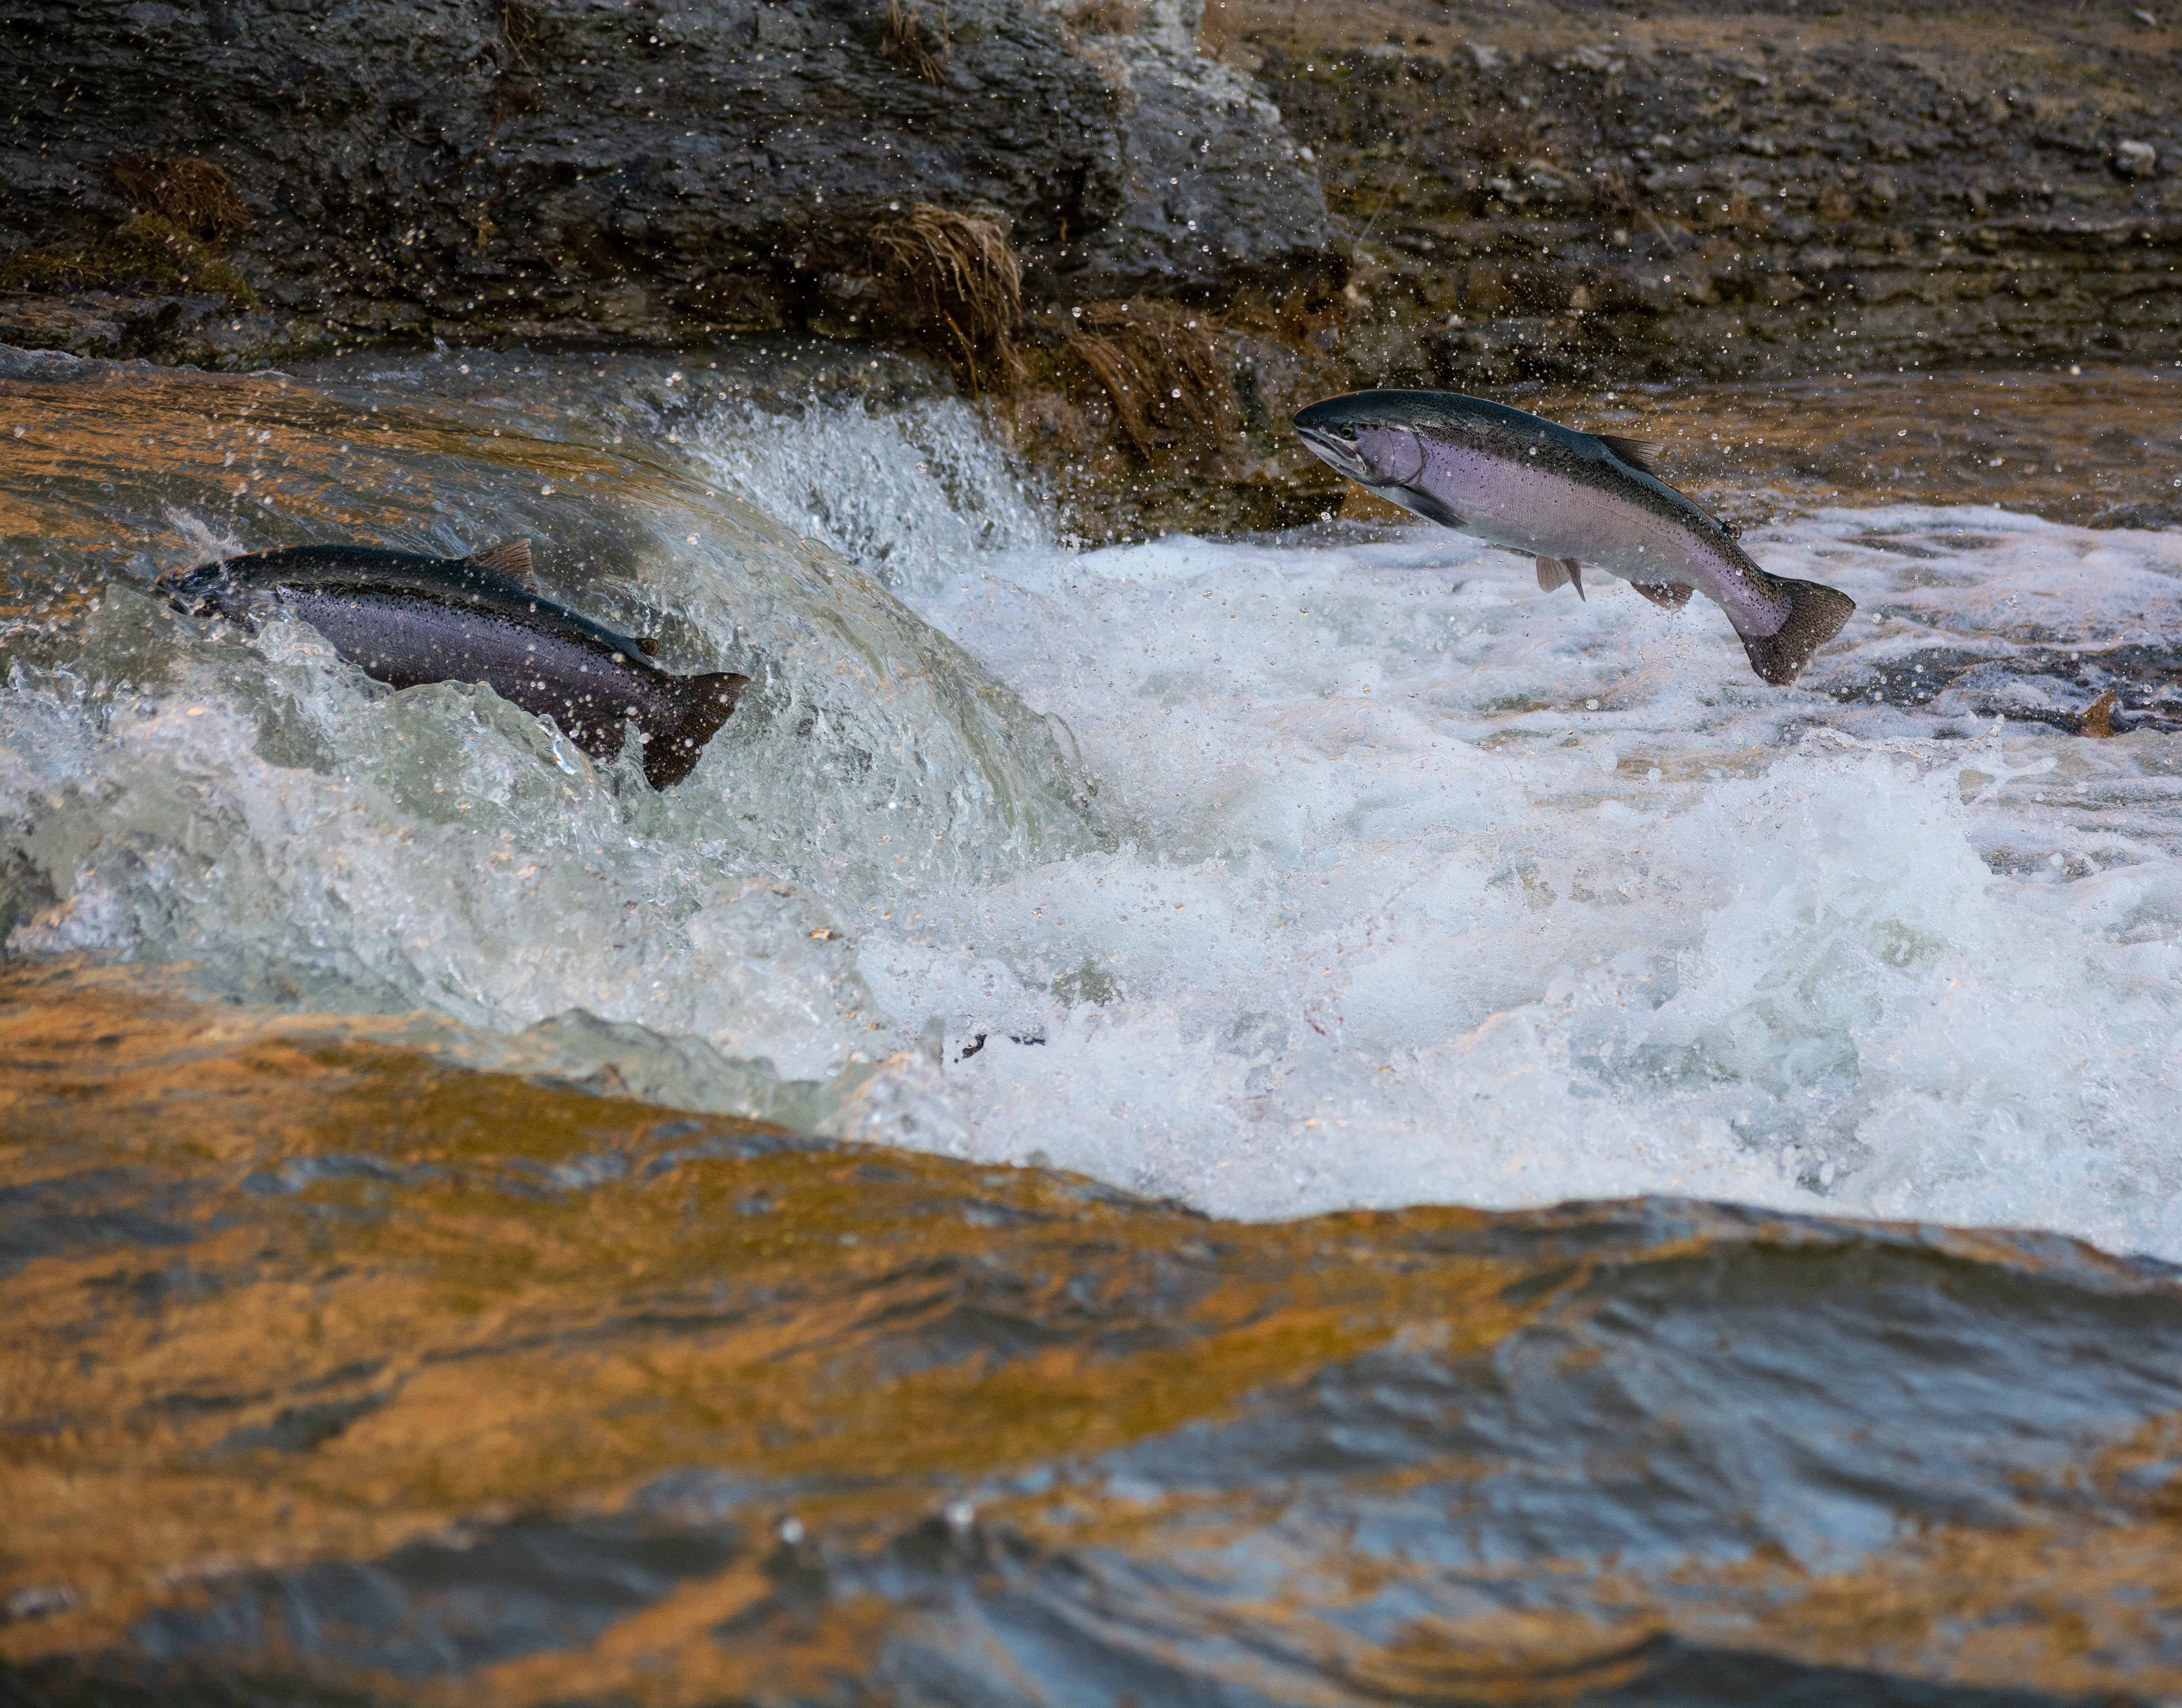
\includegraphics{spawn.jpg}

This plan represents the culmination of a collaborative planning process
undertaken in the Horsefly River watershed over many months of work with
a multi-partner planning team of individuals and groups passionate about
the conservation and restoration of freshwater ecosystems and the
species they support. Plan development was funded by the BC Salmon
Restoration and Innovation Fund, Canada Nature Fund for Aquatic Species
at Risk, and the RBC Bluewater Project. We were fortunate to benefit
from the feedback, guidance, and wisdom of many groups and individuals
who volunteered their time throughout this process --- this publication
would not have been possible without the engagement of our partners and
the planning team (see Table~\ref{tbl-planteam}).

We recognize the incredible fish passage and connectivity work that has
occurred in the Horsefly River watershed to date, and we are excited to
continue partnering with local groups and organizations to build upon
existing initiatives and provide a road map to push connectivity
restoration forward over the next 20 years and beyond.

The Canadian Wildlife Federation recognizes that the lands and waters
that form the basis of this plan are the traditional unceded territory
of the Northern Secwepemc people. We are grateful for the opportunity to
learn from the stewards of this land and work together to benefit
Pacific Salmon. A special thank you to Nishitha Singi for sharing the
traditional Secwepemctsín names used in this plan.

\bookmarksetup{startatroot}

\chapter*{Project Overview}\label{project-overview}
\addcontentsline{toc}{chapter}{Project Overview}

\markboth{Project Overview}{Project Overview}

\section*{Plan Purpose, Approach, and
Scope}\label{plan-purpose-approach-and-scope}
\addcontentsline{toc}{section}{Plan Purpose, Approach, and Scope}

\markright{Plan Purpose, Approach, and Scope}

The following Watershed Connectivity Restoration Plan (WCRP) represents
the culmination of a one-year collaborative planning effort, including
field assessments, the overall aim of which is to build collaborative
partnerships within the Horsefly River watershed to improve connectivity
for anadromous salmon and the livelihoods that they support, including
the continued sustenance, cultural, and ceremonial needs of the Northern
Secwépemc people. This 20-year plan was developed to identify priority
actions that the Horsefly River WCRP planning team (see
Table~\ref{tbl-planteam} for a list of team members) will undertake
between 2021-2040 to conserve and restore fish passage in the watershed,
through crossing rehabilitation, lateral barrier rehabilitation, dam
rehabilitation, and barrier prevention strategies.

WCRPs are long-term, actionable plans that blend local stakeholder and
rightsholder knowledge with innovative GIS analyses to gain a shared
understanding of where restoration efforts will have the greatest
benefit for anadromous salmon. The planning process is inspired by the
\href{https://cmp-openstandards.org/wp-content/uploads/2020/07/CMP-Open-Standards-for-the-Practice-of-Conservation-v4.0.pdf}{Conservation
Standards} (v.4.0), which is a conservation planning framework that
allows planning teams to systematically identify, implement, and monitor
strategies to apply the most effective solutions to high priority
conservation problems. There is a rich history of connectivity and fish
habitat planning and restoration work in the Horsefly River watershed
that this WCRP builds upon, including work undertaken by the BC Fish
Passage Technical Working Group, the Northern Secwepemc te Qelmucw
(NStQ) and member communities, the Horsefly River Roundtable, and other
local organizations (Ltd. (2018); S. Hocquard, Steve Hocquard
Consulting, pers. comm.).

The planning team compiled existing barrier location and assessment
data, habitat data, and previously identified priorities, and combined
this with local and Indigenous knowledge to create a strategic
watershed-scale plan to improve connectivity. To expand on this work the
Horsefly River WCRP planning team applied the WCRP planning framework to
define the ``thematic'' scope of freshwater connectivity and refine the
``geographic'' scope to identify only those portions of the watershed
where barrier prioritization will be conducted, and subsequent
restoration efforts will take place. Additionally, the team selected
target fish species, assessed their current connectivity status in the
watershed, defined concrete goals for gains in connectivity, and
developed a priority list of barriers for rehabilitation to achieve
those goals. While the current version of this plan is based on the
best-available information at the time of publishing, WCRPs are intended
to be ``living plans'' that are updated regularly as new information
becomes available, or if local priorities and contexts change. As such,
this document should be interpreted as a current snap-shot in time, and
future iterations of this WCRP will build upon the material presented in
this plan to continuously improve barrier rehabilitation for migratory
fish in the Horsefly River watershed. For more information on how WCRPs
are developed, see Mazany-Wright, Noseworthy, et al. (2021).

Field assessments were completed for 20 longitudinal barriers on the
preliminary barrier list during the summer of 2021, followed by a series
of WCRP Update Workshops in winter 2021. The aim of these workshops was
for the team to receive updates on progress made during the field
season, review assessment results and identify priority barriers, revise
the connectivity status assessment and goals, and update the Operational
Plan for 2022.

\section*{Vision Statement}\label{vision-statement}
\addcontentsline{toc}{section}{Vision Statement}

\markright{Vision Statement}

Healthy, well-connected streams and rivers within the Horsefly River
watershed support thriving populations of migratory fish, improving the
overall ecosystem health of the watershed. In turn, these fish provide
the continued sustenance, cultural, and ceremonial needs of the Northern
Secwépemc people, as they have since time immemorial. Both residents and
visitors to the watershed work together to mitigate the negative effects
of anthropogenic aquatic barriers, improving the resiliency of streams
and rivers for the benefit and appreciation of all.

\section*{Project Scope}\label{project-scope}
\addcontentsline{toc}{section}{Project Scope}

\markright{Project Scope}

Connectivity is a critical component of freshwater ecosystems that
encompasses a variety of factors related to ecosystem structure and
function, such as the ability of aquatic organisms to disperse and/or
migrate, the transportation of energy and matter (e.g., nutrient cycling
and sediment flows), and temperature regulation Seliger and Zeiringer
(2018). Though each of these factors are important when considering the
health of a watershed, for the purposes of this WCRP the term
``connectivity'' is defined as the degree to which aquatic organisms can
disperse and/or migrate freely through freshwater systems. Within this
context, connectivity is primarily constrained by physical barriers,
including anthropogenic infrastructure such as dams, weirs, and stream
crossings, and natural features such as waterfalls and debris flows.
This plan is intended to focus on the direct rehabilitation and
prevention of localized, physical barriers instead of the broad land-use
patterns that are causing chronic connectivity issues in the watershed.
The planning team decided that the primary focus of this WCRP is
addressing barriers to both longitudinal connectivity (i.e., along the
upstream-downstream plane) and lateral connectivity (i.e., connectivity
between the mainstem and adjacent riparian wetlands and floodplains) due
to the importance of maintaining fish passage to spawning, rearing, and
overwintering habitat in the watershed.

\begin{figure}

\centering{

\includegraphics{content/images/geo-scope-hors.png}

}

\caption{\label{fig-geoscope}The primary geographic scope --- the
Horsefly River watershed --- located in the Fraser River system.}

\end{figure}%

The primary geographic scope of this WCRP is the Horsefly River
watershed, located in the upper Fraser River drainage basin in central
British Columbia (Figure~\ref{fig-geoscope}). The scope constitutes the
Horsefly River ``watershed group'' as defined by the
\href{https://catalogue.data.gov.bc.ca/dataset/freshwater-atlas-watershed-groups}{British
Columbia Freshwater Atlas} (FWA). A consistent spatial framework was
necessary to undertake a watershed selection process at the provincial
scale to identify target watersheds to improve connectivity for salmon.
The Horsefly River watershed was identified by the BC Fish Passage
Restoration Initiative as one of four target watersheds for WCRP
development Mazany-Wright, Norris, et al. (2021b). The Horsefly River
watershed has a drainage area of 276,603 ha, spanning from the Quesnel
Highlands in the southeast to the confluence with Quesnel Lake in the
northwest. Culturally and economically important populations of Chinook
Salmon, Coho Salmon, and Sockeye Salmon are all found in the watershed,
which historically supported Indigenous sustenance and trading economies
(W. L. F. Nation. (2021), X. F. Nation. (2021)).

The Horsefly River watershed comprises parts of Secwepemcúl'ecw, the
traditional territory of the Northern Secwepemc te Qelmucw (NStQ),
represented by the Northern Shuswap Tribal Council and four member
communities or autonomous nations:

\begin{itemize}
\item
  Xatśūll Cmetem' (Soda Creek First Nations)
\item
  Stswēceḿc Xgāt'tem (Canoe Creek/Dog Creek First Nations)
\item
  T'ēxelc (Williams Lake First Nation)
\item
  Tsq'ēsceń (Canim Lake First Nation)
\end{itemize}

The geographic scope of this WCRP was further refined by identifying
``naturally accessible'' stream segments, which are defined as streams
that focal species should be able to access in the absence of
anthropogenic barriers (Figure~\ref{fig-strseg}). Naturally accessible
waterbodies were spatially delineated using fish species observation and
distribution data, as well as data on ``exclusionary points''. These
include waterfalls greater than 5 m in height, gradient barriers based
on species-specific swimming abilities, and watershed exclusion areas,
which are portions of the watershed where barrier rehabilitation efforts
should not occur. These maps were explored by the planning team to
incorporate additional local knowledge, ensure accuracy, and finalize
the constraints on naturally accessible waterbodies. The planning team
identified certain tributaries to the mainstem Horsefly River as
``watershed exclusion areas'', which were excluded from further
consideration under this plan, due to intermittent or insufficient flows
to support restoring connectivity for the focal species. The geographic
scope was further refined based on several confirmed impassable
waterfalls and modelled gradient barriers. Specifically, there are two
impassable waterfalls that severely limit naturally accessible habitat:
one on the mainstem Horsefly River approximately 4 km upstream of the
confluence with McKinley Creek, and the second on Moffat Creek
approximately 5 km upstream from where it flows into the Horsefly River.
All stream segments not identified as naturally accessible were removed
from the scope for further consideration. The ``constrained geographic
scope'' formed the foundation for all subsequent analyses and planning
steps, including mapping and modelling useable habitat types,
quantifying the current connectivity status, goal setting, and action
planning Mazany-Wright, Norris, et al. (2021a).

\begin{figure}

\centering{

\includegraphics{content/images/accessible-streams-hors.png}

}

\caption{\label{fig-strseg}Naturally accessible waterbodies within the
Horsefly River watershed. These do not represent useable habitat types,
but rather identifies the stream segments within which habitat modelling
and barrier mapping and prioritization was undertaken.}

\end{figure}%

\section*{Focal species}\label{focal-species}
\addcontentsline{toc}{section}{Focal species}

\markright{Focal species}

Focal species represent the ecologically and culturally important
species for which habitat connectivity is being conserved and/or
restored in the watershed. In the Horsefly River watershed, the planning
team selected Anadromous Salmon as the focal species group, which
comprises Chinook Salmon, Coho Salmon, and Sockeye Salmon. The selection
of these focal species was driven primarily by the targets species of
the primary fund supporting this planning work.

\subsection*{Anadromous Salmonids}\label{anadromous-salmonids}
\addcontentsline{toc}{subsection}{Anadromous Salmonids}

Anadromous salmon are cultural and ecological keystone species that
contribute to productive ecosystems by contributing marine-derived
nutrients to the watershed and forming an important food source for
other species. Salmon species are sacred to the NStQ, having sustained
life, trading economies, and culture since time immemorial (W. L. F.
Nation. (2021), X. F. Nation. (2021), N. Singi pers. comm.). The
stewardship of the resources and fisheries in their traditional
territories are imbued in the spirit of the NStQ through a symbiotic
relationship based on respect -- the NStQ never take more salmon than is
needed and there is no waste. The entirety of the salmon is used -
smoked and dried to sustain the NStQ through the winter months, the roe
harvested for consumption, salmon oil rendered to be stored and traded,
and the skin used to store the oil (Wilson, Twohig, and Dahlstrom
(1998), X. F. Nation. (2021), N. Singi pers. comm.). The salmon runs
begin to return to the Horsefly River watershed in early August, and the
NStQ traditionally celebrate and feast at this time. The harvest of the
salmon strengthens the cultural connection to the land and the waters,
providing an important food source for communities and the opportunity
to pass knowledge and ceremony to future generations through fishing and
fish processing (W. L. F. Nation. (2021)`, X. F. Nation. (2021)).

Anadromous salmon populations in the Horsefly River watershed have
declined significantly in the past few decades, with the populations of
all three focal species being listed as Threatened or Endangered by the
Committee On the Status of Endangered Wildlife In Canada (COSEWIC). This
has been exacerbated by the Big Bar landslide on the Fraser River in
2019, leading the four NStQ communities to voluntarily close the salmon
fishery from 2019-2022. The stewardship of their waters continues
through the work of the NStQ member communities and the Northern Shuswap
Tribal Council. See Appendix A for maps of modelled anadromous salmon
habitat in the Horsefly River Watershed.

\subsection*{Chinook Salmon \textbar{} Kekèsu \textbar{} Oncorhynchus
tshawytscha}\label{chinook-salmon-kekuxe8su-oncorhynchus-tshawytscha}
\addcontentsline{toc}{subsection}{Chinook Salmon \textbar{} Kekèsu
\textbar{} Oncorhynchus tshawytscha}

Chinook Salmon are the first to return each year, usually in early
August DFO (1991), and have the most limited distribution within the
watershed. Known spawning occurs in parts of the Horsefly River mainstem
above the confluence with the Little Horsefly River and throughout
McKinley Creek as far as Elbow Lake (DFO (1991), S. Hocquard, pers.
comm.). Important rearing systems include Patenaude Creek, Kroener
Creek, Black Creek, Woodjam Creek, Deerhorn Creek, and Wilmot Creek (S.
Hocquard, pers. comm.).

\subsection*{Coho Salmon \textbar{} Sxeyqs \textbar{} Oncorhynchus
kisutch}\label{coho-salmon-sxeyqs-oncorhynchus-kisutch}
\addcontentsline{toc}{subsection}{Coho Salmon \textbar{} Sxeyqs
\textbar{} Oncorhynchus kisutch}

Coho Salmon are the most widely distributed of the three focal species
in the watershed, with the ability to migrate into smaller, upper
tributary systems DFO (1991). Spawning occurs in the Little Horsefly
River between Gruhs Lake and Horsefly Lake, McKinley Creek below
McKinley Lake, Woodjam Creek, Patenaude Creek, Tisdall Creek, and Black
Creek. Rearing fry and juveniles have been observed in the Little
Horsefly River, Patenaude Creek, and McKinley Creek up to Bosk Lake (DFO
(1991), S. Hocquard pers. comm.).

\subsection*{Sockeye Salmon \textbar{} Sqlelten7ùwi \textbar{}
Oncorhynchus
nerka}\label{sockeye-salmon-sqlelten7uxf9wi-oncorhynchus-nerka}
\addcontentsline{toc}{subsection}{Sockeye Salmon \textbar{} Sqlelten7ùwi
\textbar{} Oncorhynchus nerka}

Sockeye Salmon have historically been the most abundant of the three
focal species in the watershed, though the population has seen
significant declines in recent years (DFO (1991), S. Hocquard pers.
comm.). Sockeye Salmon spawning is known to occur throughout the
Horsefly River (up to the impassable falls), in the Little Horsefly
River between Gruhs Lake and Horsefly Lake, Moffat Creek (up to the
impassible falls), and McKinley Creek up to Elbow Lake
(Pacific-Salmon-Foundation (2020), DFO (1991), S. Hocquard pers. comm.).
Additionally, a spawning channel aimed at enhancing the Sockeye Salmon
population was constructed by Fisheries and Oceans Canada in 1989 DFO
(1991). Currently, there are no Sockeye Salmon rearing in the Horsefly
River watershed -- all emergent fry migrate down to Quesnel Lake.

\section*{Barrier Types}\label{barrier-types}
\addcontentsline{toc}{section}{Barrier Types}

\markright{Barrier Types}

The following table highlights which barrier types pose the greatest
threat to anadromous salmon in the watershed. The results of this
assessment were used to inform the subsequent planning steps, as well as
to identify knowledge gaps where there is little spatial data to inform
the assessment for a specific barrier type.

\begin{longtable}[]{@{}lllll@{}}

\caption{\label{tbl-barriertype}Connectivity status assessment for (a)
linear habitat (spawning and rearing) and (b) overwintering habitat in
the Horsefly River watershed. The Available Habitat KEA is evaluated by
dividing the length of linear habitat that is currently accessible to
focal species by the total length of all linear habitat in the
watershed. The Available Overwintering Habitat KEA is evaluated as the
sum of all areal overwintering habitat that is accessible to focal
species.}

\tabularnewline

\caption{}\label{T_a803e}\tabularnewline
\toprule\noalign{}
Barrier Types & Extent & Severity & Irreversibility & Overall Threat
Rating: \\
\midrule\noalign{}
\endfirsthead
\toprule\noalign{}
Barrier Types & Extent & Severity & Irreversibility & Overall Threat
Rating: \\
\midrule\noalign{}
\endhead
\bottomrule\noalign{}
\endlastfoot
Road-Stream Crossings & Low & Low & Medium & Very High \\
Lateral Barriers & High & Very High & High & High \\
Small Dams(\textless3m height) & Low & Low & High & Medium \\
Trail-stream Crossings & Low & Low & Medium & Low \\
Natural Barriers & Medium & High & Low & Low \\

\end{longtable}

\subsection*{Small Dams (\textless3 m
height)}\label{small-dams-3-m-height}
\addcontentsline{toc}{subsection}{Small Dams (\textless3 m height)}

There are 6 mapped small dams on ``naturally accessible'' waterbodies in
the watershed, blocking a total of 1.42 km (\textasciitilde0.4\% of the
total habitat) of modelled spawning and rearing habitat for anadromous
salmon, resulting in a medium extent. The extent rating of these
structures was confirmed by the planning team. There are two known
fish-passage structures in the watershed, including on the dam at the
outlet of McKinley Lake. The remaining dams likely block passage for
anadromous salmon and would require significant resources to
rehabilitate. However, due to the limited extent of dams in the
watershed, a final pressure rating of Medium was assigned. Four small
dams were identified on the priority barrier list (see Appendix B).
Three of the dams require further assessment and confirmation of
upstream habitat quality, and the dam observed at the outlet of Kwun
Lake does not exist.

\subsection*{Road-stream Crossings}\label{road-stream-crossings}
\addcontentsline{toc}{subsection}{Road-stream Crossings}

Road-stream crossings are the most abundant barrier type in the
watershed, with 12 assessed and modelled crossings located on stream
segments with modelled habitat. Demographic road crossings (highways,
municipal, and paved roads) block 1.42 km of habitat (\textasciitilde0\%
of the total blocked habitat), with 0\% of assessed crossings having
been identified as barriers to fish passage. Resource roads block 1.42
km of habitat (\textasciitilde0\%), with 0\% of assessed crossings
having been identified as barriers. The planning team felt that the data
was underestimating the severity of road-stream crossing barriers in the
watershed, and therefore decided to update the rating from High to Very
High. The planning team also felt that an irreversibility rating of
Medium was appropriate due to the technical complexity and resources
required to rehabilitate road-stream crossings.

\subsection*{Trail-stream crossings}\label{trail-stream-crossings}
\addcontentsline{toc}{subsection}{Trail-stream crossings}

There is very little spatial data available on trail-stream crossings in
the watershed, so the planning team was unable to quantify the true
Extent and Severity of this barrier type. However, the planning team
felt that trail-stream crossings are not prevalent within the watershed
and that, where they do exist, they do not significantly impact passage
for anadromous salmon. As most crossings will be fords or similar
structures, rehabilitation may not be required, or rehabilitation costs
associated with these barriers would be quite low. Overall, the planning
team felt that the pressure rating for trail-stream crossings was likely
Low; however, the lack of ground-truthed evidence to support this rating
was identified as a knowledge gap within this plan.

\subsection*{Lateral Barriers}\label{lateral-barriers}
\addcontentsline{toc}{subsection}{Lateral Barriers}

There are numerous types of lateral barriers that potentially occur in
the watershed, including dykes, berms, and linear development (i.e.,
road and rail lines), all of which can restrict the ability of
anadromous salmon to move into floodplains, riparian wetlands, and other
off-channel habitats. No comprehensive lateral barrier data exists
within the watershed, so pressure ratings were based on qualitative
local knowledge. Lateral barriers are not thought to be as prevalent as
road- or rail-stream crossings but are likely very severe where they do
exist. Significant lateral barriers are known to occur along the
mainstem of the Horsefly River, which disconnect the mainstem river from
historic floodplain and off-channel habitat. Overall, the planning team
decided that a High pressure rating adequately captured the effect that
lateral barriers are having on connectivity in the watershed. Work to
begin quantifying and mapping lateral habitat will begin in 2022-23, as
described in the Operational Plan under Strategy 2: Lateral barrier
rehabilitation.

\subsection*{Natural Barriers}\label{natural-barriers}
\addcontentsline{toc}{subsection}{Natural Barriers}

Natural barriers to fish passage can include debris flows, log jams,
sediment deposits, etc., but natural features that have always
restricted fish passage (e.g., waterfalls) are not considered under this
barrier type. Natural barriers are difficult to include in a spatial
prioritization framework due to their transient nature. The planning
team identified known natural barriers that occur throughout the
watershed, such as beaver dams and log jams. Generally, these natural
barriers are only severe impediments to fish passage during low-flow
years, but reduced baseflows have become more common in recent years.
Based on this, the planning team felt that natural barriers will be
severe most years where they exist, but are mostly reversible, resulting
in an overall pressure rating of Low.

\bookmarksetup{startatroot}

\chapter*{Connectivity Status Assessment and
Goals}\label{connectivity-status-assessment-and-goals}
\addcontentsline{toc}{chapter}{Connectivity Status Assessment and Goals}

\markboth{Connectivity Status Assessment and Goals}{Connectivity Status
Assessment and Goals}

\section*{Connectivity Status
Assessment}\label{connectivity-status-assessment}
\addcontentsline{toc}{section}{Connectivity Status Assessment}

\markright{Connectivity Status Assessment}

The planning team identified two Key Ecological Attributes (KEAs) to
assess the current connectivity status of the watershed for each focal
species -- Accessible Habitat and Accessible Overwintering Habitat
(Table~\ref{tbl-connectivity}). KEAs are the key aspects of anadromous
salmon habitat that are being targeted by this WCRP. For each KEA, an
associated indicator was assigned to measure the status of that KEA. The
connectivity status indicators were used to establish goals to improve
key habitat connectivity over time and is the baseline against which
progress is tracked over time.

The current connectivity status was estimated using three spatial
models:

\begin{enumerate}
\def\labelenumi{\arabic{enumi}.}
\item
  Accessibility model: Naturally accessible waterbodies are those that
  are considered likely accessible to focal species if no human-made
  barriers existed on the landscape. These were spatially delineated for
  each focal species using natural barriers (i.e., waterfalls, gradient
  barriers, or subsurface flows) that would naturally limit upstream
  movement (Table~\ref{tbl-param}).
\item
  Habitat model: A subset of the naturally accessible waterbody layer
  was defined as key habitat, i.e., habitat likely to support spawning
  or rearing, rather than simply movement corridors. The habitat model
  identifies areas within waterbodies that have a higher potential to
  support key habitat based on stream channel gradient and discharge.
  The habitat model criteria can be found in (Table~\ref{tbl-param}).
\item
  Connectivity model: A layer of known or modelled structures was
  overlaid on the key habitat results. Structures with unknown
  passability were treated as a full barrier until confirmed passable by
  either local knowledge, desktop review, or field assessment. Watershed
  connectivity was estimated by calculating the amount of key habitat
  that is connected to the ocean (i.e., not fragmented by human-made
  barriers). Key habitat with no structures or only passable structures
  downstream was considered connected. Key habitat upstream of full,
  partial, or potential barriers was considered disconnected. All
  connected habitat was summed and divided by the total amount of key
  habitat in the watershed to arrive at the KEA indicators. Detailed
  methods for the connectivity model can be found in Appendix C.
\end{enumerate}

\begin{longtable}[]{@{}lllllll@{}}

\caption{\label{tbl-connectivity}Connectivity status assessment for
spawning (a) and rearing (b) habitat in the Bulkley River watershed. The
two KEAs - Accessible Spawning Habitat and Accessible Rearing Habitat -
are evaluated by dividing the length of linear habitat (of each type)
that is currently accessible to focal species by the total length of all
linear habitat (of each type) in the watershed.}

\tabularnewline

\caption{}\label{T_07072}\tabularnewline
\toprule\noalign{}
Focal Species & KEA & Indicator & Poor & Fair & Good & Very Good \\
\midrule\noalign{}
\endfirsthead
\toprule\noalign{}
Focal Species & KEA & Indicator & Poor & Fair & Good & Very Good \\
\midrule\noalign{}
\endhead
\bottomrule\noalign{}
\endlastfoot
Andromous Salmon & Available Habitat & \% of total linear habitat &
\textless80\% & - & 81-90\% & \textgreater90\% \\
& & Current Status: & & & & 92 \\

\end{longtable}

\textbf{Comments:} Indicator rating definitions are based on the
consensus decisions of the planning team, including the decision not to
define Fair. The current status is based on the CWF Barrier
Prioritization Model output, which is current as of March 2022.

\begin{longtable}[]{@{}lllllll@{}}
\caption{}\label{T_30c3a}\tabularnewline
\toprule\noalign{}
Focal Species & KEA & Indicator & Poor & Fair & Good & Very Good \\
\midrule\noalign{}
\endfirsthead
\toprule\noalign{}
Focal Species & KEA & Indicator & Poor & Fair & Good & Very Good \\
\midrule\noalign{}
\endhead
\bottomrule\noalign{}
\endlastfoot
Andromous Salmon & Available Overwintering Habitat & Total Area (m2) of
overwintering habitat accessible & ? & ? & ? & ? \\
& & Current Status: & & & & \\
\end{longtable}

\textbf{Comments:} No baseline data exists on the extent of
overwintering habitat in the watershed. A priority action is included in
the Operational Plan (strategy 2.3) to develop a habitat layer, and this
will be used to inform this connectivity status assessment in the
future.

\section*{Goals}\label{goals}
\addcontentsline{toc}{section}{Goals}

\markright{Goals}

\begin{longtable}[]{@{}ll@{}}

\caption{\label{tbl-goals}Goals to improve (1) spawning and rearing and
(2) overwintering habitat connectivity for focal species in the Horsefly
River watershed over the lifespan of the WCRP (2021-2040). The goals
were established through discussions with the planning team and
represent the resulting desired state of connectivity in the watershed.
The goals are subject to change as more information and data are
collected over the course of the plan timeline (e.g., the current
connectivity status is updated based on barrier field assessments).}

\tabularnewline

\caption{}\label{T_fa550}\tabularnewline
\toprule\noalign{}
Goal \# & Goal \\
\midrule\noalign{}
\endfirsthead
\toprule\noalign{}
Goal \# & Goal \\
\midrule\noalign{}
\endhead
\bottomrule\noalign{}
\endlastfoot
1 & By 2040, the percent (\%) of total linear habitat accessible to
anadromous salmon will increase from 92\% to 96\% within the Horsefly
River watershed (i.e., reconnect at least 14.77 km of habitat). \\
2 & By 2024, the total area of overwintering habitat accessible to
Anadromous Salmon will increase by 1,500 m2 within the Horsefly River
watershed. \\

\end{longtable}

\bookmarksetup{startatroot}

\chapter*{Structure Prioritization}\label{structure-prioritization}
\addcontentsline{toc}{chapter}{Structure Prioritization}

\markboth{Structure Prioritization}{Structure Prioritization}

\section*{Horsefly River Watershed Structure Prioritization
Summary}\label{horsefly-river-watershed-structure-prioritization-summary}
\addcontentsline{toc}{section}{Horsefly River Watershed Structure
Prioritization Summary}

\markright{Horsefly River Watershed Structure Prioritization Summary}

A primary outcome of the WCRP will be the rehabilitation of barriers to
connectivity in the Horsefly River watershed. To achieve the goals in
this plan, it is necessary to identify a suite of barriers that, if
rehabilitated, will provide access to a minimum of 14.77 key habitat
(Table~\ref{tbl-table16}).

\begin{longtable}[]{@{}llllll@{}}

\caption{\label{tbl-table16}Spawning and rearing habitat connectivity
gain requirements to meet WCRP goals in the Horsefly River watershed.
The measures of currently accessible and total habitat values are
derived from the Intrinsic Potential habitat model described in Appendix
B.}

\tabularnewline

\caption{}\label{T_2622f}\tabularnewline
\toprule\noalign{}
Habitat Type & Currently accessible (km) & Total & Current Connectivity
Status & Goal & Gain required (km) \\
\midrule\noalign{}
\endfirsthead
\toprule\noalign{}
Habitat Type & Currently accessible (km) & Total & Current Connectivity
Status & Goal & Gain required (km) \\
\midrule\noalign{}
\endhead
\bottomrule\noalign{}
\endlastfoot
Spawning and Rearing & 326.28 & 355.26 & 92\% & 96\% & 14.77 \\

\end{longtable}

After all existing data and knowledge are collated for known and
modelled crossings, an iterative ranking process is conducted to help
confirm barriers to target for rehabilitation to meet the goals. The
ranking process is primarily used to guide field assessments and
maximize efficiency in ground truthing data inputs and model outputs,
while providing a secondary purpose to evaluate the relative key habitat
gains of confirmed barriers in the watershed. This process, combined
with input from local knowledge holders and experts, is used to develop
field plans for assessing barriers that have the potential to block the
most key habitat in the watershed. Field assessments are based on the BC
Fish Passage Strategic Approach Envrionment (2014) and can include a
barrier assessment (i.e., evaluating passability of the structure), a
habitat confirmation (i.e., evaluation of whether the upstream habitat
is suitable for the focal species and whether there are other
undocumented anthropogenic or natural barriers upstream or downstream),
or a detailed habitat investigation (e.g., a fish passage study or
further in-depth analysis of habitat features in a waterbody). The
ranking process accounts for the long-term and immediate potential
habitat gains potentially offered by each structure to identify
structures that maximize long-term and immediate potential to improve
key habitat connectivity in the watershed. All structures in the
watershed (excluding those confirmed as passable) are ranked in each
iteration of the ranking process. Details of the ranking process used to
guide field assessments can be found in
\href{supplimentary-information.qmd}{Appendix B}.

\section*{Structure Prioritzation
Summary}\label{structure-prioritzation-summary}
\addcontentsline{toc}{section}{Structure Prioritzation Summary}

\markright{Structure Prioritzation Summary}

Following field assessments, structures are placed on one of five
possible lists:

\begin{enumerate}
\def\labelenumi{\arabic{enumi}.}
\item
  Priority barriers list -- the structure is confirmed as a full or
  partial barrier, has key habitat confirmed to exist upstream, and is
  considered actionable by the planning team (i.e., action items will be
  identified to advance rehabilitation of the structure). Depending on
  the barrier, owner, financial constraints, and quality of upstream
  habitat, the action may be to leave to end of life cycle before
  reviewing again, remove and decommission the road, replace with a new
  passable structure, or modify to temporarily restore connectivity
  (e.g., fish ladder or baffles installed; (Table~\ref{tbl-priority})).
\item
  Assessed structures that remain data deficient list -- some form of
  field assessment has been completed on the structure, but further
  investigation is required to confirm either the passability status or
  presence/suitability of upstream habitat (Table~\ref{tbl-deficient}).
\item
  Rehabilitated barriers list -- priority barriers that have been
  addressed (either through removal, replacement, or temporary fish
  passage improvement projects; (Table~\ref{tbl-rehab}))
\item
  Non-actionable barriers list -- the structure is confirmed to be a
  barrier to fish passage and have some amount/quality of habitat
  upstream, but the planning team will not identify actions to advance
  rehabilitation of the structure because of logistic considerations
  (e.g., financial costs), short habitat gain, or the upstream habitat
  is of poor quality or unsuitable in its present condition to support
  key life stages of the focal species \href{data-methods.qmd}{Appendix
  C}.
\item
  Excluded structures list -- the structure is excluded from further
  consideration in subsequent ranking and work planning because the
  structure is confirmed passable (e.g., bridge), not present, or there
  is no key habitat upstream \href{data-methods.qmd}{Appendix C}.
\end{enumerate}

\global\setlength{\Oldarrayrulewidth}{\arrayrulewidth}

\global\setlength{\Oldtabcolsep}{\tabcolsep}

\setlength{\tabcolsep}{2pt}

\renewcommand*{\arraystretch}{1.5}



\providecommand{\ascline}[3]{\noalign{\global\arrayrulewidth #1}\arrayrulecolor[HTML]{#2}\cline{#3}}

\begin{longtable}[c]{|p{0.93in}|p{1.76in}|p{1.86in}|p{2.25in}|p{1.84in}|p{1.50in}|p{1.38in}|p{1.47in}|p{1.58in}|p{1.99in}|p{1.48in}|p{2.54in}|p{6.25in}|p{12.84in}|p{5.84in}}

\caption{\label{tbl-priority}The Horsefly River watershed priority
barrier list, which includes barriers that have undergone field
assessment, been reviewed by the planning team, and selected to pursue
for proactive rehabilitation.}

\tabularnewline

\hhline{>{\arrayrulecolor[HTML]{666666}\global\arrayrulewidth=1.5pt}->{\arrayrulecolor[HTML]{666666}\global\arrayrulewidth=1.5pt}->{\arrayrulecolor[HTML]{666666}\global\arrayrulewidth=1.5pt}->{\arrayrulecolor[HTML]{666666}\global\arrayrulewidth=1.5pt}->{\arrayrulecolor[HTML]{666666}\global\arrayrulewidth=1.5pt}->{\arrayrulecolor[HTML]{666666}\global\arrayrulewidth=1.5pt}->{\arrayrulecolor[HTML]{666666}\global\arrayrulewidth=1.5pt}->{\arrayrulecolor[HTML]{666666}\global\arrayrulewidth=1.5pt}->{\arrayrulecolor[HTML]{666666}\global\arrayrulewidth=1.5pt}->{\arrayrulecolor[HTML]{666666}\global\arrayrulewidth=1.5pt}->{\arrayrulecolor[HTML]{666666}\global\arrayrulewidth=1.5pt}->{\arrayrulecolor[HTML]{666666}\global\arrayrulewidth=1.5pt}->{\arrayrulecolor[HTML]{666666}\global\arrayrulewidth=1.5pt}->{\arrayrulecolor[HTML]{666666}\global\arrayrulewidth=1.5pt}->{\arrayrulecolor[HTML]{666666}\global\arrayrulewidth=1.5pt}-}

\multicolumn{1}{>{\cellcolor[HTML]{008270}\raggedright}m{\dimexpr 0.93in+0\tabcolsep}}{\textcolor[HTML]{FFFFFF}{\fontsize{11}{11}\selectfont{\global\setmainfont{Arial}{barrier\_id}}}} & \multicolumn{1}{>{\cellcolor[HTML]{008270}\raggedright}m{\dimexpr 1.76in+0\tabcolsep}}{\textcolor[HTML]{FFFFFF}{\fontsize{11}{11}\selectfont{\global\setmainfont{Arial}{modelled\_crossing\_id}}}} & \multicolumn{1}{>{\cellcolor[HTML]{008270}\raggedright}m{\dimexpr 1.86in+0\tabcolsep}}{\textcolor[HTML]{FFFFFF}{\fontsize{11}{11}\selectfont{\global\setmainfont{Arial}{watercourse\_name}}}} & \multicolumn{1}{>{\cellcolor[HTML]{008270}\raggedright}m{\dimexpr 2.25in+0\tabcolsep}}{\textcolor[HTML]{FFFFFF}{\fontsize{11}{11}\selectfont{\global\setmainfont{Arial}{road\_name}}}} & \multicolumn{1}{>{\cellcolor[HTML]{008270}\raggedright}m{\dimexpr 1.84in+0\tabcolsep}}{\textcolor[HTML]{FFFFFF}{\fontsize{11}{11}\selectfont{\global\setmainfont{Arial}{structure\_type}}}} & \multicolumn{1}{>{\cellcolor[HTML]{008270}\raggedright}m{\dimexpr 1.5in+0\tabcolsep}}{\textcolor[HTML]{FFFFFF}{\fontsize{11}{11}\selectfont{\global\setmainfont{Arial}{partial\_passability}}}} & \multicolumn{1}{>{\cellcolor[HTML]{008270}\raggedright}m{\dimexpr 1.38in+0\tabcolsep}}{\textcolor[HTML]{FFFFFF}{\fontsize{11}{11}\selectfont{\global\setmainfont{Arial}{structure\_owner}}}} & \multicolumn{1}{>{\cellcolor[HTML]{008270}\raggedright}m{\dimexpr 1.47in+0\tabcolsep}}{\textcolor[HTML]{FFFFFF}{\fontsize{11}{11}\selectfont{\global\setmainfont{Arial}{num\_barriers\_set}}}} & \multicolumn{1}{>{\cellcolor[HTML]{008270}\raggedright}m{\dimexpr 1.58in+0\tabcolsep}}{\textcolor[HTML]{FFFFFF}{\fontsize{11}{11}\selectfont{\global\setmainfont{Arial}{total\_hab\_gain\_set}}}} & \multicolumn{1}{>{\cellcolor[HTML]{008270}\raggedright}m{\dimexpr 1.99in+0\tabcolsep}}{\textcolor[HTML]{FFFFFF}{\fontsize{11}{11}\selectfont{\global\setmainfont{Arial}{upstream\_habitat\_quality}}}} & \multicolumn{1}{>{\cellcolor[HTML]{008270}\raggedright}m{\dimexpr 1.48in+0\tabcolsep}}{\textcolor[HTML]{FFFFFF}{\fontsize{11}{11}\selectfont{\global\setmainfont{Arial}{estimated\_cost\_\$}}}} & \multicolumn{1}{>{\cellcolor[HTML]{008270}\raggedright}m{\dimexpr 2.54in+0\tabcolsep}}{\textcolor[HTML]{FFFFFF}{\fontsize{11}{11}\selectfont{\global\setmainfont{Arial}{next\_steps}}}} & \multicolumn{1}{>{\cellcolor[HTML]{008270}\raggedright}m{\dimexpr 6.25in+0\tabcolsep}}{\textcolor[HTML]{FFFFFF}{\fontsize{11}{11}\selectfont{\global\setmainfont{Arial}{reason}}}} & \multicolumn{1}{>{\cellcolor[HTML]{008270}\raggedright}m{\dimexpr 12.84in+0\tabcolsep}}{\textcolor[HTML]{FFFFFF}{\fontsize{11}{11}\selectfont{\global\setmainfont{Arial}{notes}}}} & \multicolumn{1}{>{\cellcolor[HTML]{008270}\raggedright}m{\dimexpr 5.84in+0\tabcolsep}}{\textcolor[HTML]{FFFFFF}{\fontsize{11}{11}\selectfont{\global\setmainfont{Arial}{supporting\_links}}}} \\

\noalign{\global\arrayrulewidth 0pt}\arrayrulecolor[HTML]{000000}

\hhline{>{\arrayrulecolor[HTML]{666666}\global\arrayrulewidth=1.5pt}->{\arrayrulecolor[HTML]{666666}\global\arrayrulewidth=1.5pt}->{\arrayrulecolor[HTML]{666666}\global\arrayrulewidth=1.5pt}->{\arrayrulecolor[HTML]{666666}\global\arrayrulewidth=1.5pt}->{\arrayrulecolor[HTML]{666666}\global\arrayrulewidth=1.5pt}->{\arrayrulecolor[HTML]{666666}\global\arrayrulewidth=1.5pt}->{\arrayrulecolor[HTML]{666666}\global\arrayrulewidth=1.5pt}->{\arrayrulecolor[HTML]{666666}\global\arrayrulewidth=1.5pt}->{\arrayrulecolor[HTML]{666666}\global\arrayrulewidth=1.5pt}->{\arrayrulecolor[HTML]{666666}\global\arrayrulewidth=1.5pt}->{\arrayrulecolor[HTML]{666666}\global\arrayrulewidth=1.5pt}->{\arrayrulecolor[HTML]{666666}\global\arrayrulewidth=1.5pt}->{\arrayrulecolor[HTML]{666666}\global\arrayrulewidth=1.5pt}->{\arrayrulecolor[HTML]{666666}\global\arrayrulewidth=1.5pt}->{\arrayrulecolor[HTML]{666666}\global\arrayrulewidth=1.5pt}-}\endfirsthead 

\hhline{>{\arrayrulecolor[HTML]{666666}\global\arrayrulewidth=1.5pt}->{\arrayrulecolor[HTML]{666666}\global\arrayrulewidth=1.5pt}->{\arrayrulecolor[HTML]{666666}\global\arrayrulewidth=1.5pt}->{\arrayrulecolor[HTML]{666666}\global\arrayrulewidth=1.5pt}->{\arrayrulecolor[HTML]{666666}\global\arrayrulewidth=1.5pt}->{\arrayrulecolor[HTML]{666666}\global\arrayrulewidth=1.5pt}->{\arrayrulecolor[HTML]{666666}\global\arrayrulewidth=1.5pt}->{\arrayrulecolor[HTML]{666666}\global\arrayrulewidth=1.5pt}->{\arrayrulecolor[HTML]{666666}\global\arrayrulewidth=1.5pt}->{\arrayrulecolor[HTML]{666666}\global\arrayrulewidth=1.5pt}->{\arrayrulecolor[HTML]{666666}\global\arrayrulewidth=1.5pt}->{\arrayrulecolor[HTML]{666666}\global\arrayrulewidth=1.5pt}->{\arrayrulecolor[HTML]{666666}\global\arrayrulewidth=1.5pt}->{\arrayrulecolor[HTML]{666666}\global\arrayrulewidth=1.5pt}->{\arrayrulecolor[HTML]{666666}\global\arrayrulewidth=1.5pt}-}

\multicolumn{1}{>{\cellcolor[HTML]{008270}\raggedright}m{\dimexpr 0.93in+0\tabcolsep}}{\textcolor[HTML]{FFFFFF}{\fontsize{11}{11}\selectfont{\global\setmainfont{Arial}{barrier\_id}}}} & \multicolumn{1}{>{\cellcolor[HTML]{008270}\raggedright}m{\dimexpr 1.76in+0\tabcolsep}}{\textcolor[HTML]{FFFFFF}{\fontsize{11}{11}\selectfont{\global\setmainfont{Arial}{modelled\_crossing\_id}}}} & \multicolumn{1}{>{\cellcolor[HTML]{008270}\raggedright}m{\dimexpr 1.86in+0\tabcolsep}}{\textcolor[HTML]{FFFFFF}{\fontsize{11}{11}\selectfont{\global\setmainfont{Arial}{watercourse\_name}}}} & \multicolumn{1}{>{\cellcolor[HTML]{008270}\raggedright}m{\dimexpr 2.25in+0\tabcolsep}}{\textcolor[HTML]{FFFFFF}{\fontsize{11}{11}\selectfont{\global\setmainfont{Arial}{road\_name}}}} & \multicolumn{1}{>{\cellcolor[HTML]{008270}\raggedright}m{\dimexpr 1.84in+0\tabcolsep}}{\textcolor[HTML]{FFFFFF}{\fontsize{11}{11}\selectfont{\global\setmainfont{Arial}{structure\_type}}}} & \multicolumn{1}{>{\cellcolor[HTML]{008270}\raggedright}m{\dimexpr 1.5in+0\tabcolsep}}{\textcolor[HTML]{FFFFFF}{\fontsize{11}{11}\selectfont{\global\setmainfont{Arial}{partial\_passability}}}} & \multicolumn{1}{>{\cellcolor[HTML]{008270}\raggedright}m{\dimexpr 1.38in+0\tabcolsep}}{\textcolor[HTML]{FFFFFF}{\fontsize{11}{11}\selectfont{\global\setmainfont{Arial}{structure\_owner}}}} & \multicolumn{1}{>{\cellcolor[HTML]{008270}\raggedright}m{\dimexpr 1.47in+0\tabcolsep}}{\textcolor[HTML]{FFFFFF}{\fontsize{11}{11}\selectfont{\global\setmainfont{Arial}{num\_barriers\_set}}}} & \multicolumn{1}{>{\cellcolor[HTML]{008270}\raggedright}m{\dimexpr 1.58in+0\tabcolsep}}{\textcolor[HTML]{FFFFFF}{\fontsize{11}{11}\selectfont{\global\setmainfont{Arial}{total\_hab\_gain\_set}}}} & \multicolumn{1}{>{\cellcolor[HTML]{008270}\raggedright}m{\dimexpr 1.99in+0\tabcolsep}}{\textcolor[HTML]{FFFFFF}{\fontsize{11}{11}\selectfont{\global\setmainfont{Arial}{upstream\_habitat\_quality}}}} & \multicolumn{1}{>{\cellcolor[HTML]{008270}\raggedright}m{\dimexpr 1.48in+0\tabcolsep}}{\textcolor[HTML]{FFFFFF}{\fontsize{11}{11}\selectfont{\global\setmainfont{Arial}{estimated\_cost\_\$}}}} & \multicolumn{1}{>{\cellcolor[HTML]{008270}\raggedright}m{\dimexpr 2.54in+0\tabcolsep}}{\textcolor[HTML]{FFFFFF}{\fontsize{11}{11}\selectfont{\global\setmainfont{Arial}{next\_steps}}}} & \multicolumn{1}{>{\cellcolor[HTML]{008270}\raggedright}m{\dimexpr 6.25in+0\tabcolsep}}{\textcolor[HTML]{FFFFFF}{\fontsize{11}{11}\selectfont{\global\setmainfont{Arial}{reason}}}} & \multicolumn{1}{>{\cellcolor[HTML]{008270}\raggedright}m{\dimexpr 12.84in+0\tabcolsep}}{\textcolor[HTML]{FFFFFF}{\fontsize{11}{11}\selectfont{\global\setmainfont{Arial}{notes}}}} & \multicolumn{1}{>{\cellcolor[HTML]{008270}\raggedright}m{\dimexpr 5.84in+0\tabcolsep}}{\textcolor[HTML]{FFFFFF}{\fontsize{11}{11}\selectfont{\global\setmainfont{Arial}{supporting\_links}}}} \\

\noalign{\global\arrayrulewidth 0pt}\arrayrulecolor[HTML]{000000}

\hhline{>{\arrayrulecolor[HTML]{666666}\global\arrayrulewidth=1.5pt}->{\arrayrulecolor[HTML]{666666}\global\arrayrulewidth=1.5pt}->{\arrayrulecolor[HTML]{666666}\global\arrayrulewidth=1.5pt}->{\arrayrulecolor[HTML]{666666}\global\arrayrulewidth=1.5pt}->{\arrayrulecolor[HTML]{666666}\global\arrayrulewidth=1.5pt}->{\arrayrulecolor[HTML]{666666}\global\arrayrulewidth=1.5pt}->{\arrayrulecolor[HTML]{666666}\global\arrayrulewidth=1.5pt}->{\arrayrulecolor[HTML]{666666}\global\arrayrulewidth=1.5pt}->{\arrayrulecolor[HTML]{666666}\global\arrayrulewidth=1.5pt}->{\arrayrulecolor[HTML]{666666}\global\arrayrulewidth=1.5pt}->{\arrayrulecolor[HTML]{666666}\global\arrayrulewidth=1.5pt}->{\arrayrulecolor[HTML]{666666}\global\arrayrulewidth=1.5pt}->{\arrayrulecolor[HTML]{666666}\global\arrayrulewidth=1.5pt}->{\arrayrulecolor[HTML]{666666}\global\arrayrulewidth=1.5pt}->{\arrayrulecolor[HTML]{666666}\global\arrayrulewidth=1.5pt}-}\endhead



\multicolumn{1}{>{\raggedright}m{\dimexpr 0.93in+0\tabcolsep}}{\textcolor[HTML]{000000}{\fontsize{11}{11}\selectfont{\global\setmainfont{Arial}{124150}}}} & \multicolumn{1}{>{\raggedright}m{\dimexpr 1.76in+0\tabcolsep}}{\textcolor[HTML]{000000}{\fontsize{11}{11}\selectfont{\global\setmainfont{Arial}{6800503}}}} & \multicolumn{1}{>{\raggedright}m{\dimexpr 1.86in+0\tabcolsep}}{\textcolor[HTML]{000000}{\fontsize{11}{11}\selectfont{\global\setmainfont{Arial}{Trib\ to\ Deerhorn}}}} & \multicolumn{1}{>{\raggedright}m{\dimexpr 2.25in+0\tabcolsep}}{\textcolor[HTML]{000000}{\fontsize{11}{11}\selectfont{\global\setmainfont{Arial}{unnamed}}}} & \multicolumn{1}{>{\raggedright}m{\dimexpr 1.84in+0\tabcolsep}}{\textcolor[HTML]{000000}{\fontsize{11}{11}\selectfont{\global\setmainfont{Arial}{Stream\ crossing\ -\ CBS}}}} & \multicolumn{1}{>{\raggedright}m{\dimexpr 1.5in+0\tabcolsep}}{\textcolor[HTML]{000000}{\fontsize{11}{11}\selectfont{\global\setmainfont{Arial}{Unknown}}}} & \multicolumn{1}{>{\raggedright}m{\dimexpr 1.38in+0\tabcolsep}}{\textcolor[HTML]{000000}{\fontsize{11}{11}\selectfont{\global\setmainfont{Arial}{Private}}}} & \multicolumn{1}{>{\raggedright}m{\dimexpr 1.47in+0\tabcolsep}}{\textcolor[HTML]{000000}{\fontsize{11}{11}\selectfont{\global\setmainfont{Arial}{1}}}} & \multicolumn{1}{>{\raggedright}m{\dimexpr 1.58in+0\tabcolsep}}{\textcolor[HTML]{000000}{\fontsize{11}{11}\selectfont{\global\setmainfont{Arial}{1.89}}}} & \multicolumn{1}{>{\raggedright}m{\dimexpr 1.99in+0\tabcolsep}}{\textcolor[HTML]{000000}{\fontsize{11}{11}\selectfont{\global\setmainfont{Arial}{High}}}} & \multicolumn{1}{>{\raggedright}m{\dimexpr 1.48in+0\tabcolsep}}{\textcolor[HTML]{000000}{\fontsize{11}{11}\selectfont{\global\setmainfont{Arial}{150000}}}} & \multicolumn{1}{>{\raggedright}m{\dimexpr 2.54in+0\tabcolsep}}{\textcolor[HTML]{000000}{\fontsize{11}{11}\selectfont{\global\setmainfont{Arial}{Engage\ with\ barrier\ owner}}}} & \multicolumn{1}{>{\raggedright}m{\dimexpr 6.25in+0\tabcolsep}}{\textcolor[HTML]{000000}{\fontsize{11}{11}\selectfont{\global\setmainfont{Arial}{Undersized\ culvert,\ fish\ present}}}} & \multicolumn{1}{>{\raggedright}m{\dimexpr 12.84in+0\tabcolsep}}{\textcolor[HTML]{000000}{\fontsize{11}{11}\selectfont{\global\setmainfont{Arial}{Landowner\ says\ fish\ present}}}} & \multicolumn{1}{>{\raggedright}m{\dimexpr 5.84in+0\tabcolsep}}{\textcolor[HTML]{000000}{\fontsize{11}{11}\selectfont{\global\setmainfont{Arial}{http://a100.gov.bc.ca/pub/pscismap/imageViewer.do?assessmentId=124330\ }}}} \\

\noalign{\global\arrayrulewidth 0pt}\arrayrulecolor[HTML]{000000}





\multicolumn{1}{>{\raggedright}m{\dimexpr 0.93in+0\tabcolsep}}{\textcolor[HTML]{000000}{\fontsize{11}{11}\selectfont{\global\setmainfont{Arial}{124249}}}} & \multicolumn{1}{>{\raggedright}m{\dimexpr 1.76in+0\tabcolsep}}{\textcolor[HTML]{000000}{\fontsize{11}{11}\selectfont{\global\setmainfont{Arial}{6800023}}}} & \multicolumn{1}{>{\raggedright}m{\dimexpr 1.86in+0\tabcolsep}}{\textcolor[HTML]{000000}{\fontsize{11}{11}\selectfont{\global\setmainfont{Arial}{Wawn\ Lake\ Creek}}}} & \multicolumn{1}{>{\raggedright}m{\dimexpr 2.25in+0\tabcolsep}}{\textcolor[HTML]{000000}{\fontsize{11}{11}\selectfont{\global\setmainfont{Arial}{Millar\ Road}}}} & \multicolumn{1}{>{\raggedright}m{\dimexpr 1.84in+0\tabcolsep}}{\textcolor[HTML]{000000}{\fontsize{11}{11}\selectfont{\global\setmainfont{Arial}{Stream\ crossing\ -\ CBS}}}} & \multicolumn{1}{>{\raggedright}m{\dimexpr 1.5in+0\tabcolsep}}{\textcolor[HTML]{000000}{\fontsize{11}{11}\selectfont{\global\setmainfont{Arial}{Unknown}}}} & \multicolumn{1}{>{\raggedright}m{\dimexpr 1.38in+0\tabcolsep}}{\textcolor[HTML]{000000}{\fontsize{11}{11}\selectfont{\global\setmainfont{Arial}{MOTI}}}} & \multicolumn{1}{>{\raggedright}m{\dimexpr 1.47in+0\tabcolsep}}{\textcolor[HTML]{000000}{\fontsize{11}{11}\selectfont{\global\setmainfont{Arial}{1}}}} & \multicolumn{1}{>{\raggedright}m{\dimexpr 1.58in+0\tabcolsep}}{\textcolor[HTML]{000000}{\fontsize{11}{11}\selectfont{\global\setmainfont{Arial}{0.70}}}} & \multicolumn{1}{>{\raggedright}m{\dimexpr 1.99in+0\tabcolsep}}{\textcolor[HTML]{000000}{\fontsize{11}{11}\selectfont{\global\setmainfont{Arial}{Medium}}}} & \multicolumn{1}{>{\raggedright}m{\dimexpr 1.48in+0\tabcolsep}}{\textcolor[HTML]{000000}{\fontsize{11}{11}\selectfont{\global\setmainfont{Arial}{400000}}}} & \multicolumn{1}{>{\raggedright}m{\dimexpr 2.54in+0\tabcolsep}}{\textcolor[HTML]{000000}{\fontsize{11}{11}\selectfont{\global\setmainfont{Arial}{Engage\ with\ barrier\ owner}}}} & \multicolumn{1}{>{\raggedright}m{\dimexpr 6.25in+0\tabcolsep}}{\textcolor[HTML]{000000}{\fontsize{11}{11}\selectfont{\global\setmainfont{Arial}{Deferred\ until\ Vedder\ and\ Wilmot\ complete}}}} & \multicolumn{1}{>{\raggedright}m{\dimexpr 12.84in+0\tabcolsep}}{\textcolor[HTML]{000000}{\fontsize{11}{11}\selectfont{\global\setmainfont{Arial}{Currently\ backwatered\ by\ impassable\ beaver\ dam.\ Undersized}}}} & \multicolumn{1}{>{\raggedright}m{\dimexpr 5.84in+0\tabcolsep}}{\textcolor[HTML]{000000}{\fontsize{11}{11}\selectfont{\global\setmainfont{Arial}{http://a100.gov.bc.ca/pub/pscismap/imageViewer.do?habitatConfirmationId=1882\ }}}} \\

\noalign{\global\arrayrulewidth 0pt}\arrayrulecolor[HTML]{000000}





\multicolumn{1}{>{\raggedright}m{\dimexpr 0.93in+0\tabcolsep}}{\textcolor[HTML]{000000}{\fontsize{11}{11}\selectfont{\global\setmainfont{Arial}{124256}}}} & \multicolumn{1}{>{\raggedright}m{\dimexpr 1.76in+0\tabcolsep}}{\textcolor[HTML]{000000}{\fontsize{11}{11}\selectfont{\global\setmainfont{Arial}{6800022}}}} & \multicolumn{1}{>{\raggedright}m{\dimexpr 1.86in+0\tabcolsep}}{\textcolor[HTML]{000000}{\fontsize{11}{11}\selectfont{\global\setmainfont{Arial}{Harpers\ Creek}}}} & \multicolumn{1}{>{\raggedright}m{\dimexpr 2.25in+0\tabcolsep}}{\textcolor[HTML]{000000}{\fontsize{11}{11}\selectfont{\global\setmainfont{Arial}{Horsefly\ Road}}}} & \multicolumn{1}{>{\raggedright}m{\dimexpr 1.84in+0\tabcolsep}}{\textcolor[HTML]{000000}{\fontsize{11}{11}\selectfont{\global\setmainfont{Arial}{Stream\ crossing\ -\ CBS}}}} & \multicolumn{1}{>{\raggedright}m{\dimexpr 1.5in+0\tabcolsep}}{\textcolor[HTML]{000000}{\fontsize{11}{11}\selectfont{\global\setmainfont{Arial}{No}}}} & \multicolumn{1}{>{\raggedright}m{\dimexpr 1.38in+0\tabcolsep}}{\textcolor[HTML]{000000}{\fontsize{11}{11}\selectfont{\global\setmainfont{Arial}{MOTI}}}} & \multicolumn{1}{>{\raggedright}m{\dimexpr 1.47in+0\tabcolsep}}{\textcolor[HTML]{000000}{\fontsize{11}{11}\selectfont{\global\setmainfont{Arial}{2}}}} & \multicolumn{1}{>{\raggedright}m{\dimexpr 1.58in+0\tabcolsep}}{\textcolor[HTML]{000000}{\fontsize{11}{11}\selectfont{\global\setmainfont{Arial}{0.69}}}} & \multicolumn{1}{>{\raggedright}m{\dimexpr 1.99in+0\tabcolsep}}{\textcolor[HTML]{000000}{\fontsize{11}{11}\selectfont{\global\setmainfont{Arial}{Medium}}}} & \multicolumn{1}{>{\raggedright}m{\dimexpr 1.48in+0\tabcolsep}}{\textcolor[HTML]{000000}{\fontsize{11}{11}\selectfont{\global\setmainfont{Arial}{400000}}}} & \multicolumn{1}{>{\raggedright}m{\dimexpr 2.54in+0\tabcolsep}}{\textcolor[HTML]{000000}{\fontsize{11}{11}\selectfont{\global\setmainfont{Arial}{Commission\ engineering\ designs}}}} & \multicolumn{1}{>{\raggedright}m{\dimexpr 6.25in+0\tabcolsep}}{\textcolor[HTML]{000000}{\fontsize{11}{11}\selectfont{\global\setmainfont{Arial}{Decent\ rearing\ habitat\ in\ Harpers\ Lake}}}} & \multicolumn{1}{>{\raggedright}m{\dimexpr 12.84in+0\tabcolsep}}{\textcolor[HTML]{000000}{\fontsize{11}{11}\selectfont{\global\setmainfont{Arial}{Designs\ on\ hold\ while\ Vedder\ and\ Wilmot\ addressed}}}} & \multicolumn{1}{>{\raggedright}m{\dimexpr 5.84in+0\tabcolsep}}{\textcolor[HTML]{000000}{\fontsize{11}{11}\selectfont{\global\setmainfont{Arial}{http://a100.gov.bc.ca/pub/pscismap/imageViewer.do?habitatConfirmationId=1883\ }}}} \\

\noalign{\global\arrayrulewidth 0pt}\arrayrulecolor[HTML]{000000}





\multicolumn{1}{>{\raggedright}m{\dimexpr 0.93in+0\tabcolsep}}{\textcolor[HTML]{000000}{\fontsize{11}{11}\selectfont{\global\setmainfont{Arial}{124268}}}} & \multicolumn{1}{>{\raggedright}m{\dimexpr 1.76in+0\tabcolsep}}{\textcolor[HTML]{000000}{\fontsize{11}{11}\selectfont{\global\setmainfont{Arial}{6800048}}}} & \multicolumn{1}{>{\raggedright}m{\dimexpr 1.86in+0\tabcolsep}}{\textcolor[HTML]{000000}{\fontsize{11}{11}\selectfont{\global\setmainfont{Arial}{Vedder\ Creek}}}} & \multicolumn{1}{>{\raggedright}m{\dimexpr 2.25in+0\tabcolsep}}{\textcolor[HTML]{000000}{\fontsize{11}{11}\selectfont{\global\setmainfont{Arial}{Horsefly-Quesnel\ Lake\ Road}}}} & \multicolumn{1}{>{\raggedright}m{\dimexpr 1.84in+0\tabcolsep}}{\textcolor[HTML]{000000}{\fontsize{11}{11}\selectfont{\global\setmainfont{Arial}{Stream\ crossing\ -\ CBS}}}} & \multicolumn{1}{>{\raggedright}m{\dimexpr 1.5in+0\tabcolsep}}{\textcolor[HTML]{000000}{\fontsize{11}{11}\selectfont{\global\setmainfont{Arial}{Yes}}}} & \multicolumn{1}{>{\raggedright}m{\dimexpr 1.38in+0\tabcolsep}}{\textcolor[HTML]{000000}{\fontsize{11}{11}\selectfont{\global\setmainfont{Arial}{MOTI}}}} & \multicolumn{1}{>{\raggedright}m{\dimexpr 1.47in+0\tabcolsep}}{\textcolor[HTML]{000000}{\fontsize{11}{11}\selectfont{\global\setmainfont{Arial}{2}}}} & \multicolumn{1}{>{\raggedright}m{\dimexpr 1.58in+0\tabcolsep}}{\textcolor[HTML]{000000}{\fontsize{11}{11}\selectfont{\global\setmainfont{Arial}{0.87}}}} & \multicolumn{1}{>{\raggedright}m{\dimexpr 1.99in+0\tabcolsep}}{\textcolor[HTML]{000000}{\fontsize{11}{11}\selectfont{\global\setmainfont{Arial}{High}}}} & \multicolumn{1}{>{\raggedright}m{\dimexpr 1.48in+0\tabcolsep}}{\textcolor[HTML]{000000}{\fontsize{11}{11}\selectfont{\global\setmainfont{Arial}{400000}}}} & \multicolumn{1}{>{\raggedright}m{\dimexpr 2.54in+0\tabcolsep}}{\textcolor[HTML]{000000}{\fontsize{11}{11}\selectfont{\global\setmainfont{Arial}{Commission\ engineering\ designs}}}} & \multicolumn{1}{>{\raggedright}m{\dimexpr 6.25in+0\tabcolsep}}{\textcolor[HTML]{000000}{\fontsize{11}{11}\selectfont{\global\setmainfont{Arial}{Salmonid\ juveniles\ observed\ indicating\ high\ quality\ habitat}}}} & \multicolumn{1}{>{\raggedright}m{\dimexpr 12.84in+0\tabcolsep}}{\textcolor[HTML]{000000}{\fontsize{11}{11}\selectfont{\global\setmainfont{Arial}{Designs\ in\ progress}}}} & \multicolumn{1}{>{\raggedright}m{\dimexpr 5.84in+0\tabcolsep}}{\textcolor[HTML]{000000}{\fontsize{11}{11}\selectfont{\global\setmainfont{Arial}{http://a100.gov.bc.ca/pub/pscismap/imageViewer.do?assessmentId=124448\ }}}} \\

\noalign{\global\arrayrulewidth 0pt}\arrayrulecolor[HTML]{000000}





\multicolumn{1}{>{\raggedright}m{\dimexpr 0.93in+0\tabcolsep}}{\textcolor[HTML]{000000}{\fontsize{11}{11}\selectfont{\global\setmainfont{Arial}{124272}}}} & \multicolumn{1}{>{\raggedright}m{\dimexpr 1.76in+0\tabcolsep}}{\textcolor[HTML]{000000}{\fontsize{11}{11}\selectfont{\global\setmainfont{Arial}{}}}} & \multicolumn{1}{>{\raggedright}m{\dimexpr 1.86in+0\tabcolsep}}{\textcolor[HTML]{000000}{\fontsize{11}{11}\selectfont{\global\setmainfont{Arial}{Trib\ to\ Woodjam\ Creek}}}} & \multicolumn{1}{>{\raggedright}m{\dimexpr 2.25in+0\tabcolsep}}{\textcolor[HTML]{000000}{\fontsize{11}{11}\selectfont{\global\setmainfont{Arial}{Unnamed}}}} & \multicolumn{1}{>{\raggedright}m{\dimexpr 1.84in+0\tabcolsep}}{\textcolor[HTML]{000000}{\fontsize{11}{11}\selectfont{\global\setmainfont{Arial}{Stream\ crossing\ -\ CBS}}}} & \multicolumn{1}{>{\raggedright}m{\dimexpr 1.5in+0\tabcolsep}}{\textcolor[HTML]{000000}{\fontsize{11}{11}\selectfont{\global\setmainfont{Arial}{Yes}}}} & \multicolumn{1}{>{\raggedright}m{\dimexpr 1.38in+0\tabcolsep}}{\textcolor[HTML]{000000}{\fontsize{11}{11}\selectfont{\global\setmainfont{Arial}{Private\ }}}} & \multicolumn{1}{>{\raggedright}m{\dimexpr 1.47in+0\tabcolsep}}{\textcolor[HTML]{000000}{\fontsize{11}{11}\selectfont{\global\setmainfont{Arial}{1}}}} & \multicolumn{1}{>{\raggedright}m{\dimexpr 1.58in+0\tabcolsep}}{\textcolor[HTML]{000000}{\fontsize{11}{11}\selectfont{\global\setmainfont{Arial}{1.15}}}} & \multicolumn{1}{>{\raggedright}m{\dimexpr 1.99in+0\tabcolsep}}{\textcolor[HTML]{000000}{\fontsize{11}{11}\selectfont{\global\setmainfont{Arial}{High}}}} & \multicolumn{1}{>{\raggedright}m{\dimexpr 1.48in+0\tabcolsep}}{\textcolor[HTML]{000000}{\fontsize{11}{11}\selectfont{\global\setmainfont{Arial}{150000}}}} & \multicolumn{1}{>{\raggedright}m{\dimexpr 2.54in+0\tabcolsep}}{\textcolor[HTML]{000000}{\fontsize{11}{11}\selectfont{\global\setmainfont{Arial}{Engage\ with\ barrier\ owner}}}} & \multicolumn{1}{>{\raggedright}m{\dimexpr 6.25in+0\tabcolsep}}{\textcolor[HTML]{000000}{\fontsize{11}{11}\selectfont{\global\setmainfont{Arial}{Undersized\ culvert,\ fish\ present}}}} & \multicolumn{1}{>{\raggedright}m{\dimexpr 12.84in+0\tabcolsep}}{\textcolor[HTML]{000000}{\fontsize{11}{11}\selectfont{\global\setmainfont{Arial}{abundant\ fish\ downstream\ during\ 2017\ assessment.\ May\ be\ passable\ to\ adults}}}} & \multicolumn{1}{>{\raggedright}m{\dimexpr 5.84in+0\tabcolsep}}{\textcolor[HTML]{000000}{\fontsize{11}{11}\selectfont{\global\setmainfont{Arial}{http://a100.gov.bc.ca/pub/pscismap/imageViewer.do?assessmentId=197823\ }}}} \\

\noalign{\global\arrayrulewidth 0pt}\arrayrulecolor[HTML]{000000}





\multicolumn{1}{>{\raggedright}m{\dimexpr 0.93in+0\tabcolsep}}{\textcolor[HTML]{000000}{\fontsize{11}{11}\selectfont{\global\setmainfont{Arial}{126471}}}} & \multicolumn{1}{>{\raggedright}m{\dimexpr 1.76in+0\tabcolsep}}{\textcolor[HTML]{000000}{\fontsize{11}{11}\selectfont{\global\setmainfont{Arial}{}}}} & \multicolumn{1}{>{\raggedright}m{\dimexpr 1.86in+0\tabcolsep}}{\textcolor[HTML]{000000}{\fontsize{11}{11}\selectfont{\global\setmainfont{Arial}{Trib\ to\ Woodjam\ Creek}}}} & \multicolumn{1}{>{\raggedright}m{\dimexpr 2.25in+0\tabcolsep}}{\textcolor[HTML]{000000}{\fontsize{11}{11}\selectfont{\global\setmainfont{Arial}{unnamed}}}} & \multicolumn{1}{>{\raggedright}m{\dimexpr 1.84in+0\tabcolsep}}{\textcolor[HTML]{000000}{\fontsize{11}{11}\selectfont{\global\setmainfont{Arial}{Stream\ crossing\ -\ CBS}}}} & \multicolumn{1}{>{\raggedright}m{\dimexpr 1.5in+0\tabcolsep}}{\textcolor[HTML]{000000}{\fontsize{11}{11}\selectfont{\global\setmainfont{Arial}{Yes}}}} & \multicolumn{1}{>{\raggedright}m{\dimexpr 1.38in+0\tabcolsep}}{\textcolor[HTML]{000000}{\fontsize{11}{11}\selectfont{\global\setmainfont{Arial}{FLNRO}}}} & \multicolumn{1}{>{\raggedright}m{\dimexpr 1.47in+0\tabcolsep}}{\textcolor[HTML]{000000}{\fontsize{11}{11}\selectfont{\global\setmainfont{Arial}{1}}}} & \multicolumn{1}{>{\raggedright}m{\dimexpr 1.58in+0\tabcolsep}}{\textcolor[HTML]{000000}{\fontsize{11}{11}\selectfont{\global\setmainfont{Arial}{0.10}}}} & \multicolumn{1}{>{\raggedright}m{\dimexpr 1.99in+0\tabcolsep}}{\textcolor[HTML]{000000}{\fontsize{11}{11}\selectfont{\global\setmainfont{Arial}{Medium}}}} & \multicolumn{1}{>{\raggedright}m{\dimexpr 1.48in+0\tabcolsep}}{\textcolor[HTML]{000000}{\fontsize{11}{11}\selectfont{\global\setmainfont{Arial}{20000}}}} & \multicolumn{1}{>{\raggedright}m{\dimexpr 2.54in+0\tabcolsep}}{\textcolor[HTML]{000000}{\fontsize{11}{11}\selectfont{\global\setmainfont{Arial}{Engage\ with\ barrier\ owner}}}} & \multicolumn{1}{>{\raggedright}m{\dimexpr 6.25in+0\tabcolsep}}{\textcolor[HTML]{000000}{\fontsize{11}{11}\selectfont{\global\setmainfont{Arial}{Potentially\ easy\ fix}}}} & \multicolumn{1}{>{\raggedright}m{\dimexpr 12.84in+0\tabcolsep}}{\textcolor[HTML]{000000}{\fontsize{11}{11}\selectfont{\global\setmainfont{Arial}{Cattle\ trail,\ may\ be\ able\ to\ decommission\ or\ replace\ with\ small\ 3\ m\ bridge.\ Discuss\ with\ barrier\ owner.\ Short\ habitat\ gain,\ parr\ able\ to\ pass\ at\ some\ flows,\ dewatering/\ stranding\ potential.}}}} & \multicolumn{1}{>{\raggedright}m{\dimexpr 5.84in+0\tabcolsep}}{\textcolor[HTML]{000000}{\fontsize{11}{11}\selectfont{\global\setmainfont{Arial}{http://a100.gov.bc.ca/pub/pscismap/imageViewer.do?habitatConfirmationId=685\ }}}} \\

\noalign{\global\arrayrulewidth 0pt}\arrayrulecolor[HTML]{000000}





\multicolumn{1}{>{\raggedright}m{\dimexpr 0.93in+0\tabcolsep}}{\textcolor[HTML]{000000}{\fontsize{11}{11}\selectfont{\global\setmainfont{Arial}{197762}}}} & \multicolumn{1}{>{\raggedright}m{\dimexpr 1.76in+0\tabcolsep}}{\textcolor[HTML]{000000}{\fontsize{11}{11}\selectfont{\global\setmainfont{Arial}{6800487}}}} & \multicolumn{1}{>{\raggedright}m{\dimexpr 1.86in+0\tabcolsep}}{\textcolor[HTML]{000000}{\fontsize{11}{11}\selectfont{\global\setmainfont{Arial}{Divan\ Creek}}}} & \multicolumn{1}{>{\raggedright}m{\dimexpr 2.25in+0\tabcolsep}}{\textcolor[HTML]{000000}{\fontsize{11}{11}\selectfont{\global\setmainfont{Arial}{unnamed}}}} & \multicolumn{1}{>{\raggedright}m{\dimexpr 1.84in+0\tabcolsep}}{\textcolor[HTML]{000000}{\fontsize{11}{11}\selectfont{\global\setmainfont{Arial}{Stream\ crossing\ -\ Ford}}}} & \multicolumn{1}{>{\raggedright}m{\dimexpr 1.5in+0\tabcolsep}}{\textcolor[HTML]{000000}{\fontsize{11}{11}\selectfont{\global\setmainfont{Arial}{No}}}} & \multicolumn{1}{>{\raggedright}m{\dimexpr 1.38in+0\tabcolsep}}{\textcolor[HTML]{000000}{\fontsize{11}{11}\selectfont{\global\setmainfont{Arial}{Forest\ tenure}}}} & \multicolumn{1}{>{\raggedright}m{\dimexpr 1.47in+0\tabcolsep}}{\textcolor[HTML]{000000}{\fontsize{11}{11}\selectfont{\global\setmainfont{Arial}{1}}}} & \multicolumn{1}{>{\raggedright}m{\dimexpr 1.58in+0\tabcolsep}}{\textcolor[HTML]{000000}{\fontsize{11}{11}\selectfont{\global\setmainfont{Arial}{1.44}}}} & \multicolumn{1}{>{\raggedright}m{\dimexpr 1.99in+0\tabcolsep}}{\textcolor[HTML]{000000}{\fontsize{11}{11}\selectfont{\global\setmainfont{Arial}{Low}}}} & \multicolumn{1}{>{\raggedright}m{\dimexpr 1.48in+0\tabcolsep}}{\textcolor[HTML]{000000}{\fontsize{11}{11}\selectfont{\global\setmainfont{Arial}{2000}}}} & \multicolumn{1}{>{\raggedright}m{\dimexpr 2.54in+0\tabcolsep}}{\textcolor[HTML]{000000}{\fontsize{11}{11}\selectfont{\global\setmainfont{Arial}{Engage\ with\ barrier\ owner}}}} & \multicolumn{1}{>{\raggedright}m{\dimexpr 6.25in+0\tabcolsep}}{\textcolor[HTML]{000000}{\fontsize{11}{11}\selectfont{\global\setmainfont{Arial}{Industry\ barrier}}}} & \multicolumn{1}{>{\raggedright}m{\dimexpr 12.84in+0\tabcolsep}}{\textcolor[HTML]{000000}{\fontsize{11}{11}\selectfont{\global\setmainfont{Arial}{No\ permitted\ roads\ to\ site.\ Talk\ to\ Tolko\ about\ potential\ hand\ removal}}}} & \multicolumn{1}{>{\raggedright}m{\dimexpr 5.84in+0\tabcolsep}}{\textcolor[HTML]{000000}{\fontsize{11}{11}\selectfont{\global\setmainfont{Arial}{http://a100.gov.bc.ca/pub/pscismap/imageViewer.do?assessmentId=198782\ }}}} \\

\noalign{\global\arrayrulewidth 0pt}\arrayrulecolor[HTML]{000000}





\multicolumn{1}{>{\raggedright}m{\dimexpr 0.93in+0\tabcolsep}}{\textcolor[HTML]{000000}{\fontsize{11}{11}\selectfont{\global\setmainfont{Arial}{198300}}}} & \multicolumn{1}{>{\raggedright}m{\dimexpr 1.76in+0\tabcolsep}}{\textcolor[HTML]{000000}{\fontsize{11}{11}\selectfont{\global\setmainfont{Arial}{6800483}}}} & \multicolumn{1}{>{\raggedright}m{\dimexpr 1.86in+0\tabcolsep}}{\textcolor[HTML]{000000}{\fontsize{11}{11}\selectfont{\global\setmainfont{Arial}{Molybdenite\ Creek}}}} & \multicolumn{1}{>{\raggedright}m{\dimexpr 2.25in+0\tabcolsep}}{\textcolor[HTML]{000000}{\fontsize{11}{11}\selectfont{\global\setmainfont{Arial}{West\ Fraser/Tolko}}}} & \multicolumn{1}{>{\raggedright}m{\dimexpr 1.84in+0\tabcolsep}}{\textcolor[HTML]{000000}{\fontsize{11}{11}\selectfont{\global\setmainfont{Arial}{Stream\ crossing\ -\ Ford}}}} & \multicolumn{1}{>{\raggedright}m{\dimexpr 1.5in+0\tabcolsep}}{\textcolor[HTML]{000000}{\fontsize{11}{11}\selectfont{\global\setmainfont{Arial}{Unknown}}}} & \multicolumn{1}{>{\raggedright}m{\dimexpr 1.38in+0\tabcolsep}}{\textcolor[HTML]{000000}{\fontsize{11}{11}\selectfont{\global\setmainfont{Arial}{Forest\ tenure}}}} & \multicolumn{1}{>{\raggedright}m{\dimexpr 1.47in+0\tabcolsep}}{\textcolor[HTML]{000000}{\fontsize{11}{11}\selectfont{\global\setmainfont{Arial}{1}}}} & \multicolumn{1}{>{\raggedright}m{\dimexpr 1.58in+0\tabcolsep}}{\textcolor[HTML]{000000}{\fontsize{11}{11}\selectfont{\global\setmainfont{Arial}{0.88}}}} & \multicolumn{1}{>{\raggedright}m{\dimexpr 1.99in+0\tabcolsep}}{\textcolor[HTML]{000000}{\fontsize{11}{11}\selectfont{\global\setmainfont{Arial}{High}}}} & \multicolumn{1}{>{\raggedright}m{\dimexpr 1.48in+0\tabcolsep}}{\textcolor[HTML]{000000}{\fontsize{11}{11}\selectfont{\global\setmainfont{Arial}{10000}}}} & \multicolumn{1}{>{\raggedright}m{\dimexpr 2.54in+0\tabcolsep}}{\textcolor[HTML]{000000}{\fontsize{11}{11}\selectfont{\global\setmainfont{Arial}{Engage\ with\ barrier\ owner}}}} & \multicolumn{1}{>{\raggedright}m{\dimexpr 6.25in+0\tabcolsep}}{\textcolor[HTML]{000000}{\fontsize{11}{11}\selectfont{\global\setmainfont{Arial}{Industry\ barrier}}}} & \multicolumn{1}{>{\raggedright}m{\dimexpr 12.84in+0\tabcolsep}}{\textcolor[HTML]{000000}{\fontsize{11}{11}\selectfont{\global\setmainfont{Arial}{Remove\ debris\ from\ collapsed\ bridge\ from\ stream\ channel.\ Currently\ a\ barrier\ at\ low\ flows}}}} & \multicolumn{1}{>{\raggedright}m{\dimexpr 5.84in+0\tabcolsep}}{\textcolor[HTML]{000000}{\fontsize{11}{11}\selectfont{\global\setmainfont{Arial}{http://a100.gov.bc.ca/pub/pscismap/imageViewer.do?assessmentId=199520\ }}}} \\

\noalign{\global\arrayrulewidth 0pt}\arrayrulecolor[HTML]{000000}





\multicolumn{1}{>{\raggedright}m{\dimexpr 0.93in+0\tabcolsep}}{\textcolor[HTML]{000000}{\fontsize{11}{11}\selectfont{\global\setmainfont{Arial}{198876}}}} & \multicolumn{1}{>{\raggedright}m{\dimexpr 1.76in+0\tabcolsep}}{\textcolor[HTML]{000000}{\fontsize{11}{11}\selectfont{\global\setmainfont{Arial}{}}}} & \multicolumn{1}{>{\raggedright}m{\dimexpr 1.86in+0\tabcolsep}}{\textcolor[HTML]{000000}{\fontsize{11}{11}\selectfont{\global\setmainfont{Arial}{Vedder\ Creek}}}} & \multicolumn{1}{>{\raggedright}m{\dimexpr 2.25in+0\tabcolsep}}{\textcolor[HTML]{000000}{\fontsize{11}{11}\selectfont{\global\setmainfont{Arial}{Private}}}} & \multicolumn{1}{>{\raggedright}m{\dimexpr 1.84in+0\tabcolsep}}{\textcolor[HTML]{000000}{\fontsize{11}{11}\selectfont{\global\setmainfont{Arial}{Stream\ crossing\ -\ CBS}}}} & \multicolumn{1}{>{\raggedright}m{\dimexpr 1.5in+0\tabcolsep}}{\textcolor[HTML]{000000}{\fontsize{11}{11}\selectfont{\global\setmainfont{Arial}{Yes}}}} & \multicolumn{1}{>{\raggedright}m{\dimexpr 1.38in+0\tabcolsep}}{\textcolor[HTML]{000000}{\fontsize{11}{11}\selectfont{\global\setmainfont{Arial}{Private\ }}}} & \multicolumn{1}{>{\raggedright}m{\dimexpr 1.47in+0\tabcolsep}}{\textcolor[HTML]{000000}{\fontsize{11}{11}\selectfont{\global\setmainfont{Arial}{2}}}} & \multicolumn{1}{>{\raggedright}m{\dimexpr 1.58in+0\tabcolsep}}{\textcolor[HTML]{000000}{\fontsize{11}{11}\selectfont{\global\setmainfont{Arial}{0.87}}}} & \multicolumn{1}{>{\raggedright}m{\dimexpr 1.99in+0\tabcolsep}}{\textcolor[HTML]{000000}{\fontsize{11}{11}\selectfont{\global\setmainfont{Arial}{High}}}} & \multicolumn{1}{>{\raggedright}m{\dimexpr 1.48in+0\tabcolsep}}{\textcolor[HTML]{000000}{\fontsize{11}{11}\selectfont{\global\setmainfont{Arial}{2000}}}} & \multicolumn{1}{>{\raggedright}m{\dimexpr 2.54in+0\tabcolsep}}{\textcolor[HTML]{000000}{\fontsize{11}{11}\selectfont{\global\setmainfont{Arial}{Engage\ with\ barrier\ owner}}}} & \multicolumn{1}{>{\raggedright}m{\dimexpr 6.25in+0\tabcolsep}}{\textcolor[HTML]{000000}{\fontsize{11}{11}\selectfont{\global\setmainfont{Arial}{Easy\ fix,\ high\ quality\ habitat}}}} & \multicolumn{1}{>{\raggedright}m{\dimexpr 12.84in+0\tabcolsep}}{\textcolor[HTML]{000000}{\fontsize{11}{11}\selectfont{\global\setmainfont{Arial}{Small\ flexi\ culvert,\ likely\ could\ be\ removed\ by\ hand}}}} & \multicolumn{1}{>{\raggedright}m{\dimexpr 5.84in+0\tabcolsep}}{\textcolor[HTML]{000000}{\fontsize{11}{11}\selectfont{\global\setmainfont{Arial}{http://a100.gov.bc.ca/pub/pscismap/imageViewer.do?assessmentId=200136\ }}}} \\

\noalign{\global\arrayrulewidth 0pt}\arrayrulecolor[HTML]{000000}





\multicolumn{1}{>{\raggedright}m{\dimexpr 0.93in+0\tabcolsep}}{\textcolor[HTML]{000000}{\fontsize{11}{11}\selectfont{\global\setmainfont{Arial}{57158}}}} & \multicolumn{1}{>{\raggedright}m{\dimexpr 1.76in+0\tabcolsep}}{\textcolor[HTML]{000000}{\fontsize{11}{11}\selectfont{\global\setmainfont{Arial}{6800596}}}} & \multicolumn{1}{>{\raggedright}m{\dimexpr 1.86in+0\tabcolsep}}{\textcolor[HTML]{000000}{\fontsize{11}{11}\selectfont{\global\setmainfont{Arial}{Trib\ to\ McKinley\ Creek}}}} & \multicolumn{1}{>{\raggedright}m{\dimexpr 2.25in+0\tabcolsep}}{\textcolor[HTML]{000000}{\fontsize{11}{11}\selectfont{\global\setmainfont{Arial}{R02156-887}}}} & \multicolumn{1}{>{\raggedright}m{\dimexpr 1.84in+0\tabcolsep}}{\textcolor[HTML]{000000}{\fontsize{11}{11}\selectfont{\global\setmainfont{Arial}{Stream\ crossing\ -\ CBS}}}} & \multicolumn{1}{>{\raggedright}m{\dimexpr 1.5in+0\tabcolsep}}{\textcolor[HTML]{000000}{\fontsize{11}{11}\selectfont{\global\setmainfont{Arial}{No}}}} & \multicolumn{1}{>{\raggedright}m{\dimexpr 1.38in+0\tabcolsep}}{\textcolor[HTML]{000000}{\fontsize{11}{11}\selectfont{\global\setmainfont{Arial}{Forest\ tenure}}}} & \multicolumn{1}{>{\raggedright}m{\dimexpr 1.47in+0\tabcolsep}}{\textcolor[HTML]{000000}{\fontsize{11}{11}\selectfont{\global\setmainfont{Arial}{2}}}} & \multicolumn{1}{>{\raggedright}m{\dimexpr 1.58in+0\tabcolsep}}{\textcolor[HTML]{000000}{\fontsize{11}{11}\selectfont{\global\setmainfont{Arial}{0.36}}}} & \multicolumn{1}{>{\raggedright}m{\dimexpr 1.99in+0\tabcolsep}}{\textcolor[HTML]{000000}{\fontsize{11}{11}\selectfont{\global\setmainfont{Arial}{High}}}} & \multicolumn{1}{>{\raggedright}m{\dimexpr 1.48in+0\tabcolsep}}{\textcolor[HTML]{000000}{\fontsize{11}{11}\selectfont{\global\setmainfont{Arial}{150000}}}} & \multicolumn{1}{>{\raggedright}m{\dimexpr 2.54in+0\tabcolsep}}{\textcolor[HTML]{000000}{\fontsize{11}{11}\selectfont{\global\setmainfont{Arial}{Rehabilitation}}}} & \multicolumn{1}{>{\raggedright}m{\dimexpr 6.25in+0\tabcolsep}}{\textcolor[HTML]{000000}{\fontsize{11}{11}\selectfont{\global\setmainfont{Arial}{Industry\ barrier}}}} & \multicolumn{1}{>{\raggedright}m{\dimexpr 12.84in+0\tabcolsep}}{\textcolor[HTML]{000000}{\fontsize{11}{11}\selectfont{\global\setmainfont{Arial}{Short\ habitat\ gain\ (wetland\ upstream).\ Poorly\ defined\ channel\ beyond\ wetland.}}}} & \multicolumn{1}{>{\raggedright}m{\dimexpr 5.84in+0\tabcolsep}}{\textcolor[HTML]{000000}{\fontsize{11}{11}\selectfont{\global\setmainfont{Arial}{http://a100.gov.bc.ca/pub/pscismap/imageViewer.do?assessmentId=197835\ }}}} \\

\noalign{\global\arrayrulewidth 0pt}\arrayrulecolor[HTML]{000000}





\multicolumn{1}{>{\raggedright}m{\dimexpr 0.93in+0\tabcolsep}}{\textcolor[HTML]{000000}{\fontsize{11}{11}\selectfont{\global\setmainfont{Arial}{57298}}}} & \multicolumn{1}{>{\raggedright}m{\dimexpr 1.76in+0\tabcolsep}}{\textcolor[HTML]{000000}{\fontsize{11}{11}\selectfont{\global\setmainfont{Arial}{24708568}}}} & \multicolumn{1}{>{\raggedright}m{\dimexpr 1.86in+0\tabcolsep}}{\textcolor[HTML]{000000}{\fontsize{11}{11}\selectfont{\global\setmainfont{Arial}{Trib\ to\ Bosk\ Lake}}}} & \multicolumn{1}{>{\raggedright}m{\dimexpr 2.25in+0\tabcolsep}}{\textcolor[HTML]{000000}{\fontsize{11}{11}\selectfont{\global\setmainfont{Arial}{Black\ Creek-Cruiser\ Lake}}}} & \multicolumn{1}{>{\raggedright}m{\dimexpr 1.84in+0\tabcolsep}}{\textcolor[HTML]{000000}{\fontsize{11}{11}\selectfont{\global\setmainfont{Arial}{Stream\ crossing\ -\ CBS}}}} & \multicolumn{1}{>{\raggedright}m{\dimexpr 1.5in+0\tabcolsep}}{\textcolor[HTML]{000000}{\fontsize{11}{11}\selectfont{\global\setmainfont{Arial}{Yes}}}} & \multicolumn{1}{>{\raggedright}m{\dimexpr 1.38in+0\tabcolsep}}{\textcolor[HTML]{000000}{\fontsize{11}{11}\selectfont{\global\setmainfont{Arial}{Forest\ tenure}}}} & \multicolumn{1}{>{\raggedright}m{\dimexpr 1.47in+0\tabcolsep}}{\textcolor[HTML]{000000}{\fontsize{11}{11}\selectfont{\global\setmainfont{Arial}{1}}}} & \multicolumn{1}{>{\raggedright}m{\dimexpr 1.58in+0\tabcolsep}}{\textcolor[HTML]{000000}{\fontsize{11}{11}\selectfont{\global\setmainfont{Arial}{0.08}}}} & \multicolumn{1}{>{\raggedright}m{\dimexpr 1.99in+0\tabcolsep}}{\textcolor[HTML]{000000}{\fontsize{11}{11}\selectfont{\global\setmainfont{Arial}{Medium}}}} & \multicolumn{1}{>{\raggedright}m{\dimexpr 1.48in+0\tabcolsep}}{\textcolor[HTML]{000000}{\fontsize{11}{11}\selectfont{\global\setmainfont{Arial}{250000}}}} & \multicolumn{1}{>{\raggedright}m{\dimexpr 2.54in+0\tabcolsep}}{\textcolor[HTML]{000000}{\fontsize{11}{11}\selectfont{\global\setmainfont{Arial}{Rehabilitation}}}} & \multicolumn{1}{>{\raggedright}m{\dimexpr 6.25in+0\tabcolsep}}{\textcolor[HTML]{000000}{\fontsize{11}{11}\selectfont{\global\setmainfont{Arial}{Industry\ barrier}}}} & \multicolumn{1}{>{\raggedright}m{\dimexpr 12.84in+0\tabcolsep}}{\textcolor[HTML]{000000}{\fontsize{11}{11}\selectfont{\global\setmainfont{Arial}{Tolko\ aiming\ to\ replace\ with\ clearspan\ bridge\ summer\ 2024}}}} & \multicolumn{1}{>{\raggedright}m{\dimexpr 5.84in+0\tabcolsep}}{\textcolor[HTML]{000000}{\fontsize{11}{11}\selectfont{\global\setmainfont{Arial}{http://a100.gov.bc.ca/pub/pscismap/imageViewer.do?assessmentId=197832\ }}}} \\

\noalign{\global\arrayrulewidth 0pt}\arrayrulecolor[HTML]{000000}





\multicolumn{1}{>{\raggedright}m{\dimexpr 0.93in+0\tabcolsep}}{\textcolor[HTML]{000000}{\fontsize{11}{11}\selectfont{\global\setmainfont{Arial}{57507}}}} & \multicolumn{1}{>{\raggedright}m{\dimexpr 1.76in+0\tabcolsep}}{\textcolor[HTML]{000000}{\fontsize{11}{11}\selectfont{\global\setmainfont{Arial}{6800089}}}} & \multicolumn{1}{>{\raggedright}m{\dimexpr 1.86in+0\tabcolsep}}{\textcolor[HTML]{000000}{\fontsize{11}{11}\selectfont{\global\setmainfont{Arial}{Wilmot\ Creek}}}} & \multicolumn{1}{>{\raggedright}m{\dimexpr 2.25in+0\tabcolsep}}{\textcolor[HTML]{000000}{\fontsize{11}{11}\selectfont{\global\setmainfont{Arial}{MOTI}}}} & \multicolumn{1}{>{\raggedright}m{\dimexpr 1.84in+0\tabcolsep}}{\textcolor[HTML]{000000}{\fontsize{11}{11}\selectfont{\global\setmainfont{Arial}{Stream\ crossing\ -\ CBS}}}} & \multicolumn{1}{>{\raggedright}m{\dimexpr 1.5in+0\tabcolsep}}{\textcolor[HTML]{000000}{\fontsize{11}{11}\selectfont{\global\setmainfont{Arial}{No}}}} & \multicolumn{1}{>{\raggedright}m{\dimexpr 1.38in+0\tabcolsep}}{\textcolor[HTML]{000000}{\fontsize{11}{11}\selectfont{\global\setmainfont{Arial}{MOTI}}}} & \multicolumn{1}{>{\raggedright}m{\dimexpr 1.47in+0\tabcolsep}}{\textcolor[HTML]{000000}{\fontsize{11}{11}\selectfont{\global\setmainfont{Arial}{1}}}} & \multicolumn{1}{>{\raggedright}m{\dimexpr 1.58in+0\tabcolsep}}{\textcolor[HTML]{000000}{\fontsize{11}{11}\selectfont{\global\setmainfont{Arial}{2.93}}}} & \multicolumn{1}{>{\raggedright}m{\dimexpr 1.99in+0\tabcolsep}}{\textcolor[HTML]{000000}{\fontsize{11}{11}\selectfont{\global\setmainfont{Arial}{Medium}}}} & \multicolumn{1}{>{\raggedright}m{\dimexpr 1.48in+0\tabcolsep}}{\textcolor[HTML]{000000}{\fontsize{11}{11}\selectfont{\global\setmainfont{Arial}{400000}}}} & \multicolumn{1}{>{\raggedright}m{\dimexpr 2.54in+0\tabcolsep}}{\textcolor[HTML]{000000}{\fontsize{11}{11}\selectfont{\global\setmainfont{Arial}{Commission\ engineering\ designs}}}} & \multicolumn{1}{>{\raggedright}m{\dimexpr 6.25in+0\tabcolsep}}{\textcolor[HTML]{000000}{\fontsize{11}{11}\selectfont{\global\setmainfont{Arial}{High\ potential\ for\ use\ by\ salmon,\ direct\ connection\ to\ Horsefly\ mainstem\ }}}} & \multicolumn{1}{>{\raggedright}m{\dimexpr 12.84in+0\tabcolsep}}{\textcolor[HTML]{000000}{\fontsize{11}{11}\selectfont{\global\setmainfont{Arial}{Designs\ in\ progress}}}} & \multicolumn{1}{>{\raggedright}m{\dimexpr 5.84in+0\tabcolsep}}{\textcolor[HTML]{000000}{\fontsize{11}{11}\selectfont{\global\setmainfont{Arial}{http://a100.gov.bc.ca/pub/pscismap/imageViewer.do?assessmentId=197825\ }}}} \\

\noalign{\global\arrayrulewidth 0pt}\arrayrulecolor[HTML]{000000}





\multicolumn{1}{>{\raggedright}m{\dimexpr 0.93in+0\tabcolsep}}{\textcolor[HTML]{000000}{\fontsize{11}{11}\selectfont{\global\setmainfont{Arial}{57556}}}} & \multicolumn{1}{>{\raggedright}m{\dimexpr 1.76in+0\tabcolsep}}{\textcolor[HTML]{000000}{\fontsize{11}{11}\selectfont{\global\setmainfont{Arial}{6800076}}}} & \multicolumn{1}{>{\raggedright}m{\dimexpr 1.86in+0\tabcolsep}}{\textcolor[HTML]{000000}{\fontsize{11}{11}\selectfont{\global\setmainfont{Arial}{Sucker\ Creek}}}} & \multicolumn{1}{>{\raggedright}m{\dimexpr 2.25in+0\tabcolsep}}{\textcolor[HTML]{000000}{\fontsize{11}{11}\selectfont{\global\setmainfont{Arial}{Black\ Creek\ FSR}}}} & \multicolumn{1}{>{\raggedright}m{\dimexpr 1.84in+0\tabcolsep}}{\textcolor[HTML]{000000}{\fontsize{11}{11}\selectfont{\global\setmainfont{Arial}{Stream\ crossing\ -\ CBS}}}} & \multicolumn{1}{>{\raggedright}m{\dimexpr 1.5in+0\tabcolsep}}{\textcolor[HTML]{000000}{\fontsize{11}{11}\selectfont{\global\setmainfont{Arial}{Yes}}}} & \multicolumn{1}{>{\raggedright}m{\dimexpr 1.38in+0\tabcolsep}}{\textcolor[HTML]{000000}{\fontsize{11}{11}\selectfont{\global\setmainfont{Arial}{MOTI}}}} & \multicolumn{1}{>{\raggedright}m{\dimexpr 1.47in+0\tabcolsep}}{\textcolor[HTML]{000000}{\fontsize{11}{11}\selectfont{\global\setmainfont{Arial}{1}}}} & \multicolumn{1}{>{\raggedright}m{\dimexpr 1.58in+0\tabcolsep}}{\textcolor[HTML]{000000}{\fontsize{11}{11}\selectfont{\global\setmainfont{Arial}{5.07}}}} & \multicolumn{1}{>{\raggedright}m{\dimexpr 1.99in+0\tabcolsep}}{\textcolor[HTML]{000000}{\fontsize{11}{11}\selectfont{\global\setmainfont{Arial}{Medium}}}} & \multicolumn{1}{>{\raggedright}m{\dimexpr 1.48in+0\tabcolsep}}{\textcolor[HTML]{000000}{\fontsize{11}{11}\selectfont{\global\setmainfont{Arial}{20000}}}} & \multicolumn{1}{>{\raggedright}m{\dimexpr 2.54in+0\tabcolsep}}{\textcolor[HTML]{000000}{\fontsize{11}{11}\selectfont{\global\setmainfont{Arial}{Engage\ with\ barrier\ owner}}}} & \multicolumn{1}{>{\raggedright}m{\dimexpr 6.25in+0\tabcolsep}}{\textcolor[HTML]{000000}{\fontsize{11}{11}\selectfont{\global\setmainfont{Arial}{Culvert\ passes\ fish\ but\ is\ not\ fully\ backwatered.\ Higher\ density\ of\ juveniles\ downstream\ }}}} & \multicolumn{1}{>{\raggedright}m{\dimexpr 12.84in+0\tabcolsep}}{\textcolor[HTML]{000000}{\fontsize{11}{11}\selectfont{\global\setmainfont{Arial}{May\ just\ need\ to\ adjust\ backwater,\ consider\ replacement\ at\ end\ of\ life.\ Work\ with\ barrier\ owner\ to\ determine\ timeline\ for\ rehabilitation}}}} & \multicolumn{1}{>{\raggedright}m{\dimexpr 5.84in+0\tabcolsep}}{\textcolor[HTML]{000000}{\fontsize{11}{11}\selectfont{\global\setmainfont{Arial}{http://a100.gov.bc.ca/pub/pscismap/imageViewer.do?habitatConfirmationId=1885\ }}}} \\

\noalign{\global\arrayrulewidth 0pt}\arrayrulecolor[HTML]{000000}

\hhline{>{\arrayrulecolor[HTML]{666666}\global\arrayrulewidth=1.5pt}->{\arrayrulecolor[HTML]{666666}\global\arrayrulewidth=1.5pt}->{\arrayrulecolor[HTML]{666666}\global\arrayrulewidth=1.5pt}->{\arrayrulecolor[HTML]{666666}\global\arrayrulewidth=1.5pt}->{\arrayrulecolor[HTML]{666666}\global\arrayrulewidth=1.5pt}->{\arrayrulecolor[HTML]{666666}\global\arrayrulewidth=1.5pt}->{\arrayrulecolor[HTML]{666666}\global\arrayrulewidth=1.5pt}->{\arrayrulecolor[HTML]{666666}\global\arrayrulewidth=1.5pt}->{\arrayrulecolor[HTML]{666666}\global\arrayrulewidth=1.5pt}->{\arrayrulecolor[HTML]{666666}\global\arrayrulewidth=1.5pt}->{\arrayrulecolor[HTML]{666666}\global\arrayrulewidth=1.5pt}->{\arrayrulecolor[HTML]{666666}\global\arrayrulewidth=1.5pt}->{\arrayrulecolor[HTML]{666666}\global\arrayrulewidth=1.5pt}->{\arrayrulecolor[HTML]{666666}\global\arrayrulewidth=1.5pt}->{\arrayrulecolor[HTML]{666666}\global\arrayrulewidth=1.5pt}-}


\end{longtable}

\arrayrulecolor[HTML]{000000}

\global\setlength{\arrayrulewidth}{\Oldarrayrulewidth}

\global\setlength{\tabcolsep}{\Oldtabcolsep}

\renewcommand*{\arraystretch}{1}

\global\setlength{\Oldarrayrulewidth}{\arrayrulewidth}

\global\setlength{\Oldtabcolsep}{\tabcolsep}

\setlength{\tabcolsep}{2pt}

\renewcommand*{\arraystretch}{1.5}



\providecommand{\ascline}[3]{\noalign{\global\arrayrulewidth #1}\arrayrulecolor[HTML]{#2}\cline{#3}}

\begin{longtable}[c]{|p{1.13in}|p{1.76in}|p{1.72in}|p{1.48in}|p{1.85in}|p{1.38in}|p{1.22in}|p{1.50in}|p{2.26in}|p{1.58in}|p{1.47in}|p{4.33in}|p{10.34in}|p{5.84in}}

\caption{\label{tbl-deficient}Assessed structures that remain data
deficient}

\tabularnewline

\hhline{>{\arrayrulecolor[HTML]{666666}\global\arrayrulewidth=1.5pt}->{\arrayrulecolor[HTML]{666666}\global\arrayrulewidth=1.5pt}->{\arrayrulecolor[HTML]{666666}\global\arrayrulewidth=1.5pt}->{\arrayrulecolor[HTML]{666666}\global\arrayrulewidth=1.5pt}->{\arrayrulecolor[HTML]{666666}\global\arrayrulewidth=1.5pt}->{\arrayrulecolor[HTML]{666666}\global\arrayrulewidth=1.5pt}->{\arrayrulecolor[HTML]{666666}\global\arrayrulewidth=1.5pt}->{\arrayrulecolor[HTML]{666666}\global\arrayrulewidth=1.5pt}->{\arrayrulecolor[HTML]{666666}\global\arrayrulewidth=1.5pt}->{\arrayrulecolor[HTML]{666666}\global\arrayrulewidth=1.5pt}->{\arrayrulecolor[HTML]{666666}\global\arrayrulewidth=1.5pt}->{\arrayrulecolor[HTML]{666666}\global\arrayrulewidth=1.5pt}->{\arrayrulecolor[HTML]{666666}\global\arrayrulewidth=1.5pt}->{\arrayrulecolor[HTML]{666666}\global\arrayrulewidth=1.5pt}-}

\multicolumn{1}{>{\cellcolor[HTML]{008270}\raggedright}m{\dimexpr 1.13in+0\tabcolsep}}{\textcolor[HTML]{FFFFFF}{\fontsize{11}{11}\selectfont{\global\setmainfont{Arial}{barrier\_id}}}} & \multicolumn{1}{>{\cellcolor[HTML]{008270}\raggedright}m{\dimexpr 1.76in+0\tabcolsep}}{\textcolor[HTML]{FFFFFF}{\fontsize{11}{11}\selectfont{\global\setmainfont{Arial}{modelled\_crossing\_id}}}} & \multicolumn{1}{>{\cellcolor[HTML]{008270}\raggedright}m{\dimexpr 1.72in+0\tabcolsep}}{\textcolor[HTML]{FFFFFF}{\fontsize{11}{11}\selectfont{\global\setmainfont{Arial}{watercourse\_name}}}} & \multicolumn{1}{>{\cellcolor[HTML]{008270}\raggedright}m{\dimexpr 1.48in+0\tabcolsep}}{\textcolor[HTML]{FFFFFF}{\fontsize{11}{11}\selectfont{\global\setmainfont{Arial}{road\_name}}}} & \multicolumn{1}{>{\cellcolor[HTML]{008270}\raggedright}m{\dimexpr 1.85in+0\tabcolsep}}{\textcolor[HTML]{FFFFFF}{\fontsize{11}{11}\selectfont{\global\setmainfont{Arial}{structure\_type}}}} & \multicolumn{1}{>{\cellcolor[HTML]{008270}\raggedright}m{\dimexpr 1.38in+0\tabcolsep}}{\textcolor[HTML]{FFFFFF}{\fontsize{11}{11}\selectfont{\global\setmainfont{Arial}{structure\_owner}}}} & \multicolumn{1}{>{\cellcolor[HTML]{008270}\raggedright}m{\dimexpr 1.22in+0\tabcolsep}}{\textcolor[HTML]{FFFFFF}{\fontsize{11}{11}\selectfont{\global\setmainfont{Arial}{barrier\_status}}}} & \multicolumn{1}{>{\cellcolor[HTML]{008270}\raggedright}m{\dimexpr 1.5in+0\tabcolsep}}{\textcolor[HTML]{FFFFFF}{\fontsize{11}{11}\selectfont{\global\setmainfont{Arial}{partial\_passability}}}} & \multicolumn{1}{>{\cellcolor[HTML]{008270}\raggedright}m{\dimexpr 2.26in+0\tabcolsep}}{\textcolor[HTML]{FFFFFF}{\fontsize{11}{11}\selectfont{\global\setmainfont{Arial}{assessment\_type\_completed}}}} & \multicolumn{1}{>{\cellcolor[HTML]{008270}\raggedright}m{\dimexpr 1.58in+0\tabcolsep}}{\textcolor[HTML]{FFFFFF}{\fontsize{11}{11}\selectfont{\global\setmainfont{Arial}{total\_hab\_gain\_set}}}} & \multicolumn{1}{>{\cellcolor[HTML]{008270}\raggedright}m{\dimexpr 1.47in+0\tabcolsep}}{\textcolor[HTML]{FFFFFF}{\fontsize{11}{11}\selectfont{\global\setmainfont{Arial}{num\_barriers\_set}}}} & \multicolumn{1}{>{\cellcolor[HTML]{008270}\raggedright}m{\dimexpr 4.33in+0\tabcolsep}}{\textcolor[HTML]{FFFFFF}{\fontsize{11}{11}\selectfont{\global\setmainfont{Arial}{next\_steps}}}} & \multicolumn{1}{>{\cellcolor[HTML]{008270}\raggedright}m{\dimexpr 10.34in+0\tabcolsep}}{\textcolor[HTML]{FFFFFF}{\fontsize{11}{11}\selectfont{\global\setmainfont{Arial}{notes}}}} & \multicolumn{1}{>{\cellcolor[HTML]{008270}\raggedright}m{\dimexpr 5.84in+0\tabcolsep}}{\textcolor[HTML]{FFFFFF}{\fontsize{11}{11}\selectfont{\global\setmainfont{Arial}{supporting\_links}}}} \\

\noalign{\global\arrayrulewidth 0pt}\arrayrulecolor[HTML]{000000}

\hhline{>{\arrayrulecolor[HTML]{666666}\global\arrayrulewidth=1.5pt}->{\arrayrulecolor[HTML]{666666}\global\arrayrulewidth=1.5pt}->{\arrayrulecolor[HTML]{666666}\global\arrayrulewidth=1.5pt}->{\arrayrulecolor[HTML]{666666}\global\arrayrulewidth=1.5pt}->{\arrayrulecolor[HTML]{666666}\global\arrayrulewidth=1.5pt}->{\arrayrulecolor[HTML]{666666}\global\arrayrulewidth=1.5pt}->{\arrayrulecolor[HTML]{666666}\global\arrayrulewidth=1.5pt}->{\arrayrulecolor[HTML]{666666}\global\arrayrulewidth=1.5pt}->{\arrayrulecolor[HTML]{666666}\global\arrayrulewidth=1.5pt}->{\arrayrulecolor[HTML]{666666}\global\arrayrulewidth=1.5pt}->{\arrayrulecolor[HTML]{666666}\global\arrayrulewidth=1.5pt}->{\arrayrulecolor[HTML]{666666}\global\arrayrulewidth=1.5pt}->{\arrayrulecolor[HTML]{666666}\global\arrayrulewidth=1.5pt}->{\arrayrulecolor[HTML]{666666}\global\arrayrulewidth=1.5pt}-}\endfirsthead 

\hhline{>{\arrayrulecolor[HTML]{666666}\global\arrayrulewidth=1.5pt}->{\arrayrulecolor[HTML]{666666}\global\arrayrulewidth=1.5pt}->{\arrayrulecolor[HTML]{666666}\global\arrayrulewidth=1.5pt}->{\arrayrulecolor[HTML]{666666}\global\arrayrulewidth=1.5pt}->{\arrayrulecolor[HTML]{666666}\global\arrayrulewidth=1.5pt}->{\arrayrulecolor[HTML]{666666}\global\arrayrulewidth=1.5pt}->{\arrayrulecolor[HTML]{666666}\global\arrayrulewidth=1.5pt}->{\arrayrulecolor[HTML]{666666}\global\arrayrulewidth=1.5pt}->{\arrayrulecolor[HTML]{666666}\global\arrayrulewidth=1.5pt}->{\arrayrulecolor[HTML]{666666}\global\arrayrulewidth=1.5pt}->{\arrayrulecolor[HTML]{666666}\global\arrayrulewidth=1.5pt}->{\arrayrulecolor[HTML]{666666}\global\arrayrulewidth=1.5pt}->{\arrayrulecolor[HTML]{666666}\global\arrayrulewidth=1.5pt}->{\arrayrulecolor[HTML]{666666}\global\arrayrulewidth=1.5pt}-}

\multicolumn{1}{>{\cellcolor[HTML]{008270}\raggedright}m{\dimexpr 1.13in+0\tabcolsep}}{\textcolor[HTML]{FFFFFF}{\fontsize{11}{11}\selectfont{\global\setmainfont{Arial}{barrier\_id}}}} & \multicolumn{1}{>{\cellcolor[HTML]{008270}\raggedright}m{\dimexpr 1.76in+0\tabcolsep}}{\textcolor[HTML]{FFFFFF}{\fontsize{11}{11}\selectfont{\global\setmainfont{Arial}{modelled\_crossing\_id}}}} & \multicolumn{1}{>{\cellcolor[HTML]{008270}\raggedright}m{\dimexpr 1.72in+0\tabcolsep}}{\textcolor[HTML]{FFFFFF}{\fontsize{11}{11}\selectfont{\global\setmainfont{Arial}{watercourse\_name}}}} & \multicolumn{1}{>{\cellcolor[HTML]{008270}\raggedright}m{\dimexpr 1.48in+0\tabcolsep}}{\textcolor[HTML]{FFFFFF}{\fontsize{11}{11}\selectfont{\global\setmainfont{Arial}{road\_name}}}} & \multicolumn{1}{>{\cellcolor[HTML]{008270}\raggedright}m{\dimexpr 1.85in+0\tabcolsep}}{\textcolor[HTML]{FFFFFF}{\fontsize{11}{11}\selectfont{\global\setmainfont{Arial}{structure\_type}}}} & \multicolumn{1}{>{\cellcolor[HTML]{008270}\raggedright}m{\dimexpr 1.38in+0\tabcolsep}}{\textcolor[HTML]{FFFFFF}{\fontsize{11}{11}\selectfont{\global\setmainfont{Arial}{structure\_owner}}}} & \multicolumn{1}{>{\cellcolor[HTML]{008270}\raggedright}m{\dimexpr 1.22in+0\tabcolsep}}{\textcolor[HTML]{FFFFFF}{\fontsize{11}{11}\selectfont{\global\setmainfont{Arial}{barrier\_status}}}} & \multicolumn{1}{>{\cellcolor[HTML]{008270}\raggedright}m{\dimexpr 1.5in+0\tabcolsep}}{\textcolor[HTML]{FFFFFF}{\fontsize{11}{11}\selectfont{\global\setmainfont{Arial}{partial\_passability}}}} & \multicolumn{1}{>{\cellcolor[HTML]{008270}\raggedright}m{\dimexpr 2.26in+0\tabcolsep}}{\textcolor[HTML]{FFFFFF}{\fontsize{11}{11}\selectfont{\global\setmainfont{Arial}{assessment\_type\_completed}}}} & \multicolumn{1}{>{\cellcolor[HTML]{008270}\raggedright}m{\dimexpr 1.58in+0\tabcolsep}}{\textcolor[HTML]{FFFFFF}{\fontsize{11}{11}\selectfont{\global\setmainfont{Arial}{total\_hab\_gain\_set}}}} & \multicolumn{1}{>{\cellcolor[HTML]{008270}\raggedright}m{\dimexpr 1.47in+0\tabcolsep}}{\textcolor[HTML]{FFFFFF}{\fontsize{11}{11}\selectfont{\global\setmainfont{Arial}{num\_barriers\_set}}}} & \multicolumn{1}{>{\cellcolor[HTML]{008270}\raggedright}m{\dimexpr 4.33in+0\tabcolsep}}{\textcolor[HTML]{FFFFFF}{\fontsize{11}{11}\selectfont{\global\setmainfont{Arial}{next\_steps}}}} & \multicolumn{1}{>{\cellcolor[HTML]{008270}\raggedright}m{\dimexpr 10.34in+0\tabcolsep}}{\textcolor[HTML]{FFFFFF}{\fontsize{11}{11}\selectfont{\global\setmainfont{Arial}{notes}}}} & \multicolumn{1}{>{\cellcolor[HTML]{008270}\raggedright}m{\dimexpr 5.84in+0\tabcolsep}}{\textcolor[HTML]{FFFFFF}{\fontsize{11}{11}\selectfont{\global\setmainfont{Arial}{supporting\_links}}}} \\

\noalign{\global\arrayrulewidth 0pt}\arrayrulecolor[HTML]{000000}

\hhline{>{\arrayrulecolor[HTML]{666666}\global\arrayrulewidth=1.5pt}->{\arrayrulecolor[HTML]{666666}\global\arrayrulewidth=1.5pt}->{\arrayrulecolor[HTML]{666666}\global\arrayrulewidth=1.5pt}->{\arrayrulecolor[HTML]{666666}\global\arrayrulewidth=1.5pt}->{\arrayrulecolor[HTML]{666666}\global\arrayrulewidth=1.5pt}->{\arrayrulecolor[HTML]{666666}\global\arrayrulewidth=1.5pt}->{\arrayrulecolor[HTML]{666666}\global\arrayrulewidth=1.5pt}->{\arrayrulecolor[HTML]{666666}\global\arrayrulewidth=1.5pt}->{\arrayrulecolor[HTML]{666666}\global\arrayrulewidth=1.5pt}->{\arrayrulecolor[HTML]{666666}\global\arrayrulewidth=1.5pt}->{\arrayrulecolor[HTML]{666666}\global\arrayrulewidth=1.5pt}->{\arrayrulecolor[HTML]{666666}\global\arrayrulewidth=1.5pt}->{\arrayrulecolor[HTML]{666666}\global\arrayrulewidth=1.5pt}->{\arrayrulecolor[HTML]{666666}\global\arrayrulewidth=1.5pt}-}\endhead



\multicolumn{1}{>{\raggedright}m{\dimexpr 1.13in+0\tabcolsep}}{\textcolor[HTML]{000000}{\fontsize{11}{11}\selectfont{\global\setmainfont{Arial}{1006800220}}}} & \multicolumn{1}{>{\raggedright}m{\dimexpr 1.76in+0\tabcolsep}}{\textcolor[HTML]{000000}{\fontsize{11}{11}\selectfont{\global\setmainfont{Arial}{6800220}}}} & \multicolumn{1}{>{\raggedright}m{\dimexpr 1.72in+0\tabcolsep}}{\textcolor[HTML]{000000}{\fontsize{11}{11}\selectfont{\global\setmainfont{Arial}{Trib\ to\ Harpers\ Lake}}}} & \multicolumn{1}{>{\raggedright}m{\dimexpr 1.48in+0\tabcolsep}}{\textcolor[HTML]{000000}{\fontsize{11}{11}\selectfont{\global\setmainfont{Arial}{unnamed}}}} & \multicolumn{1}{>{\raggedright}m{\dimexpr 1.85in+0\tabcolsep}}{\textcolor[HTML]{000000}{\fontsize{11}{11}\selectfont{\global\setmainfont{Arial}{Other}}}} & \multicolumn{1}{>{\raggedright}m{\dimexpr 1.38in+0\tabcolsep}}{\textcolor[HTML]{000000}{\fontsize{11}{11}\selectfont{\global\setmainfont{Arial}{Private}}}} & \multicolumn{1}{>{\raggedright}m{\dimexpr 1.22in+0\tabcolsep}}{\textcolor[HTML]{000000}{\fontsize{11}{11}\selectfont{\global\setmainfont{Arial}{POTENTIAL}}}} & \multicolumn{1}{>{\raggedright}m{\dimexpr 1.5in+0\tabcolsep}}{\textcolor[HTML]{000000}{\fontsize{11}{11}\selectfont{\global\setmainfont{Arial}{}}}} & \multicolumn{1}{>{\raggedright}m{\dimexpr 2.26in+0\tabcolsep}}{\textcolor[HTML]{000000}{\fontsize{11}{11}\selectfont{\global\setmainfont{Arial}{Other}}}} & \multicolumn{1}{>{\raggedright}m{\dimexpr 1.58in+0\tabcolsep}}{\textcolor[HTML]{000000}{\fontsize{11}{11}\selectfont{\global\setmainfont{Arial}{0.69}}}} & \multicolumn{1}{>{\raggedright}m{\dimexpr 1.47in+0\tabcolsep}}{\textcolor[HTML]{000000}{\fontsize{11}{11}\selectfont{\global\setmainfont{Arial}{2}}}} & \multicolumn{1}{>{\raggedright}m{\dimexpr 4.33in+0\tabcolsep}}{\textcolor[HTML]{000000}{\fontsize{11}{11}\selectfont{\global\setmainfont{Arial}{Non-actionable}}}} & \multicolumn{1}{>{\raggedright}m{\dimexpr 10.34in+0\tabcolsep}}{\textcolor[HTML]{000000}{\fontsize{11}{11}\selectfont{\global\setmainfont{Arial}{}}}} & \multicolumn{1}{>{\raggedright}m{\dimexpr 5.84in+0\tabcolsep}}{\textcolor[HTML]{000000}{\fontsize{11}{11}\selectfont{\global\setmainfont{Arial}{}}}} \\

\noalign{\global\arrayrulewidth 0pt}\arrayrulecolor[HTML]{000000}





\multicolumn{1}{>{\raggedright}m{\dimexpr 1.13in+0\tabcolsep}}{\textcolor[HTML]{000000}{\fontsize{11}{11}\selectfont{\global\setmainfont{Arial}{1200000002}}}} & \multicolumn{1}{>{\raggedright}m{\dimexpr 1.76in+0\tabcolsep}}{\textcolor[HTML]{000000}{\fontsize{11}{11}\selectfont{\global\setmainfont{Arial}{}}}} & \multicolumn{1}{>{\raggedright}m{\dimexpr 1.72in+0\tabcolsep}}{\textcolor[HTML]{000000}{\fontsize{11}{11}\selectfont{\global\setmainfont{Arial}{Patenaude\ Creek}}}} & \multicolumn{1}{>{\raggedright}m{\dimexpr 1.48in+0\tabcolsep}}{\textcolor[HTML]{000000}{\fontsize{11}{11}\selectfont{\global\setmainfont{Arial}{Private}}}} & \multicolumn{1}{>{\raggedright}m{\dimexpr 1.85in+0\tabcolsep}}{\textcolor[HTML]{000000}{\fontsize{11}{11}\selectfont{\global\setmainfont{Arial}{Stream\ crossing\ -\ OBS}}}} & \multicolumn{1}{>{\raggedright}m{\dimexpr 1.38in+0\tabcolsep}}{\textcolor[HTML]{000000}{\fontsize{11}{11}\selectfont{\global\setmainfont{Arial}{Private}}}} & \multicolumn{1}{>{\raggedright}m{\dimexpr 1.22in+0\tabcolsep}}{\textcolor[HTML]{000000}{\fontsize{11}{11}\selectfont{\global\setmainfont{Arial}{BARRIER}}}} & \multicolumn{1}{>{\raggedright}m{\dimexpr 1.5in+0\tabcolsep}}{\textcolor[HTML]{000000}{\fontsize{11}{11}\selectfont{\global\setmainfont{Arial}{}}}} & \multicolumn{1}{>{\raggedright}m{\dimexpr 2.26in+0\tabcolsep}}{\textcolor[HTML]{000000}{\fontsize{11}{11}\selectfont{\global\setmainfont{Arial}{Informal\ assessment}}}} & \multicolumn{1}{>{\raggedright}m{\dimexpr 1.58in+0\tabcolsep}}{\textcolor[HTML]{000000}{\fontsize{11}{11}\selectfont{\global\setmainfont{Arial}{3.62}}}} & \multicolumn{1}{>{\raggedright}m{\dimexpr 1.47in+0\tabcolsep}}{\textcolor[HTML]{000000}{\fontsize{11}{11}\selectfont{\global\setmainfont{Arial}{1}}}} & \multicolumn{1}{>{\raggedright}m{\dimexpr 4.33in+0\tabcolsep}}{\textcolor[HTML]{000000}{\fontsize{11}{11}\selectfont{\global\setmainfont{Arial}{Barrier\ assessment\ (data\ deficient\ structures\ only)}}}} & \multicolumn{1}{>{\raggedright}m{\dimexpr 10.34in+0\tabcolsep}}{\textcolor[HTML]{000000}{\fontsize{11}{11}\selectfont{\global\setmainfont{Arial}{Complete\ barrier\ assessment\ to\ verify\ status}}}} & \multicolumn{1}{>{\raggedright}m{\dimexpr 5.84in+0\tabcolsep}}{\textcolor[HTML]{000000}{\fontsize{11}{11}\selectfont{\global\setmainfont{Arial}{}}}} \\

\noalign{\global\arrayrulewidth 0pt}\arrayrulecolor[HTML]{000000}





\multicolumn{1}{>{\raggedright}m{\dimexpr 1.13in+0\tabcolsep}}{\textcolor[HTML]{000000}{\fontsize{11}{11}\selectfont{\global\setmainfont{Arial}{124271}}}} & \multicolumn{1}{>{\raggedright}m{\dimexpr 1.76in+0\tabcolsep}}{\textcolor[HTML]{000000}{\fontsize{11}{11}\selectfont{\global\setmainfont{Arial}{}}}} & \multicolumn{1}{>{\raggedright}m{\dimexpr 1.72in+0\tabcolsep}}{\textcolor[HTML]{000000}{\fontsize{11}{11}\selectfont{\global\setmainfont{Arial}{MacLean\ Creek}}}} & \multicolumn{1}{>{\raggedright}m{\dimexpr 1.48in+0\tabcolsep}}{\textcolor[HTML]{000000}{\fontsize{11}{11}\selectfont{\global\setmainfont{Arial}{Private}}}} & \multicolumn{1}{>{\raggedright}m{\dimexpr 1.85in+0\tabcolsep}}{\textcolor[HTML]{000000}{\fontsize{11}{11}\selectfont{\global\setmainfont{Arial}{Stream\ crossing\ -\ CBS}}}} & \multicolumn{1}{>{\raggedright}m{\dimexpr 1.38in+0\tabcolsep}}{\textcolor[HTML]{000000}{\fontsize{11}{11}\selectfont{\global\setmainfont{Arial}{Private\ }}}} & \multicolumn{1}{>{\raggedright}m{\dimexpr 1.22in+0\tabcolsep}}{\textcolor[HTML]{000000}{\fontsize{11}{11}\selectfont{\global\setmainfont{Arial}{BARRIER}}}} & \multicolumn{1}{>{\raggedright}m{\dimexpr 1.5in+0\tabcolsep}}{\textcolor[HTML]{000000}{\fontsize{11}{11}\selectfont{\global\setmainfont{Arial}{}}}} & \multicolumn{1}{>{\raggedright}m{\dimexpr 2.26in+0\tabcolsep}}{\textcolor[HTML]{000000}{\fontsize{11}{11}\selectfont{\global\setmainfont{Arial}{Habitat\ confirmation}}}} & \multicolumn{1}{>{\raggedright}m{\dimexpr 1.58in+0\tabcolsep}}{\textcolor[HTML]{000000}{\fontsize{11}{11}\selectfont{\global\setmainfont{Arial}{}}}} & \multicolumn{1}{>{\raggedright}m{\dimexpr 1.47in+0\tabcolsep}}{\textcolor[HTML]{000000}{\fontsize{11}{11}\selectfont{\global\setmainfont{Arial}{}}}} & \multicolumn{1}{>{\raggedright}m{\dimexpr 4.33in+0\tabcolsep}}{\textcolor[HTML]{000000}{\fontsize{11}{11}\selectfont{\global\setmainfont{Arial}{Engage\ with\ barrier\ owner}}}} & \multicolumn{1}{>{\raggedright}m{\dimexpr 10.34in+0\tabcolsep}}{\textcolor[HTML]{000000}{\fontsize{11}{11}\selectfont{\global\setmainfont{Arial}{Last\ assessed\ 2017.\ Can't\ access.\ Brian\ checking\ with\ local\ consultant\ on\ status\ of\ crossing.\ Bring\ in\ regulator\ if\ no\ resolution}}}} & \multicolumn{1}{>{\raggedright}m{\dimexpr 5.84in+0\tabcolsep}}{\textcolor[HTML]{000000}{\fontsize{11}{11}\selectfont{\global\setmainfont{Arial}{http://a100.gov.bc.ca/pub/pscismap/imageViewer.do?habitatConfirmationId=681\ }}}} \\

\noalign{\global\arrayrulewidth 0pt}\arrayrulecolor[HTML]{000000}





\multicolumn{1}{>{\raggedright}m{\dimexpr 1.13in+0\tabcolsep}}{\textcolor[HTML]{000000}{\fontsize{11}{11}\selectfont{\global\setmainfont{Arial}{126438}}}} & \multicolumn{1}{>{\raggedright}m{\dimexpr 1.76in+0\tabcolsep}}{\textcolor[HTML]{000000}{\fontsize{11}{11}\selectfont{\global\setmainfont{Arial}{6800525}}}} & \multicolumn{1}{>{\raggedright}m{\dimexpr 1.72in+0\tabcolsep}}{\textcolor[HTML]{000000}{\fontsize{11}{11}\selectfont{\global\setmainfont{Arial}{Trib\ to\ Horsefly\ River}}}} & \multicolumn{1}{>{\raggedright}m{\dimexpr 1.48in+0\tabcolsep}}{\textcolor[HTML]{000000}{\fontsize{11}{11}\selectfont{\global\setmainfont{Arial}{Private\ }}}} & \multicolumn{1}{>{\raggedright}m{\dimexpr 1.85in+0\tabcolsep}}{\textcolor[HTML]{000000}{\fontsize{11}{11}\selectfont{\global\setmainfont{Arial}{Stream\ crossing\ -\ CBS}}}} & \multicolumn{1}{>{\raggedright}m{\dimexpr 1.38in+0\tabcolsep}}{\textcolor[HTML]{000000}{\fontsize{11}{11}\selectfont{\global\setmainfont{Arial}{Private}}}} & \multicolumn{1}{>{\raggedright}m{\dimexpr 1.22in+0\tabcolsep}}{\textcolor[HTML]{000000}{\fontsize{11}{11}\selectfont{\global\setmainfont{Arial}{POTENTIAL}}}} & \multicolumn{1}{>{\raggedright}m{\dimexpr 1.5in+0\tabcolsep}}{\textcolor[HTML]{000000}{\fontsize{11}{11}\selectfont{\global\setmainfont{Arial}{}}}} & \multicolumn{1}{>{\raggedright}m{\dimexpr 2.26in+0\tabcolsep}}{\textcolor[HTML]{000000}{\fontsize{11}{11}\selectfont{\global\setmainfont{Arial}{Barrier\ assessment}}}} & \multicolumn{1}{>{\raggedright}m{\dimexpr 1.58in+0\tabcolsep}}{\textcolor[HTML]{000000}{\fontsize{11}{11}\selectfont{\global\setmainfont{Arial}{0.85}}}} & \multicolumn{1}{>{\raggedright}m{\dimexpr 1.47in+0\tabcolsep}}{\textcolor[HTML]{000000}{\fontsize{11}{11}\selectfont{\global\setmainfont{Arial}{1}}}} & \multicolumn{1}{>{\raggedright}m{\dimexpr 4.33in+0\tabcolsep}}{\textcolor[HTML]{000000}{\fontsize{11}{11}\selectfont{\global\setmainfont{Arial}{Engage\ with\ barrier\ owner}}}} & \multicolumn{1}{>{\raggedright}m{\dimexpr 10.34in+0\tabcolsep}}{\textcolor[HTML]{000000}{\fontsize{11}{11}\selectfont{\global\setmainfont{Arial}{Can't\ access\ site\ (landowner\ refusal).\ Brian\ checking\ with\ local\ consultant\ if\ he\ knows\ anything\ about\ the\ crossing.\ Bring\ to\ regulator\ if\ no\ resolution.}}}} & \multicolumn{1}{>{\raggedright}m{\dimexpr 5.84in+0\tabcolsep}}{\textcolor[HTML]{000000}{\fontsize{11}{11}\selectfont{\global\setmainfont{Arial}{http://a100.gov.bc.ca/pub/pscismap/imageViewer.do?habitatConfirmationId=1882\ }}}} \\

\noalign{\global\arrayrulewidth 0pt}\arrayrulecolor[HTML]{000000}





\multicolumn{1}{>{\raggedright}m{\dimexpr 1.13in+0\tabcolsep}}{\textcolor[HTML]{000000}{\fontsize{11}{11}\selectfont{\global\setmainfont{Arial}{57430}}}} & \multicolumn{1}{>{\raggedright}m{\dimexpr 1.76in+0\tabcolsep}}{\textcolor[HTML]{000000}{\fontsize{11}{11}\selectfont{\global\setmainfont{Arial}{6801719}}}} & \multicolumn{1}{>{\raggedright}m{\dimexpr 1.72in+0\tabcolsep}}{\textcolor[HTML]{000000}{\fontsize{11}{11}\selectfont{\global\setmainfont{Arial}{Gifford\ Creek}}}} & \multicolumn{1}{>{\raggedright}m{\dimexpr 1.48in+0\tabcolsep}}{\textcolor[HTML]{000000}{\fontsize{11}{11}\selectfont{\global\setmainfont{Arial}{Hendrix-McKinley}}}} & \multicolumn{1}{>{\raggedright}m{\dimexpr 1.85in+0\tabcolsep}}{\textcolor[HTML]{000000}{\fontsize{11}{11}\selectfont{\global\setmainfont{Arial}{Stream\ crossing\ -\ CBS}}}} & \multicolumn{1}{>{\raggedright}m{\dimexpr 1.38in+0\tabcolsep}}{\textcolor[HTML]{000000}{\fontsize{11}{11}\selectfont{\global\setmainfont{Arial}{FLNRO}}}} & \multicolumn{1}{>{\raggedright}m{\dimexpr 1.22in+0\tabcolsep}}{\textcolor[HTML]{000000}{\fontsize{11}{11}\selectfont{\global\setmainfont{Arial}{BARRIER}}}} & \multicolumn{1}{>{\raggedright}m{\dimexpr 1.5in+0\tabcolsep}}{\textcolor[HTML]{000000}{\fontsize{11}{11}\selectfont{\global\setmainfont{Arial}{}}}} & \multicolumn{1}{>{\raggedright}m{\dimexpr 2.26in+0\tabcolsep}}{\textcolor[HTML]{000000}{\fontsize{11}{11}\selectfont{\global\setmainfont{Arial}{Habitat\ confirmation}}}} & \multicolumn{1}{>{\raggedright}m{\dimexpr 1.58in+0\tabcolsep}}{\textcolor[HTML]{000000}{\fontsize{11}{11}\selectfont{\global\setmainfont{Arial}{0.02}}}} & \multicolumn{1}{>{\raggedright}m{\dimexpr 1.47in+0\tabcolsep}}{\textcolor[HTML]{000000}{\fontsize{11}{11}\selectfont{\global\setmainfont{Arial}{1}}}} & \multicolumn{1}{>{\raggedright}m{\dimexpr 4.33in+0\tabcolsep}}{\textcolor[HTML]{000000}{\fontsize{11}{11}\selectfont{\global\setmainfont{Arial}{In-depth\ habitat\ investigation\ (data\ deficient\ structures\ only)}}}} & \multicolumn{1}{>{\raggedright}m{\dimexpr 10.34in+0\tabcolsep}}{\textcolor[HTML]{000000}{\fontsize{11}{11}\selectfont{\global\setmainfont{Arial}{Coho\ present\ downstream,\ some\ steep\ sections\ to\ falls,\ salmonids\ throughout\ to\ falls}}}} & \multicolumn{1}{>{\raggedright}m{\dimexpr 5.84in+0\tabcolsep}}{\textcolor[HTML]{000000}{\fontsize{11}{11}\selectfont{\global\setmainfont{Arial}{http://a100.gov.bc.ca/pub/pscismap/imageViewer.do?habitatConfirmationId=703\ }}}} \\

\noalign{\global\arrayrulewidth 0pt}\arrayrulecolor[HTML]{000000}

\hhline{>{\arrayrulecolor[HTML]{666666}\global\arrayrulewidth=1.5pt}->{\arrayrulecolor[HTML]{666666}\global\arrayrulewidth=1.5pt}->{\arrayrulecolor[HTML]{666666}\global\arrayrulewidth=1.5pt}->{\arrayrulecolor[HTML]{666666}\global\arrayrulewidth=1.5pt}->{\arrayrulecolor[HTML]{666666}\global\arrayrulewidth=1.5pt}->{\arrayrulecolor[HTML]{666666}\global\arrayrulewidth=1.5pt}->{\arrayrulecolor[HTML]{666666}\global\arrayrulewidth=1.5pt}->{\arrayrulecolor[HTML]{666666}\global\arrayrulewidth=1.5pt}->{\arrayrulecolor[HTML]{666666}\global\arrayrulewidth=1.5pt}->{\arrayrulecolor[HTML]{666666}\global\arrayrulewidth=1.5pt}->{\arrayrulecolor[HTML]{666666}\global\arrayrulewidth=1.5pt}->{\arrayrulecolor[HTML]{666666}\global\arrayrulewidth=1.5pt}->{\arrayrulecolor[HTML]{666666}\global\arrayrulewidth=1.5pt}->{\arrayrulecolor[HTML]{666666}\global\arrayrulewidth=1.5pt}-}


\end{longtable}

\arrayrulecolor[HTML]{000000}

\global\setlength{\arrayrulewidth}{\Oldarrayrulewidth}

\global\setlength{\tabcolsep}{\Oldtabcolsep}

\renewcommand*{\arraystretch}{1}

\global\setlength{\Oldarrayrulewidth}{\arrayrulewidth}

\global\setlength{\Oldtabcolsep}{\tabcolsep}

\setlength{\tabcolsep}{2pt}

\renewcommand*{\arraystretch}{1.5}



\providecommand{\ascline}[3]{\noalign{\global\arrayrulewidth #1}\arrayrulecolor[HTML]{#2}\cline{#3}}

\begin{longtable}[c]{|p{0.44in}|p{1.15in}|p{1.08in}|p{1.70in}|p{1.71in}|p{1.64in}|p{1.67in}|p{1.37in}}

\caption{\label{tbl-remove}List of barriers that were prioritized as
part of the first iteration of the intermediate barrier list (field
assessments occurred during the 2021 field season) but were removed from
consideration for pursual of proactive rehabilitation following
discussion with the planning team due to these structures not existing,
being passable, not be associated with usable habitat, or deemed not
feasible to rehabilitate because of logistic considerations.}

\tabularnewline

\hhline{>{\arrayrulecolor[HTML]{666666}\global\arrayrulewidth=1.5pt}->{\arrayrulecolor[HTML]{666666}\global\arrayrulewidth=1.5pt}->{\arrayrulecolor[HTML]{666666}\global\arrayrulewidth=1.5pt}->{\arrayrulecolor[HTML]{666666}\global\arrayrulewidth=1.5pt}->{\arrayrulecolor[HTML]{666666}\global\arrayrulewidth=1.5pt}->{\arrayrulecolor[HTML]{666666}\global\arrayrulewidth=1.5pt}->{\arrayrulecolor[HTML]{666666}\global\arrayrulewidth=1.5pt}->{\arrayrulecolor[HTML]{666666}\global\arrayrulewidth=1.5pt}-}

\multicolumn{1}{>{\cellcolor[HTML]{008270}\raggedright}m{\dimexpr 0.44in+0\tabcolsep}}{\textcolor[HTML]{FFFFFF}{\fontsize{11}{11}\selectfont{\global\setmainfont{Arial}{ID}}}} & \multicolumn{1}{>{\cellcolor[HTML]{008270}\raggedright}m{\dimexpr 1.15in+0\tabcolsep}}{\textcolor[HTML]{FFFFFF}{\fontsize{11}{11}\selectfont{\global\setmainfont{Arial}{Watercourse}}}} & \multicolumn{1}{>{\cellcolor[HTML]{008270}\raggedright}m{\dimexpr 1.08in+0\tabcolsep}}{\textcolor[HTML]{FFFFFF}{\fontsize{11}{11}\selectfont{\global\setmainfont{Arial}{Road\ name}}}} & \multicolumn{1}{>{\cellcolor[HTML]{008270}\raggedright}m{\dimexpr 1.7in+0\tabcolsep}}{\textcolor[HTML]{FFFFFF}{\fontsize{11}{11}\selectfont{\global\setmainfont{Arial}{Location/coordinates}}}} & \multicolumn{1}{>{\cellcolor[HTML]{008270}\raggedright}m{\dimexpr 1.71in+0\tabcolsep}}{\textcolor[HTML]{FFFFFF}{\fontsize{11}{11}\selectfont{\global\setmainfont{Arial}{Reason\ for\ exclusion}}}} & \multicolumn{1}{>{\cellcolor[HTML]{008270}\raggedright}m{\dimexpr 1.64in+0\tabcolsep}}{\textcolor[HTML]{FFFFFF}{\fontsize{11}{11}\selectfont{\global\setmainfont{Arial}{Method\ of\ exclusion}}}} & \multicolumn{1}{>{\cellcolor[HTML]{008270}\raggedright}m{\dimexpr 1.67in+0\tabcolsep}}{\textcolor[HTML]{FFFFFF}{\fontsize{11}{11}\selectfont{\global\setmainfont{Arial}{Comments(external)}}}} & \multicolumn{1}{>{\cellcolor[HTML]{008270}\raggedright}m{\dimexpr 1.37in+0\tabcolsep}}{\textcolor[HTML]{FFFFFF}{\fontsize{11}{11}\selectfont{\global\setmainfont{Arial}{Supporting\ links}}}} \\

\noalign{\global\arrayrulewidth 0pt}\arrayrulecolor[HTML]{000000}

\hhline{>{\arrayrulecolor[HTML]{666666}\global\arrayrulewidth=1.5pt}->{\arrayrulecolor[HTML]{666666}\global\arrayrulewidth=1.5pt}->{\arrayrulecolor[HTML]{666666}\global\arrayrulewidth=1.5pt}->{\arrayrulecolor[HTML]{666666}\global\arrayrulewidth=1.5pt}->{\arrayrulecolor[HTML]{666666}\global\arrayrulewidth=1.5pt}->{\arrayrulecolor[HTML]{666666}\global\arrayrulewidth=1.5pt}->{\arrayrulecolor[HTML]{666666}\global\arrayrulewidth=1.5pt}->{\arrayrulecolor[HTML]{666666}\global\arrayrulewidth=1.5pt}-}\endfirsthead 

\hhline{>{\arrayrulecolor[HTML]{666666}\global\arrayrulewidth=1.5pt}->{\arrayrulecolor[HTML]{666666}\global\arrayrulewidth=1.5pt}->{\arrayrulecolor[HTML]{666666}\global\arrayrulewidth=1.5pt}->{\arrayrulecolor[HTML]{666666}\global\arrayrulewidth=1.5pt}->{\arrayrulecolor[HTML]{666666}\global\arrayrulewidth=1.5pt}->{\arrayrulecolor[HTML]{666666}\global\arrayrulewidth=1.5pt}->{\arrayrulecolor[HTML]{666666}\global\arrayrulewidth=1.5pt}->{\arrayrulecolor[HTML]{666666}\global\arrayrulewidth=1.5pt}-}

\multicolumn{1}{>{\cellcolor[HTML]{008270}\raggedright}m{\dimexpr 0.44in+0\tabcolsep}}{\textcolor[HTML]{FFFFFF}{\fontsize{11}{11}\selectfont{\global\setmainfont{Arial}{ID}}}} & \multicolumn{1}{>{\cellcolor[HTML]{008270}\raggedright}m{\dimexpr 1.15in+0\tabcolsep}}{\textcolor[HTML]{FFFFFF}{\fontsize{11}{11}\selectfont{\global\setmainfont{Arial}{Watercourse}}}} & \multicolumn{1}{>{\cellcolor[HTML]{008270}\raggedright}m{\dimexpr 1.08in+0\tabcolsep}}{\textcolor[HTML]{FFFFFF}{\fontsize{11}{11}\selectfont{\global\setmainfont{Arial}{Road\ name}}}} & \multicolumn{1}{>{\cellcolor[HTML]{008270}\raggedright}m{\dimexpr 1.7in+0\tabcolsep}}{\textcolor[HTML]{FFFFFF}{\fontsize{11}{11}\selectfont{\global\setmainfont{Arial}{Location/coordinates}}}} & \multicolumn{1}{>{\cellcolor[HTML]{008270}\raggedright}m{\dimexpr 1.71in+0\tabcolsep}}{\textcolor[HTML]{FFFFFF}{\fontsize{11}{11}\selectfont{\global\setmainfont{Arial}{Reason\ for\ exclusion}}}} & \multicolumn{1}{>{\cellcolor[HTML]{008270}\raggedright}m{\dimexpr 1.64in+0\tabcolsep}}{\textcolor[HTML]{FFFFFF}{\fontsize{11}{11}\selectfont{\global\setmainfont{Arial}{Method\ of\ exclusion}}}} & \multicolumn{1}{>{\cellcolor[HTML]{008270}\raggedright}m{\dimexpr 1.67in+0\tabcolsep}}{\textcolor[HTML]{FFFFFF}{\fontsize{11}{11}\selectfont{\global\setmainfont{Arial}{Comments(external)}}}} & \multicolumn{1}{>{\cellcolor[HTML]{008270}\raggedright}m{\dimexpr 1.37in+0\tabcolsep}}{\textcolor[HTML]{FFFFFF}{\fontsize{11}{11}\selectfont{\global\setmainfont{Arial}{Supporting\ links}}}} \\

\noalign{\global\arrayrulewidth 0pt}\arrayrulecolor[HTML]{000000}

\hhline{>{\arrayrulecolor[HTML]{666666}\global\arrayrulewidth=1.5pt}->{\arrayrulecolor[HTML]{666666}\global\arrayrulewidth=1.5pt}->{\arrayrulecolor[HTML]{666666}\global\arrayrulewidth=1.5pt}->{\arrayrulecolor[HTML]{666666}\global\arrayrulewidth=1.5pt}->{\arrayrulecolor[HTML]{666666}\global\arrayrulewidth=1.5pt}->{\arrayrulecolor[HTML]{666666}\global\arrayrulewidth=1.5pt}->{\arrayrulecolor[HTML]{666666}\global\arrayrulewidth=1.5pt}->{\arrayrulecolor[HTML]{666666}\global\arrayrulewidth=1.5pt}-}\endhead


\end{longtable}

\arrayrulecolor[HTML]{000000}

\global\setlength{\arrayrulewidth}{\Oldarrayrulewidth}

\global\setlength{\tabcolsep}{\Oldtabcolsep}

\renewcommand*{\arraystretch}{1}

Out of the 5 on the intermediate list, 16 require further field
assessment before selection as a final barrier to pursue for
rehabilitation:

There are currently 13 barriers on the priority barrier list, which will
be pursued for proactive rehabilitation to achieve the connectivity
goals in this plan:

\global\setlength{\Oldarrayrulewidth}{\arrayrulewidth}

\global\setlength{\Oldtabcolsep}{\tabcolsep}

\setlength{\tabcolsep}{2pt}

\renewcommand*{\arraystretch}{1.5}



\providecommand{\ascline}[3]{\noalign{\global\arrayrulewidth #1}\arrayrulecolor[HTML]{#2}\cline{#3}}

\begin{longtable}[c]{|p{0.93in}|p{1.76in}|p{1.72in}|p{2.03in}|p{2.08in}|p{1.36in}|p{1.50in}|p{1.58in}|p{1.77in}|p{3.81in}|p{9.30in}|p{6.35in}}

\caption{\label{tbl-rehab}Rehabilitated structures.}

\tabularnewline

\hhline{>{\arrayrulecolor[HTML]{666666}\global\arrayrulewidth=1.5pt}->{\arrayrulecolor[HTML]{666666}\global\arrayrulewidth=1.5pt}->{\arrayrulecolor[HTML]{666666}\global\arrayrulewidth=1.5pt}->{\arrayrulecolor[HTML]{666666}\global\arrayrulewidth=1.5pt}->{\arrayrulecolor[HTML]{666666}\global\arrayrulewidth=1.5pt}->{\arrayrulecolor[HTML]{666666}\global\arrayrulewidth=1.5pt}->{\arrayrulecolor[HTML]{666666}\global\arrayrulewidth=1.5pt}->{\arrayrulecolor[HTML]{666666}\global\arrayrulewidth=1.5pt}->{\arrayrulecolor[HTML]{666666}\global\arrayrulewidth=1.5pt}->{\arrayrulecolor[HTML]{666666}\global\arrayrulewidth=1.5pt}->{\arrayrulecolor[HTML]{666666}\global\arrayrulewidth=1.5pt}->{\arrayrulecolor[HTML]{666666}\global\arrayrulewidth=1.5pt}-}

\multicolumn{1}{>{\cellcolor[HTML]{008270}\raggedright}m{\dimexpr 0.93in+0\tabcolsep}}{\textcolor[HTML]{FFFFFF}{\fontsize{11}{11}\selectfont{\global\setmainfont{Arial}{barrier\_id}}}} & \multicolumn{1}{>{\cellcolor[HTML]{008270}\raggedright}m{\dimexpr 1.76in+0\tabcolsep}}{\textcolor[HTML]{FFFFFF}{\fontsize{11}{11}\selectfont{\global\setmainfont{Arial}{modelled\_crossing\_id}}}} & \multicolumn{1}{>{\cellcolor[HTML]{008270}\raggedright}m{\dimexpr 1.72in+0\tabcolsep}}{\textcolor[HTML]{FFFFFF}{\fontsize{11}{11}\selectfont{\global\setmainfont{Arial}{watercourse\_name}}}} & \multicolumn{1}{>{\cellcolor[HTML]{008270}\raggedright}m{\dimexpr 2.03in+0\tabcolsep}}{\textcolor[HTML]{FFFFFF}{\fontsize{11}{11}\selectfont{\global\setmainfont{Arial}{road\_name}}}} & \multicolumn{1}{>{\cellcolor[HTML]{008270}\raggedright}m{\dimexpr 2.08in+0\tabcolsep}}{\textcolor[HTML]{FFFFFF}{\fontsize{11}{11}\selectfont{\global\setmainfont{Arial}{type\_of\_rehabilitation}}}} & \multicolumn{1}{>{\cellcolor[HTML]{008270}\raggedright}m{\dimexpr 1.36in+0\tabcolsep}}{\textcolor[HTML]{FFFFFF}{\fontsize{11}{11}\selectfont{\global\setmainfont{Arial}{rehabilitated\_by}}}} & \multicolumn{1}{>{\cellcolor[HTML]{008270}\raggedright}m{\dimexpr 1.5in+0\tabcolsep}}{\textcolor[HTML]{FFFFFF}{\fontsize{11}{11}\selectfont{\global\setmainfont{Arial}{rehabilitated\_date}}}} & \multicolumn{1}{>{\cellcolor[HTML]{008270}\raggedright}m{\dimexpr 1.58in+0\tabcolsep}}{\textcolor[HTML]{FFFFFF}{\fontsize{11}{11}\selectfont{\global\setmainfont{Arial}{total\_hab\_gain\_set}}}} & \multicolumn{1}{>{\cellcolor[HTML]{008270}\raggedright}m{\dimexpr 1.77in+0\tabcolsep}}{\textcolor[HTML]{FFFFFF}{\fontsize{11}{11}\selectfont{\global\setmainfont{Arial}{actual\_project\_cost\_\$}}}} & \multicolumn{1}{>{\cellcolor[HTML]{008270}\raggedright}m{\dimexpr 3.81in+0\tabcolsep}}{\textcolor[HTML]{FFFFFF}{\fontsize{11}{11}\selectfont{\global\setmainfont{Arial}{next\_steps}}}} & \multicolumn{1}{>{\cellcolor[HTML]{008270}\raggedright}m{\dimexpr 9.3in+0\tabcolsep}}{\textcolor[HTML]{FFFFFF}{\fontsize{11}{11}\selectfont{\global\setmainfont{Arial}{notes}}}} & \multicolumn{1}{>{\cellcolor[HTML]{008270}\raggedright}m{\dimexpr 6.35in+0\tabcolsep}}{\textcolor[HTML]{FFFFFF}{\fontsize{11}{11}\selectfont{\global\setmainfont{Arial}{supporting\_links}}}} \\

\noalign{\global\arrayrulewidth 0pt}\arrayrulecolor[HTML]{000000}

\hhline{>{\arrayrulecolor[HTML]{666666}\global\arrayrulewidth=1.5pt}->{\arrayrulecolor[HTML]{666666}\global\arrayrulewidth=1.5pt}->{\arrayrulecolor[HTML]{666666}\global\arrayrulewidth=1.5pt}->{\arrayrulecolor[HTML]{666666}\global\arrayrulewidth=1.5pt}->{\arrayrulecolor[HTML]{666666}\global\arrayrulewidth=1.5pt}->{\arrayrulecolor[HTML]{666666}\global\arrayrulewidth=1.5pt}->{\arrayrulecolor[HTML]{666666}\global\arrayrulewidth=1.5pt}->{\arrayrulecolor[HTML]{666666}\global\arrayrulewidth=1.5pt}->{\arrayrulecolor[HTML]{666666}\global\arrayrulewidth=1.5pt}->{\arrayrulecolor[HTML]{666666}\global\arrayrulewidth=1.5pt}->{\arrayrulecolor[HTML]{666666}\global\arrayrulewidth=1.5pt}->{\arrayrulecolor[HTML]{666666}\global\arrayrulewidth=1.5pt}-}\endfirsthead 

\hhline{>{\arrayrulecolor[HTML]{666666}\global\arrayrulewidth=1.5pt}->{\arrayrulecolor[HTML]{666666}\global\arrayrulewidth=1.5pt}->{\arrayrulecolor[HTML]{666666}\global\arrayrulewidth=1.5pt}->{\arrayrulecolor[HTML]{666666}\global\arrayrulewidth=1.5pt}->{\arrayrulecolor[HTML]{666666}\global\arrayrulewidth=1.5pt}->{\arrayrulecolor[HTML]{666666}\global\arrayrulewidth=1.5pt}->{\arrayrulecolor[HTML]{666666}\global\arrayrulewidth=1.5pt}->{\arrayrulecolor[HTML]{666666}\global\arrayrulewidth=1.5pt}->{\arrayrulecolor[HTML]{666666}\global\arrayrulewidth=1.5pt}->{\arrayrulecolor[HTML]{666666}\global\arrayrulewidth=1.5pt}->{\arrayrulecolor[HTML]{666666}\global\arrayrulewidth=1.5pt}->{\arrayrulecolor[HTML]{666666}\global\arrayrulewidth=1.5pt}-}

\multicolumn{1}{>{\cellcolor[HTML]{008270}\raggedright}m{\dimexpr 0.93in+0\tabcolsep}}{\textcolor[HTML]{FFFFFF}{\fontsize{11}{11}\selectfont{\global\setmainfont{Arial}{barrier\_id}}}} & \multicolumn{1}{>{\cellcolor[HTML]{008270}\raggedright}m{\dimexpr 1.76in+0\tabcolsep}}{\textcolor[HTML]{FFFFFF}{\fontsize{11}{11}\selectfont{\global\setmainfont{Arial}{modelled\_crossing\_id}}}} & \multicolumn{1}{>{\cellcolor[HTML]{008270}\raggedright}m{\dimexpr 1.72in+0\tabcolsep}}{\textcolor[HTML]{FFFFFF}{\fontsize{11}{11}\selectfont{\global\setmainfont{Arial}{watercourse\_name}}}} & \multicolumn{1}{>{\cellcolor[HTML]{008270}\raggedright}m{\dimexpr 2.03in+0\tabcolsep}}{\textcolor[HTML]{FFFFFF}{\fontsize{11}{11}\selectfont{\global\setmainfont{Arial}{road\_name}}}} & \multicolumn{1}{>{\cellcolor[HTML]{008270}\raggedright}m{\dimexpr 2.08in+0\tabcolsep}}{\textcolor[HTML]{FFFFFF}{\fontsize{11}{11}\selectfont{\global\setmainfont{Arial}{type\_of\_rehabilitation}}}} & \multicolumn{1}{>{\cellcolor[HTML]{008270}\raggedright}m{\dimexpr 1.36in+0\tabcolsep}}{\textcolor[HTML]{FFFFFF}{\fontsize{11}{11}\selectfont{\global\setmainfont{Arial}{rehabilitated\_by}}}} & \multicolumn{1}{>{\cellcolor[HTML]{008270}\raggedright}m{\dimexpr 1.5in+0\tabcolsep}}{\textcolor[HTML]{FFFFFF}{\fontsize{11}{11}\selectfont{\global\setmainfont{Arial}{rehabilitated\_date}}}} & \multicolumn{1}{>{\cellcolor[HTML]{008270}\raggedright}m{\dimexpr 1.58in+0\tabcolsep}}{\textcolor[HTML]{FFFFFF}{\fontsize{11}{11}\selectfont{\global\setmainfont{Arial}{total\_hab\_gain\_set}}}} & \multicolumn{1}{>{\cellcolor[HTML]{008270}\raggedright}m{\dimexpr 1.77in+0\tabcolsep}}{\textcolor[HTML]{FFFFFF}{\fontsize{11}{11}\selectfont{\global\setmainfont{Arial}{actual\_project\_cost\_\$}}}} & \multicolumn{1}{>{\cellcolor[HTML]{008270}\raggedright}m{\dimexpr 3.81in+0\tabcolsep}}{\textcolor[HTML]{FFFFFF}{\fontsize{11}{11}\selectfont{\global\setmainfont{Arial}{next\_steps}}}} & \multicolumn{1}{>{\cellcolor[HTML]{008270}\raggedright}m{\dimexpr 9.3in+0\tabcolsep}}{\textcolor[HTML]{FFFFFF}{\fontsize{11}{11}\selectfont{\global\setmainfont{Arial}{notes}}}} & \multicolumn{1}{>{\cellcolor[HTML]{008270}\raggedright}m{\dimexpr 6.35in+0\tabcolsep}}{\textcolor[HTML]{FFFFFF}{\fontsize{11}{11}\selectfont{\global\setmainfont{Arial}{supporting\_links}}}} \\

\noalign{\global\arrayrulewidth 0pt}\arrayrulecolor[HTML]{000000}

\hhline{>{\arrayrulecolor[HTML]{666666}\global\arrayrulewidth=1.5pt}->{\arrayrulecolor[HTML]{666666}\global\arrayrulewidth=1.5pt}->{\arrayrulecolor[HTML]{666666}\global\arrayrulewidth=1.5pt}->{\arrayrulecolor[HTML]{666666}\global\arrayrulewidth=1.5pt}->{\arrayrulecolor[HTML]{666666}\global\arrayrulewidth=1.5pt}->{\arrayrulecolor[HTML]{666666}\global\arrayrulewidth=1.5pt}->{\arrayrulecolor[HTML]{666666}\global\arrayrulewidth=1.5pt}->{\arrayrulecolor[HTML]{666666}\global\arrayrulewidth=1.5pt}->{\arrayrulecolor[HTML]{666666}\global\arrayrulewidth=1.5pt}->{\arrayrulecolor[HTML]{666666}\global\arrayrulewidth=1.5pt}->{\arrayrulecolor[HTML]{666666}\global\arrayrulewidth=1.5pt}->{\arrayrulecolor[HTML]{666666}\global\arrayrulewidth=1.5pt}-}\endhead



\multicolumn{1}{>{\raggedright}m{\dimexpr 0.93in+0\tabcolsep}}{\textcolor[HTML]{000000}{\fontsize{11}{11}\selectfont{\global\setmainfont{Arial}{126511}}}} & \multicolumn{1}{>{\raggedright}m{\dimexpr 1.76in+0\tabcolsep}}{\textcolor[HTML]{000000}{\fontsize{11}{11}\selectfont{\global\setmainfont{Arial}{6800263}}}} & \multicolumn{1}{>{\raggedright}m{\dimexpr 1.72in+0\tabcolsep}}{\textcolor[HTML]{000000}{\fontsize{11}{11}\selectfont{\global\setmainfont{Arial}{Trib\ to\ Horsefly\ River}}}} & \multicolumn{1}{>{\raggedright}m{\dimexpr 2.03in+0\tabcolsep}}{\textcolor[HTML]{000000}{\fontsize{11}{11}\selectfont{\global\setmainfont{Arial}{unnamed}}}} & \multicolumn{1}{>{\raggedright}m{\dimexpr 2.08in+0\tabcolsep}}{\textcolor[HTML]{000000}{\fontsize{11}{11}\selectfont{\global\setmainfont{Arial}{Replacement\ -\ OBS}}}} & \multicolumn{1}{>{\raggedright}m{\dimexpr 1.36in+0\tabcolsep}}{\textcolor[HTML]{000000}{\fontsize{11}{11}\selectfont{\global\setmainfont{Arial}{Tolko}}}} & \multicolumn{1}{>{\raggedright}m{\dimexpr 1.5in+0\tabcolsep}}{\textcolor[HTML]{000000}{\fontsize{11}{11}\selectfont{\global\setmainfont{Arial}{2023-01-01}}}} & \multicolumn{1}{>{\raggedright}m{\dimexpr 1.58in+0\tabcolsep}}{\textcolor[HTML]{000000}{\fontsize{11}{11}\selectfont{\global\setmainfont{Arial}{2.21}}}} & \multicolumn{1}{>{\raggedright}m{\dimexpr 1.77in+0\tabcolsep}}{\textcolor[HTML]{000000}{\fontsize{11}{11}\selectfont{\global\setmainfont{Arial}{}}}} & \multicolumn{1}{>{\raggedright}m{\dimexpr 3.81in+0\tabcolsep}}{\textcolor[HTML]{000000}{\fontsize{11}{11}\selectfont{\global\setmainfont{Arial}{N/A\ -\ project\ complete\ (rehabilitated\ structures\ only)}}}} & \multicolumn{1}{>{\raggedright}m{\dimexpr 9.3in+0\tabcolsep}}{\textcolor[HTML]{000000}{\fontsize{11}{11}\selectfont{\global\setmainfont{Arial}{Culvert\ removed\ from\ under\ bridge\ }}}} & \multicolumn{1}{>{\raggedright}m{\dimexpr 6.35in+0\tabcolsep}}{\textcolor[HTML]{000000}{\fontsize{11}{11}\selectfont{\global\setmainfont{Arial}{}}}} \\

\noalign{\global\arrayrulewidth 0pt}\arrayrulecolor[HTML]{000000}





\multicolumn{1}{>{\raggedright}m{\dimexpr 0.93in+0\tabcolsep}}{\textcolor[HTML]{000000}{\fontsize{11}{11}\selectfont{\global\setmainfont{Arial}{126594}}}} & \multicolumn{1}{>{\raggedright}m{\dimexpr 1.76in+0\tabcolsep}}{\textcolor[HTML]{000000}{\fontsize{11}{11}\selectfont{\global\setmainfont{Arial}{6801993}}}} & \multicolumn{1}{>{\raggedright}m{\dimexpr 1.72in+0\tabcolsep}}{\textcolor[HTML]{000000}{\fontsize{11}{11}\selectfont{\global\setmainfont{Arial}{Niquidet\ Creek}}}} & \multicolumn{1}{>{\raggedright}m{\dimexpr 2.03in+0\tabcolsep}}{\textcolor[HTML]{000000}{\fontsize{11}{11}\selectfont{\global\setmainfont{Arial}{R17330-730}}}} & \multicolumn{1}{>{\raggedright}m{\dimexpr 2.08in+0\tabcolsep}}{\textcolor[HTML]{000000}{\fontsize{11}{11}\selectfont{\global\setmainfont{Arial}{Replacement\ -\ OBS}}}} & \multicolumn{1}{>{\raggedright}m{\dimexpr 1.36in+0\tabcolsep}}{\textcolor[HTML]{000000}{\fontsize{11}{11}\selectfont{\global\setmainfont{Arial}{Tolko}}}} & \multicolumn{1}{>{\raggedright}m{\dimexpr 1.5in+0\tabcolsep}}{\textcolor[HTML]{000000}{\fontsize{11}{11}\selectfont{\global\setmainfont{Arial}{2023-01-01}}}} & \multicolumn{1}{>{\raggedright}m{\dimexpr 1.58in+0\tabcolsep}}{\textcolor[HTML]{000000}{\fontsize{11}{11}\selectfont{\global\setmainfont{Arial}{0.35}}}} & \multicolumn{1}{>{\raggedright}m{\dimexpr 1.77in+0\tabcolsep}}{\textcolor[HTML]{000000}{\fontsize{11}{11}\selectfont{\global\setmainfont{Arial}{}}}} & \multicolumn{1}{>{\raggedright}m{\dimexpr 3.81in+0\tabcolsep}}{\textcolor[HTML]{000000}{\fontsize{11}{11}\selectfont{\global\setmainfont{Arial}{N/A\ -\ project\ complete\ (rehabilitated\ structures\ only)}}}} & \multicolumn{1}{>{\raggedright}m{\dimexpr 9.3in+0\tabcolsep}}{\textcolor[HTML]{000000}{\fontsize{11}{11}\selectfont{\global\setmainfont{Arial}{Crossing\ replaced\ with\ clearspan\ bridge}}}} & \multicolumn{1}{>{\raggedright}m{\dimexpr 6.35in+0\tabcolsep}}{\textcolor[HTML]{000000}{\fontsize{11}{11}\selectfont{\global\setmainfont{Arial}{}}}} \\

\noalign{\global\arrayrulewidth 0pt}\arrayrulecolor[HTML]{000000}





\multicolumn{1}{>{\raggedright}m{\dimexpr 0.93in+0\tabcolsep}}{\textcolor[HTML]{000000}{\fontsize{11}{11}\selectfont{\global\setmainfont{Arial}{57168}}}} & \multicolumn{1}{>{\raggedright}m{\dimexpr 1.76in+0\tabcolsep}}{\textcolor[HTML]{000000}{\fontsize{11}{11}\selectfont{\global\setmainfont{Arial}{24708567}}}} & \multicolumn{1}{>{\raggedright}m{\dimexpr 1.72in+0\tabcolsep}}{\textcolor[HTML]{000000}{\fontsize{11}{11}\selectfont{\global\setmainfont{Arial}{Boscar\ Lake\ Creek}}}} & \multicolumn{1}{>{\raggedright}m{\dimexpr 2.03in+0\tabcolsep}}{\textcolor[HTML]{000000}{\fontsize{11}{11}\selectfont{\global\setmainfont{Arial}{Black\ Creek-Cruiser\ Lake}}}} & \multicolumn{1}{>{\raggedright}m{\dimexpr 2.08in+0\tabcolsep}}{\textcolor[HTML]{000000}{\fontsize{11}{11}\selectfont{\global\setmainfont{Arial}{Removal/decommissioned}}}} & \multicolumn{1}{>{\raggedright}m{\dimexpr 1.36in+0\tabcolsep}}{\textcolor[HTML]{000000}{\fontsize{11}{11}\selectfont{\global\setmainfont{Arial}{CWF}}}} & \multicolumn{1}{>{\raggedright}m{\dimexpr 1.5in+0\tabcolsep}}{\textcolor[HTML]{000000}{\fontsize{11}{11}\selectfont{\global\setmainfont{Arial}{2022-01-01}}}} & \multicolumn{1}{>{\raggedright}m{\dimexpr 1.58in+0\tabcolsep}}{\textcolor[HTML]{000000}{\fontsize{11}{11}\selectfont{\global\setmainfont{Arial}{}}}} & \multicolumn{1}{>{\raggedright}m{\dimexpr 1.77in+0\tabcolsep}}{\textcolor[HTML]{000000}{\fontsize{11}{11}\selectfont{\global\setmainfont{Arial}{94613}}}} & \multicolumn{1}{>{\raggedright}m{\dimexpr 3.81in+0\tabcolsep}}{\textcolor[HTML]{000000}{\fontsize{11}{11}\selectfont{\global\setmainfont{Arial}{N/A\ -\ project\ complete\ (rehabilitated\ structures\ only)}}}} & \multicolumn{1}{>{\raggedright}m{\dimexpr 9.3in+0\tabcolsep}}{\textcolor[HTML]{000000}{\fontsize{11}{11}\selectfont{\global\setmainfont{Arial}{Originally\ priced\ for\ a\ bridge,\ was\ decommissioned\ instead,\ hence\ major\ difference\ between\ estimated\ rehab\ and\ actual\ rehab\ costs.}}}} & \multicolumn{1}{>{\raggedright}m{\dimexpr 6.35in+0\tabcolsep}}{\textcolor[HTML]{000000}{\fontsize{11}{11}\selectfont{\global\setmainfont{Arial}{https://cwf-fcf.org/en/resources/downloads/pdf/2021-2022-Projects-Technical-Briefing.pdf\ }}}} \\

\noalign{\global\arrayrulewidth 0pt}\arrayrulecolor[HTML]{000000}

\hhline{>{\arrayrulecolor[HTML]{666666}\global\arrayrulewidth=1.5pt}->{\arrayrulecolor[HTML]{666666}\global\arrayrulewidth=1.5pt}->{\arrayrulecolor[HTML]{666666}\global\arrayrulewidth=1.5pt}->{\arrayrulecolor[HTML]{666666}\global\arrayrulewidth=1.5pt}->{\arrayrulecolor[HTML]{666666}\global\arrayrulewidth=1.5pt}->{\arrayrulecolor[HTML]{666666}\global\arrayrulewidth=1.5pt}->{\arrayrulecolor[HTML]{666666}\global\arrayrulewidth=1.5pt}->{\arrayrulecolor[HTML]{666666}\global\arrayrulewidth=1.5pt}->{\arrayrulecolor[HTML]{666666}\global\arrayrulewidth=1.5pt}->{\arrayrulecolor[HTML]{666666}\global\arrayrulewidth=1.5pt}->{\arrayrulecolor[HTML]{666666}\global\arrayrulewidth=1.5pt}->{\arrayrulecolor[HTML]{666666}\global\arrayrulewidth=1.5pt}-}


\end{longtable}

\arrayrulecolor[HTML]{000000}

\global\setlength{\arrayrulewidth}{\Oldarrayrulewidth}

\global\setlength{\tabcolsep}{\Oldtabcolsep}

\renewcommand*{\arraystretch}{1}

\bookmarksetup{startatroot}

\chapter*{Work Planning}\label{work-planning}
\addcontentsline{toc}{chapter}{Work Planning}

\markboth{Work Planning}{Work Planning}

\section*{Annual Work Plan}\label{annual-work-plan}
\addcontentsline{toc}{section}{Annual Work Plan}

\markright{Annual Work Plan}

\global\setlength{\Oldarrayrulewidth}{\arrayrulewidth}

\global\setlength{\Oldtabcolsep}{\tabcolsep}

\setlength{\tabcolsep}{2pt}

\renewcommand*{\arraystretch}{1.5}



\providecommand{\ascline}[3]{\noalign{\global\arrayrulewidth #1}\arrayrulecolor[HTML]{#2}\cline{#3}}

\begin{longtable}[c]{|p{8.44in}|p{0.63in}|p{0.82in}|p{1.32in}|p{0.86in}}

\caption{\label{tbl-progress}2024-2025 Work Plan}

\tabularnewline

\hhline{>{\arrayrulecolor[HTML]{666666}\global\arrayrulewidth=1.5pt}->{\arrayrulecolor[HTML]{666666}\global\arrayrulewidth=1.5pt}->{\arrayrulecolor[HTML]{666666}\global\arrayrulewidth=1.5pt}->{\arrayrulecolor[HTML]{666666}\global\arrayrulewidth=1.5pt}->{\arrayrulecolor[HTML]{666666}\global\arrayrulewidth=1.5pt}-}

\multicolumn{1}{>{\cellcolor[HTML]{008270}\raggedright}m{\dimexpr 8.44in+0\tabcolsep}}{\textcolor[HTML]{FFFFFF}{\fontsize{11}{11}\selectfont{\global\setmainfont{Arial}{Action}}}} & \multicolumn{1}{>{\cellcolor[HTML]{008270}\raggedright}m{\dimexpr 0.63in+0\tabcolsep}}{\textcolor[HTML]{FFFFFF}{\fontsize{11}{11}\selectfont{\global\setmainfont{Arial}{Lead}}}} & \multicolumn{1}{>{\cellcolor[HTML]{008270}\raggedright}m{\dimexpr 0.82in+0\tabcolsep}}{\textcolor[HTML]{FFFFFF}{\fontsize{11}{11}\selectfont{\global\setmainfont{Arial}{Support}}}} & \multicolumn{1}{>{\cellcolor[HTML]{008270}\raggedleft}m{\dimexpr 1.32in+0\tabcolsep}}{\textcolor[HTML]{FFFFFF}{\fontsize{11}{11}\selectfont{\global\setmainfont{Arial}{Estimated\ Cost}}}} & \multicolumn{1}{>{\cellcolor[HTML]{008270}\raggedleft}m{\dimexpr 0.86in+0\tabcolsep}}{\textcolor[HTML]{FFFFFF}{\fontsize{11}{11}\selectfont{\global\setmainfont{Arial}{Timeline}}}} \\

\noalign{\global\arrayrulewidth 0pt}\arrayrulecolor[HTML]{000000}

\hhline{>{\arrayrulecolor[HTML]{666666}\global\arrayrulewidth=1.5pt}->{\arrayrulecolor[HTML]{666666}\global\arrayrulewidth=1.5pt}->{\arrayrulecolor[HTML]{666666}\global\arrayrulewidth=1.5pt}->{\arrayrulecolor[HTML]{666666}\global\arrayrulewidth=1.5pt}->{\arrayrulecolor[HTML]{666666}\global\arrayrulewidth=1.5pt}-}\endfirsthead 

\hhline{>{\arrayrulecolor[HTML]{666666}\global\arrayrulewidth=1.5pt}->{\arrayrulecolor[HTML]{666666}\global\arrayrulewidth=1.5pt}->{\arrayrulecolor[HTML]{666666}\global\arrayrulewidth=1.5pt}->{\arrayrulecolor[HTML]{666666}\global\arrayrulewidth=1.5pt}->{\arrayrulecolor[HTML]{666666}\global\arrayrulewidth=1.5pt}-}

\multicolumn{1}{>{\cellcolor[HTML]{008270}\raggedright}m{\dimexpr 8.44in+0\tabcolsep}}{\textcolor[HTML]{FFFFFF}{\fontsize{11}{11}\selectfont{\global\setmainfont{Arial}{Action}}}} & \multicolumn{1}{>{\cellcolor[HTML]{008270}\raggedright}m{\dimexpr 0.63in+0\tabcolsep}}{\textcolor[HTML]{FFFFFF}{\fontsize{11}{11}\selectfont{\global\setmainfont{Arial}{Lead}}}} & \multicolumn{1}{>{\cellcolor[HTML]{008270}\raggedright}m{\dimexpr 0.82in+0\tabcolsep}}{\textcolor[HTML]{FFFFFF}{\fontsize{11}{11}\selectfont{\global\setmainfont{Arial}{Support}}}} & \multicolumn{1}{>{\cellcolor[HTML]{008270}\raggedleft}m{\dimexpr 1.32in+0\tabcolsep}}{\textcolor[HTML]{FFFFFF}{\fontsize{11}{11}\selectfont{\global\setmainfont{Arial}{Estimated\ Cost}}}} & \multicolumn{1}{>{\cellcolor[HTML]{008270}\raggedleft}m{\dimexpr 0.86in+0\tabcolsep}}{\textcolor[HTML]{FFFFFF}{\fontsize{11}{11}\selectfont{\global\setmainfont{Arial}{Timeline}}}} \\

\noalign{\global\arrayrulewidth 0pt}\arrayrulecolor[HTML]{000000}

\hhline{>{\arrayrulecolor[HTML]{666666}\global\arrayrulewidth=1.5pt}->{\arrayrulecolor[HTML]{666666}\global\arrayrulewidth=1.5pt}->{\arrayrulecolor[HTML]{666666}\global\arrayrulewidth=1.5pt}->{\arrayrulecolor[HTML]{666666}\global\arrayrulewidth=1.5pt}->{\arrayrulecolor[HTML]{666666}\global\arrayrulewidth=1.5pt}-}\endhead



\multicolumn{1}{>{\raggedright}m{\dimexpr 8.44in+0\tabcolsep}}{\textcolor[HTML]{000000}{\fontsize{11}{11}\selectfont{\global\setmainfont{Arial}{Work\ with\ MOTI\ to\ advance\ Vedder\ 124268,\ Wilmot\ 57507,\ Harpers\ Lk\ 124256,\ Wawn\ Lk\ Ck\ 124249-\ complete\ designs}}}} & \multicolumn{1}{>{\raggedright}m{\dimexpr 0.63in+0\tabcolsep}}{\textcolor[HTML]{000000}{\fontsize{11}{11}\selectfont{\global\setmainfont{Arial}{CWF}}}} & \multicolumn{1}{>{\raggedright}m{\dimexpr 0.82in+0\tabcolsep}}{\textcolor[HTML]{000000}{\fontsize{11}{11}\selectfont{\global\setmainfont{Arial}{MOTI}}}} & \multicolumn{1}{>{\raggedleft}m{\dimexpr 1.32in+0\tabcolsep}}{\textcolor[HTML]{000000}{\fontsize{11}{11}\selectfont{\global\setmainfont{Arial}{}}}} & \multicolumn{1}{>{\raggedleft}m{\dimexpr 0.86in+0\tabcolsep}}{\textcolor[HTML]{000000}{\fontsize{11}{11}\selectfont{\global\setmainfont{Arial}{}}}} \\

\noalign{\global\arrayrulewidth 0pt}\arrayrulecolor[HTML]{000000}





\multicolumn{1}{>{\raggedright}m{\dimexpr 8.44in+0\tabcolsep}}{\textcolor[HTML]{000000}{\fontsize{11}{11}\selectfont{\global\setmainfont{Arial}{Approach\ MOTI\ about\ improving\ backwater\ on\ Sucker\ Cr\ culvert\ 57556}}}} & \multicolumn{1}{>{\raggedright}m{\dimexpr 0.63in+0\tabcolsep}}{\textcolor[HTML]{000000}{\fontsize{11}{11}\selectfont{\global\setmainfont{Arial}{CWF}}}} & \multicolumn{1}{>{\raggedright}m{\dimexpr 0.82in+0\tabcolsep}}{\textcolor[HTML]{000000}{\fontsize{11}{11}\selectfont{\global\setmainfont{Arial}{MOTI}}}} & \multicolumn{1}{>{\raggedleft}m{\dimexpr 1.32in+0\tabcolsep}}{\textcolor[HTML]{000000}{\fontsize{11}{11}\selectfont{\global\setmainfont{Arial}{}}}} & \multicolumn{1}{>{\raggedleft}m{\dimexpr 0.86in+0\tabcolsep}}{\textcolor[HTML]{000000}{\fontsize{11}{11}\selectfont{\global\setmainfont{Arial}{}}}} \\

\noalign{\global\arrayrulewidth 0pt}\arrayrulecolor[HTML]{000000}





\multicolumn{1}{>{\raggedright}m{\dimexpr 8.44in+0\tabcolsep}}{\textcolor[HTML]{000000}{\fontsize{11}{11}\selectfont{\global\setmainfont{Arial}{Reach\ out\ to\ private\ landowners\ for\ Vedder,\ Trib\ to\ Deerhorn,\ Trib\ to\ Woodjam\ crossings}}}} & \multicolumn{1}{>{\raggedright}m{\dimexpr 0.63in+0\tabcolsep}}{\textcolor[HTML]{000000}{\fontsize{11}{11}\selectfont{\global\setmainfont{Arial}{CWF}}}} & \multicolumn{1}{>{\raggedright}m{\dimexpr 0.82in+0\tabcolsep}}{\textcolor[HTML]{000000}{\fontsize{11}{11}\selectfont{\global\setmainfont{Arial}{HRR}}}} & \multicolumn{1}{>{\raggedleft}m{\dimexpr 1.32in+0\tabcolsep}}{\textcolor[HTML]{000000}{\fontsize{11}{11}\selectfont{\global\setmainfont{Arial}{}}}} & \multicolumn{1}{>{\raggedleft}m{\dimexpr 0.86in+0\tabcolsep}}{\textcolor[HTML]{000000}{\fontsize{11}{11}\selectfont{\global\setmainfont{Arial}{}}}} \\

\noalign{\global\arrayrulewidth 0pt}\arrayrulecolor[HTML]{000000}





\multicolumn{1}{>{\raggedright}m{\dimexpr 8.44in+0\tabcolsep}}{\textcolor[HTML]{000000}{\fontsize{11}{11}\selectfont{\global\setmainfont{Arial}{Determine\ next\ steps\ for\ Woodjam\ Ranch\ -\ FHPPP\ visit?}}}} & \multicolumn{1}{>{\raggedright}m{\dimexpr 0.63in+0\tabcolsep}}{\textcolor[HTML]{000000}{\fontsize{11}{11}\selectfont{\global\setmainfont{Arial}{}}}} & \multicolumn{1}{>{\raggedright}m{\dimexpr 0.82in+0\tabcolsep}}{\textcolor[HTML]{000000}{\fontsize{11}{11}\selectfont{\global\setmainfont{Arial}{}}}} & \multicolumn{1}{>{\raggedleft}m{\dimexpr 1.32in+0\tabcolsep}}{\textcolor[HTML]{000000}{\fontsize{11}{11}\selectfont{\global\setmainfont{Arial}{}}}} & \multicolumn{1}{>{\raggedleft}m{\dimexpr 0.86in+0\tabcolsep}}{\textcolor[HTML]{000000}{\fontsize{11}{11}\selectfont{\global\setmainfont{Arial}{}}}} \\

\noalign{\global\arrayrulewidth 0pt}\arrayrulecolor[HTML]{000000}





\multicolumn{1}{>{\raggedright}m{\dimexpr 8.44in+0\tabcolsep}}{\textcolor[HTML]{000000}{\fontsize{11}{11}\selectfont{\global\setmainfont{Arial}{Work\ with\ FLNRO\ on\ removing\ cattle\ crossing\ 126471\ Trib\ to\ Woodjam}}}} & \multicolumn{1}{>{\raggedright}m{\dimexpr 0.63in+0\tabcolsep}}{\textcolor[HTML]{000000}{\fontsize{11}{11}\selectfont{\global\setmainfont{Arial}{CWF}}}} & \multicolumn{1}{>{\raggedright}m{\dimexpr 0.82in+0\tabcolsep}}{\textcolor[HTML]{000000}{\fontsize{11}{11}\selectfont{\global\setmainfont{Arial}{FLNRO}}}} & \multicolumn{1}{>{\raggedleft}m{\dimexpr 1.32in+0\tabcolsep}}{\textcolor[HTML]{000000}{\fontsize{11}{11}\selectfont{\global\setmainfont{Arial}{}}}} & \multicolumn{1}{>{\raggedleft}m{\dimexpr 0.86in+0\tabcolsep}}{\textcolor[HTML]{000000}{\fontsize{11}{11}\selectfont{\global\setmainfont{Arial}{}}}} \\

\noalign{\global\arrayrulewidth 0pt}\arrayrulecolor[HTML]{000000}





\multicolumn{1}{>{\raggedright}m{\dimexpr 8.44in+0\tabcolsep}}{\textcolor[HTML]{000000}{\fontsize{11}{11}\selectfont{\global\setmainfont{Arial}{Drone\ surveys\ for\ temperature\ refugia?}}}} & \multicolumn{1}{>{\raggedright}m{\dimexpr 0.63in+0\tabcolsep}}{\textcolor[HTML]{000000}{\fontsize{11}{11}\selectfont{\global\setmainfont{Arial}{CWF}}}} & \multicolumn{1}{>{\raggedright}m{\dimexpr 0.82in+0\tabcolsep}}{\textcolor[HTML]{000000}{\fontsize{11}{11}\selectfont{\global\setmainfont{Arial}{HRR}}}} & \multicolumn{1}{>{\raggedleft}m{\dimexpr 1.32in+0\tabcolsep}}{\textcolor[HTML]{000000}{\fontsize{11}{11}\selectfont{\global\setmainfont{Arial}{}}}} & \multicolumn{1}{>{\raggedleft}m{\dimexpr 0.86in+0\tabcolsep}}{\textcolor[HTML]{000000}{\fontsize{11}{11}\selectfont{\global\setmainfont{Arial}{}}}} \\

\noalign{\global\arrayrulewidth 0pt}\arrayrulecolor[HTML]{000000}





\multicolumn{1}{>{\raggedright}m{\dimexpr 8.44in+0\tabcolsep}}{\textcolor[HTML]{000000}{\fontsize{11}{11}\selectfont{\global\setmainfont{Arial}{Complete\ barrier\ assessments\ on\ remaining\ modeled\ watershed\ crossings?}}}} & \multicolumn{1}{>{\raggedright}m{\dimexpr 0.63in+0\tabcolsep}}{\textcolor[HTML]{000000}{\fontsize{11}{11}\selectfont{\global\setmainfont{Arial}{}}}} & \multicolumn{1}{>{\raggedright}m{\dimexpr 0.82in+0\tabcolsep}}{\textcolor[HTML]{000000}{\fontsize{11}{11}\selectfont{\global\setmainfont{Arial}{}}}} & \multicolumn{1}{>{\raggedleft}m{\dimexpr 1.32in+0\tabcolsep}}{\textcolor[HTML]{000000}{\fontsize{11}{11}\selectfont{\global\setmainfont{Arial}{}}}} & \multicolumn{1}{>{\raggedleft}m{\dimexpr 0.86in+0\tabcolsep}}{\textcolor[HTML]{000000}{\fontsize{11}{11}\selectfont{\global\setmainfont{Arial}{}}}} \\

\noalign{\global\arrayrulewidth 0pt}\arrayrulecolor[HTML]{000000}





\multicolumn{1}{>{\raggedright}m{\dimexpr 8.44in+0\tabcolsep}}{\textcolor[HTML]{000000}{\fontsize{11}{11}\selectfont{\global\setmainfont{Arial}{Check\ with\ Tolko\ on\ plans\ for\ modeled\ crossing\ 1024738332\ -\ directly\ upstream\ from\ 57158}}}} & \multicolumn{1}{>{\raggedright}m{\dimexpr 0.63in+0\tabcolsep}}{\textcolor[HTML]{000000}{\fontsize{11}{11}\selectfont{\global\setmainfont{Arial}{CWF}}}} & \multicolumn{1}{>{\raggedright}m{\dimexpr 0.82in+0\tabcolsep}}{\textcolor[HTML]{000000}{\fontsize{11}{11}\selectfont{\global\setmainfont{Arial}{Tolko}}}} & \multicolumn{1}{>{\raggedleft}m{\dimexpr 1.32in+0\tabcolsep}}{\textcolor[HTML]{000000}{\fontsize{11}{11}\selectfont{\global\setmainfont{Arial}{}}}} & \multicolumn{1}{>{\raggedleft}m{\dimexpr 0.86in+0\tabcolsep}}{\textcolor[HTML]{000000}{\fontsize{11}{11}\selectfont{\global\setmainfont{Arial}{}}}} \\

\noalign{\global\arrayrulewidth 0pt}\arrayrulecolor[HTML]{000000}





\multicolumn{1}{>{\raggedright}m{\dimexpr 8.44in+0\tabcolsep}}{\textcolor[HTML]{000000}{\fontsize{11}{11}\selectfont{\global\setmainfont{Arial}{Update\ model\ with\ all\ current\ relvant\ information\ for\ Horsefly\ watershed}}}} & \multicolumn{1}{>{\raggedright}m{\dimexpr 0.63in+0\tabcolsep}}{\textcolor[HTML]{000000}{\fontsize{11}{11}\selectfont{\global\setmainfont{Arial}{CWF}}}} & \multicolumn{1}{>{\raggedright}m{\dimexpr 0.82in+0\tabcolsep}}{\textcolor[HTML]{000000}{\fontsize{11}{11}\selectfont{\global\setmainfont{Arial}{}}}} & \multicolumn{1}{>{\raggedleft}m{\dimexpr 1.32in+0\tabcolsep}}{\textcolor[HTML]{000000}{\fontsize{11}{11}\selectfont{\global\setmainfont{Arial}{}}}} & \multicolumn{1}{>{\raggedleft}m{\dimexpr 0.86in+0\tabcolsep}}{\textcolor[HTML]{000000}{\fontsize{11}{11}\selectfont{\global\setmainfont{Arial}{}}}} \\

\noalign{\global\arrayrulewidth 0pt}\arrayrulecolor[HTML]{000000}





\multicolumn{1}{>{\raggedright}m{\dimexpr 8.44in+0\tabcolsep}}{\textcolor[HTML]{000000}{\fontsize{11}{11}\selectfont{\global\setmainfont{Arial}{Review\ PSCIS\ assessments\ with\ good\ habitat\ upstream\ with\ group\ to\ determine\ if\ there\ is\ more\ work\ to\ be\ done\ there.}}}} & \multicolumn{1}{>{\raggedright}m{\dimexpr 0.63in+0\tabcolsep}}{\textcolor[HTML]{000000}{\fontsize{11}{11}\selectfont{\global\setmainfont{Arial}{CWF}}}} & \multicolumn{1}{>{\raggedright}m{\dimexpr 0.82in+0\tabcolsep}}{\textcolor[HTML]{000000}{\fontsize{11}{11}\selectfont{\global\setmainfont{Arial}{WG}}}} & \multicolumn{1}{>{\raggedleft}m{\dimexpr 1.32in+0\tabcolsep}}{\textcolor[HTML]{000000}{\fontsize{11}{11}\selectfont{\global\setmainfont{Arial}{}}}} & \multicolumn{1}{>{\raggedleft}m{\dimexpr 0.86in+0\tabcolsep}}{\textcolor[HTML]{000000}{\fontsize{11}{11}\selectfont{\global\setmainfont{Arial}{}}}} \\

\noalign{\global\arrayrulewidth 0pt}\arrayrulecolor[HTML]{000000}





\multicolumn{1}{>{\raggedright}m{\dimexpr 8.44in+0\tabcolsep}}{\textcolor[HTML]{000000}{\fontsize{11}{11}\selectfont{\global\setmainfont{Arial}{re-run\ connectivity\ models}}}} & \multicolumn{1}{>{\raggedright}m{\dimexpr 0.63in+0\tabcolsep}}{\textcolor[HTML]{000000}{\fontsize{11}{11}\selectfont{\global\setmainfont{Arial}{CWF}}}} & \multicolumn{1}{>{\raggedright}m{\dimexpr 0.82in+0\tabcolsep}}{\textcolor[HTML]{000000}{\fontsize{11}{11}\selectfont{\global\setmainfont{Arial}{}}}} & \multicolumn{1}{>{\raggedleft}m{\dimexpr 1.32in+0\tabcolsep}}{\textcolor[HTML]{000000}{\fontsize{11}{11}\selectfont{\global\setmainfont{Arial}{}}}} & \multicolumn{1}{>{\raggedleft}m{\dimexpr 0.86in+0\tabcolsep}}{\textcolor[HTML]{000000}{\fontsize{11}{11}\selectfont{\global\setmainfont{Arial}{}}}} \\

\noalign{\global\arrayrulewidth 0pt}\arrayrulecolor[HTML]{000000}





\multicolumn{1}{>{\raggedright}m{\dimexpr 8.44in+0\tabcolsep}}{\textcolor[HTML]{000000}{\fontsize{11}{11}\selectfont{\global\setmainfont{Arial}{Develop\ 2025-2026\ work\ plan}}}} & \multicolumn{1}{>{\raggedright}m{\dimexpr 0.63in+0\tabcolsep}}{\textcolor[HTML]{000000}{\fontsize{11}{11}\selectfont{\global\setmainfont{Arial}{CWF}}}} & \multicolumn{1}{>{\raggedright}m{\dimexpr 0.82in+0\tabcolsep}}{\textcolor[HTML]{000000}{\fontsize{11}{11}\selectfont{\global\setmainfont{Arial}{WG}}}} & \multicolumn{1}{>{\raggedleft}m{\dimexpr 1.32in+0\tabcolsep}}{\textcolor[HTML]{000000}{\fontsize{11}{11}\selectfont{\global\setmainfont{Arial}{}}}} & \multicolumn{1}{>{\raggedleft}m{\dimexpr 0.86in+0\tabcolsep}}{\textcolor[HTML]{000000}{\fontsize{11}{11}\selectfont{\global\setmainfont{Arial}{}}}} \\

\noalign{\global\arrayrulewidth 0pt}\arrayrulecolor[HTML]{000000}





\multicolumn{1}{>{\raggedright}m{\dimexpr 8.44in+0\tabcolsep}}{\textcolor[HTML]{000000}{\fontsize{11}{11}\selectfont{\global\setmainfont{Arial}{Update\ WCRP\ based\ on\ 2024\ field\ results\ and\ partner\ feedback,\ and\ edit\ mining\ section\ of\ report}}}} & \multicolumn{1}{>{\raggedright}m{\dimexpr 0.63in+0\tabcolsep}}{\textcolor[HTML]{000000}{\fontsize{11}{11}\selectfont{\global\setmainfont{Arial}{CWF}}}} & \multicolumn{1}{>{\raggedright}m{\dimexpr 0.82in+0\tabcolsep}}{\textcolor[HTML]{000000}{\fontsize{11}{11}\selectfont{\global\setmainfont{Arial}{WG}}}} & \multicolumn{1}{>{\raggedleft}m{\dimexpr 1.32in+0\tabcolsep}}{\textcolor[HTML]{000000}{\fontsize{11}{11}\selectfont{\global\setmainfont{Arial}{}}}} & \multicolumn{1}{>{\raggedleft}m{\dimexpr 0.86in+0\tabcolsep}}{\textcolor[HTML]{000000}{\fontsize{11}{11}\selectfont{\global\setmainfont{Arial}{}}}} \\

\noalign{\global\arrayrulewidth 0pt}\arrayrulecolor[HTML]{000000}

\hhline{>{\arrayrulecolor[HTML]{666666}\global\arrayrulewidth=1.5pt}->{\arrayrulecolor[HTML]{666666}\global\arrayrulewidth=1.5pt}->{\arrayrulecolor[HTML]{666666}\global\arrayrulewidth=1.5pt}->{\arrayrulecolor[HTML]{666666}\global\arrayrulewidth=1.5pt}->{\arrayrulecolor[HTML]{666666}\global\arrayrulewidth=1.5pt}-}


\end{longtable}

\arrayrulecolor[HTML]{000000}

\global\setlength{\arrayrulewidth}{\Oldarrayrulewidth}

\global\setlength{\tabcolsep}{\Oldtabcolsep}

\renewcommand*{\arraystretch}{1}

\section*{Annual Progress Updates}\label{annual-progress-updates}
\addcontentsline{toc}{section}{Annual Progress Updates}

\markright{Annual Progress Updates}

CWF continues to work with barrier owners to advance rehabilitation of
priority barriers. Tolko Industries Ltd.~has completed barrier
rehabilitation on 126511 Tributary to Horsefly River and 126594 Niquidet
Creek, with further plans to rehabilitate crossings on 57298 Boscar
Creek and 57158 McKinley Creek in the near future. CWF continues to work
with the BC Ministry of Transportation and Infrastructure to try to
advance rehabilitation designs for Vedder and Wilmot creeks. CWF
attended the 2023 Horsefly Salmon Festival, where they shared an
interactive art display to communicate the fish passage efforts in the
watershed. Other program partners were also in attendance to educate the
public about various aspects of salmon and conservation taking place in
the watershed. The Williams Lake First Nation worked with the BC
Ministry of Forests to review and identify potential barriers for
rehabilitation in the upper portions of the Horsefly River watershed,
with some tentative sites for rehabilitation identified that are
currently being explored.

\section*{Operational Plan}\label{operational-plan}
\addcontentsline{toc}{section}{Operational Plan}

\markright{Operational Plan}

The operational plan represents a preliminary exercise undertaken by the
planning team to identify the potential leads, potential participants,
and estimated cost for the implementation of each action in the Horsefly
River watershed. The table below summarizes individuals, groups, or
organizations that the planning team felt could lead or participate in
the implementation of the plan and should be interpreted as the first
step in on-going planning and engagement to develop more detailed and
sophisticated action plans for each entry in the table. The individuals,
groups, and organizations listed under the ``Lead(s)'' or ``Potential
Participants'' columns are those that provisionally expressed interest
in participating in one of those roles or were suggested by the planning
team for further engagement (denoted in bold), for those that are not
members of the planning team. The leads, participants, and estimated
costs in the operational plan are not binding nor an official commitment
of resources, but rather provide a roadmap for future coordination and
engagement to work towards implementation of the WCRP.

{\tiny

\begin{longtable}[]{@{}llll@{}}

\caption{\label{tbl-opplan}Operational plan to support the
implementation of strategies and actions to improve connectivity for
focal species in the Horsefly River watershed.}

\tabularnewline

\caption{}\label{T_35d4d}\tabularnewline
\toprule\noalign{}
Strategy / Actions & Lead(s) {[}1{]} & Participants3 & Total Budget \\
\midrule\noalign{}
\endfirsthead
\toprule\noalign{}
Strategy / Actions & Lead(s) {[}1{]} & Participants3 & Total Budget \\
\midrule\noalign{}
\endhead
\bottomrule\noalign{}
\endlastfoot
Strategy 1: Crossing Remediation & & & \$3,666,300.00 \\
1.1 -- Remediate crossings that are acting as barriers & CWF & Horsefly
River Roundtable, Fisheries and Oceans Canada (DFO) & \$3,500,000.00 \\
1.2 -- Lobby that the government enforce their regulations & TBD & CWF,
Horsefly River Roundtable, Williams Lake First Nation (WLFN) &
\$10,000.00 \\
1.3 -- Initiate a barrier owner outreach program for locations on the
barrier remediation shortlist & HRR, CWF, DFO & & TBD \\
1.4 -- Knowledge Gap: Continue updating the barrier prioritization model
& CWF & TBD & \$100,000.00 \\
1.5 -- Knowledge Gap: conduct field assessments on updated preliminary
barrier list using the provincial fish passage framework and update
connectivity goal if additional barriers are added to the barrier
remediation shortlist & CWF & Horsefly River Roundtable, DFO &
\$50,300.00 \\
1.6 - Update longitudinal connectivity goal if additional barriers are
added to the barrier remediation shortlist & & & \\
1.7 -- Knowledge Gap: Identify and map crossing ownership for barriers
on the barrier remediation shortlist & TBD & CWF, DFO (Anthonie) &
\$1,500.00 \\
1.8 -- Knowledge Gap: Compile road maintenance schedules & DFO & CWF,
WLFN, DFO, FLNRORD & \$2,000.00 \\
1.9 -- Knowledge Gap: Survey trail-stream crossings to confirm low
pressure rating values & WLFN & CWF, DFO & \$2,500.00 \\
Strategy 2: Lateral Barrier Remediation & & & \$80,000.00 \\
2.1 -- Remediate dikes / berms / other structures that are acting as
barriers & CWF & DFO, Horsefly River Roundtable & TBD \\
2.2 -- Initiate a barrier owner outreach program & TBD & CWF, DFO &
TBD \\
2.3 -- Knowledge Gap: Identify and map year-round lateral habitat, as
well as overwintering habitat & Horsefly River Roundtable, DFO & CWF,
Northern Shuswap Tribal Council (NSTC), WLFN & \$65,000.00 \\
2.4 -- Knowledge Gap: Map lateral barriers and barrier ownership & CWF &
DFO, Horsefly River Roundtable & \$5,000.00 \\
2.5 -- Knowledge Gap: Develop a framework to assess and prioritize
between different lateral barrier remediation projects & CWF & DFO &
\$10,000.00 \\
Strategy 3: Dam Remediation & & & \$1,305,000.00 \\
3.1 - Remediate Dams & TBD & TBD & \$1,305,000.00 \\
3.2 - Install Fish Passage & TBD & TBD & TBD \\
3.3 - Connect with Cattleman\textquotesingle s Association to explore a
partnership to remediate dams & TBD & TBD & TBD \\
3.4 - Knowledge Gap: Continue updating the barrier prioritization model
& CWF & TBD & \$0.00 \\
3.5 - Knowledge Gap: Assess dams to determine whether they exist and are
truly blocking salmon habitat & HRR(?) DFO(?) CWF(?) & TBD & TBD \\
3.6 - Knowledge Gap: Identify and map dam ownership & TBD & TBD & TBD \\
Strategy 4: Barrier Prevention & & & \$110,000.00 \\
4.1 -- Explore potential partnerships with industrial companies & TBD &
CWF, DFO, Horsefly River Roundtable, WLFN & \$10,000.00 \\
4.2 -- Stabilize sediment sources that are explicitly linked to sediment
wedges or erosion that are acting as barriers & TBD & DFO &
\$100,000.00 \\
Strategy 5: Progress Tracking Plan & & & TBD \\
5.1 - Implement the WCRP Progress Tracking Plan & CWF & & TBD \\
5.2 - Develop a communication action to raise awareness and support for
this WCRP & CWF, HRR & TBD & TBD \\
Total: & & & \$5,161,300.00 \\
Fundraising total: & & & \$2,508,800 \\
Proponent/government contribution total: & & & \$2,652,500 \\

\end{longtable}

}

\bookmarksetup{startatroot}

\chapter*{References}\label{references}
\addcontentsline{toc}{chapter}{References}

\markboth{References}{References}

\phantomsection\label{refs}
\begin{CSLReferences}{1}{0}
\bibitem[\citeproctext]{ref-Agrawal2005-xu}
Agrawal, A, R S Schick, E P Bjorkstedt, R G Szerlong, M N Goslin, B C
Spence, T H Williams, and K M Burnett. 2005. \emph{Predicting the
Potential for Historical Coho, Chinook, and Steelhead Habitat in
Northern California}. \emph{National Oceanic and Atmospheric
Administration}.

\bibitem[\citeproctext]{ref-Bjornn1991-zd}
Bjornn, T C, and D W Reiser. 1991. {``Habitat Requirements of Salmonids
in Streams.''} \emph{Influences of Forest and Rangeland Management on
Salmonid Fishes and Their Habitats} 19: 83--138.

\bibitem[\citeproctext]{ref-Burnett2007-yv}
Burnett, Kelly M, Gordon H Reeves, Daniel J Miller, Sharon Clarke, Ken
Vance-Borland, and Kelly Christiansen. 2007. {``Distribution of
Salmon-Habitat Potential Relative to Landscape Characteristics and
Implications for Conservation.''} \emph{Ecol. Appl.} 17 (1): 66--80.

\bibitem[\citeproctext]{ref-Busch2011-uy}
Busch, D S, M Sheer, K Burnett, P Mcelhany, and T Cooney. 2011.
{``Landscape-Level Model to Predict Spawning Habitat for Lower Columbia
River Fall Chinook Salmon (Oncorhynchus Tshawytscha).''} \emph{River
Research Applications} 29: 291--312.

\bibitem[\citeproctext]{ref-Cooney2006-qf}
Cooney, T, and D Holzer. 2006. \emph{Appendix c: Interior Columbia Basin
Stream Type Chinook Salmon and Steelhead Populations: Habitat Intrinsic
Potential Analysis. National Oceanic and Atmospheric Administration}.
Northwest Fisheries Center: Northwest Fisheries Center.

\bibitem[\citeproctext]{ref-DFO1991-tl}
DFO. 1991. \emph{Fish Habitat Inventory and Information Program - Stream
Summary Information.} DFO.

\bibitem[\citeproctext]{ref-BCME2014}
Envrionment, British Columbia Ministry of. 2014. \emph{Fish Passage
Strategic Approach: Protocol for Prioritizing Sites for Fish Passage
Remediation}.
https://www2.gov.bc.ca/assets/gov/environment/plants-animals-and-ecosystems/fish-fish-habitat/fish-passage/strategic20approach20july202014.pdf.

\bibitem[\citeproctext]{ref-Hoopes1972}
Hoopes, D Y. 1972. \emph{Selection of Spawning Sites by Sockeye Salmon
in Small Streams}. Fishery Bulletin.

\bibitem[\citeproctext]{ref-Lake1999-tl}
Lake, R G. 1999. \emph{Activity and Spawning Behaviour in Spawning
Sockeye Salmon. Thesis}. UBC.

\bibitem[\citeproctext]{ref-MEC2018-tl}
Ltd., Masse Environmental Consultants. 2018. \emph{Fish Habitat
Confirmation Assessments Horsefly River Watershed. Prepared for Ministry
of Environment \& Climate Change Strategy.} Masse Environmental
Consultants Ltd.

\bibitem[\citeproctext]{ref-Mazany-Wright2021-rz}
Mazany-Wright, N, S M Norris, N W R Lapointe, and B Rebellato. 2021a.
{``A Freshwater Connectivity Modelling Framework to Support Barrier
Prioritization and Remediation in British Columbia.''} \emph{Canadian
Wildlife Federation}.

\bibitem[\citeproctext]{ref-Mazany-Wright2021-do}
---------. 2021b. {``Fish Passage Restoration Initiative Target
Watershed Selection Process: Technical Documentation.''} \emph{Canadian
Wildlife Federation}.

\bibitem[\citeproctext]{ref-Mazany-Wright2021-hs}
Mazany-Wright, N, J Noseworthy, S Sra, S M Norris, and N W Lapointe.
2021. {``Breaking down Barriers: A Practitioners' Guide to Watershed
Connectivity Remediation Planning.''} \emph{Canadian Wildlife
Federation}.

\bibitem[\citeproctext]{ref-Mcmahon1983-rz}
Mcmahon, T E. 1983. {``Habitat Suitability Index Models: Coho Salmon.''}
\emph{{U.S}. Department of the Interior, Fish and Wildlife Service} 29.

\bibitem[\citeproctext]{ref-WLFN2021Patterns}
Nation., Williams Lake First. 2021. \emph{Secwepemc Land Use Patterns.}
https://www.wlfn.ca/about-wlfn/history/.

\bibitem[\citeproctext]{ref-XFN2021History}
Nation., Xatśūll First. 2021. {``Traditional History.''} \emph{XFN}.

\bibitem[\citeproctext]{ref-Neuman1977-wg}
Neuman, H R, and C P Newcombe. 1977. \emph{Minimum Acceptable Stream
Flows in British Columbia: A Review}. Fisheries Management Report No.
70.

\bibitem[\citeproctext]{ref-PSF2020-tl}
Pacific-Salmon-Foundation. 2020. \emph{Methods for Assessing Status and
Trends in Pacific Salmon Conservation Units and Their Freshwater
Habitats. The Pacific Salmon Foundation, Vancouver, British Columbia.}
PSF.

\bibitem[\citeproctext]{ref-Porter2008-qd}
Porter, M, D Pickard, K Wieckowski, and K Bryan. 2008. \emph{Developing
Fish Habitat Models for {Broad-Scale} Forest Planning in the Southern
Interior of {B.C}.} {ESSA} Technologies Ltd.; {B.C}. Ministry of
Environment.

\bibitem[\citeproctext]{ref-Raleigh1986-cn}
Raleigh, R F, and W J Miller. 1986. \emph{Habitat Suitability Index
Models and Instream Flow Suitability Curves: Chinook Salmon. {U.S}. Fish
and Wildlife Service Biological Reports 82}. USFW.

\bibitem[\citeproctext]{ref-Roberge2002-xq}
Roberge, M, J B M Hume, C K Minns, and T Slaney. 2002. \emph{Life
History Characteristics of Freshwater Fishes Occurring in British
Columbia and the Yukon, with Major Emphasis on Stream Habitat
Characteristics.} Cultus Lake, British Columbia: Fisheries; Oceans
Canada, Marine Environment; Habitat Science Division.

\bibitem[\citeproctext]{ref-Rosenfeld2000-vq}
Rosenfeld, Jordan, Marc Porter, and Eric Parkinson. 2000. {``Habitat
Factors Affecting the Abundance and Distribution of Juvenile Cutthroat
Trout (Oncorhynchus Clarki) and Coho Salmon (Oncorhynchus Kisutch).''}
\emph{Can. J. Fish. Aquat. Sci.} 57 (4): 766--74.

\bibitem[\citeproctext]{ref-Seliger2018-be}
Seliger, Carina, and Bernhard Zeiringer. 2018. {``River Connectivity,
Habitat Fragmentation and Related Restoration Measures,''} 171--86.

\bibitem[\citeproctext]{ref-Sheer2009-kb}
Sheer, M B, D S Busch, E Gilbert, J M Bayer, S Lanigan, J L Schei, K M
Burnett, and D Miller. 2009. \emph{Development and Management of Fish
Intrinsic Potential Data and Methodologies: State of the {IP} 2008
Summary Report}. Pacific Northwest Aquatic Monitoring Partnership Series
2009---4, 56 pp.

\bibitem[\citeproctext]{ref-Sloat2017-bp}
Sloat, Matthew R, Gordon H Reeves, and Kelly R Christiansen. 2017.
{``Stream Network Geomorphology Mediates Predicted Vulnerability of
Anadromous Fish Habitat to Hydrologic Change in Southeast Alaska.''}
\emph{Glob. Chang. Biol.} 23 (2): 604--20.

\bibitem[\citeproctext]{ref-Wilson1998-kb}
Wilson, I. R., K. Twohig, and B. Dahlstrom. 1998. \emph{Archaeological
Overview Assessment Northern Secwepemc Traditional Territory.}
https://www2.gov.bc.ca/assets/gov/farming-natural-resources-and-industry/natural-resource-use/archaeology/forms-publications/aoa\_-\_williams\_lake\_-\_northern\_secwepemc\_traditional\_territory\_-\_1998\_report.pdf.

\bibitem[\citeproctext]{ref-Woll2017-vf}
Woll, C, D Albert, and D Whited. 2017. \emph{A Preliminary
Classification and Mapping of Salmon Ecological Systems in the Nushagak
and Kvichak Watersheds}. Alaska: The Nature Conservancy.

\end{CSLReferences}

\bookmarksetup{startatroot}

\chapter*{Version History}\label{version-history}
\addcontentsline{toc}{chapter}{Version History}

\markboth{Version History}{Version History}

\href{https://v1-0--horsefly-wcrp.netlify.app/}{v.1.0 -- March 2024}

\cleardoublepage
\phantomsection
\addcontentsline{toc}{part}{Appendices}
\appendix

\chapter*{Project Partners}\label{project-partners}
\addcontentsline{toc}{chapter}{Project Partners}

\markboth{Project Partners}{Project Partners}

\section*{Planning Team}\label{planning-team}
\addcontentsline{toc}{section}{Planning Team}

\markright{Planning Team}

\global\setlength{\Oldarrayrulewidth}{\arrayrulewidth}

\global\setlength{\Oldtabcolsep}{\tabcolsep}

\setlength{\tabcolsep}{2pt}

\renewcommand*{\arraystretch}{1.5}



\providecommand{\ascline}[3]{\noalign{\global\arrayrulewidth #1}\arrayrulecolor[HTML]{#2}\cline{#3}}

\begin{longtable}[c]{|p{1.65in}|p{4.35in}}

\caption{\label{tbl-planteam}Horsefly River watershed WCRP planning team
members. Planning team members contributed to the development of this
plan by participating in a series of workshops and document and data
review. The plan was generated based on the input and feedback of the
local groups and organizations listed in this table.}

\tabularnewline

\hhline{>{\arrayrulecolor[HTML]{666666}\global\arrayrulewidth=1.5pt}->{\arrayrulecolor[HTML]{666666}\global\arrayrulewidth=1.5pt}-}

\multicolumn{1}{>{\cellcolor[HTML]{008270}\raggedright}m{\dimexpr 1.65in+0\tabcolsep}}{\textcolor[HTML]{FFFFFF}{\fontsize{11}{11}\selectfont{\global\setmainfont{Arial}{Name}}}} & \multicolumn{1}{>{\cellcolor[HTML]{008270}\raggedright}m{\dimexpr 4.35in+0\tabcolsep}}{\textcolor[HTML]{FFFFFF}{\fontsize{11}{11}\selectfont{\global\setmainfont{Arial}{Organization}}}} \\

\noalign{\global\arrayrulewidth 0pt}\arrayrulecolor[HTML]{000000}

\hhline{>{\arrayrulecolor[HTML]{666666}\global\arrayrulewidth=1.5pt}->{\arrayrulecolor[HTML]{666666}\global\arrayrulewidth=1.5pt}-}\endfirsthead 

\hhline{>{\arrayrulecolor[HTML]{666666}\global\arrayrulewidth=1.5pt}->{\arrayrulecolor[HTML]{666666}\global\arrayrulewidth=1.5pt}-}

\multicolumn{1}{>{\cellcolor[HTML]{008270}\raggedright}m{\dimexpr 1.65in+0\tabcolsep}}{\textcolor[HTML]{FFFFFF}{\fontsize{11}{11}\selectfont{\global\setmainfont{Arial}{Name}}}} & \multicolumn{1}{>{\cellcolor[HTML]{008270}\raggedright}m{\dimexpr 4.35in+0\tabcolsep}}{\textcolor[HTML]{FFFFFF}{\fontsize{11}{11}\selectfont{\global\setmainfont{Arial}{Organization}}}} \\

\noalign{\global\arrayrulewidth 0pt}\arrayrulecolor[HTML]{000000}

\hhline{>{\arrayrulecolor[HTML]{666666}\global\arrayrulewidth=1.5pt}->{\arrayrulecolor[HTML]{666666}\global\arrayrulewidth=1.5pt}-}\endhead



\multicolumn{1}{>{\raggedright}m{\dimexpr 1.65in+0\tabcolsep}}{\textcolor[HTML]{000000}{\fontsize{11}{11}\selectfont{\global\setmainfont{Arial}{Betty\ Rebellato}}}} & \multicolumn{1}{>{\raggedright}m{\dimexpr 4.35in+0\tabcolsep}}{\textcolor[HTML]{000000}{\fontsize{11}{11}\selectfont{\global\setmainfont{Arial}{Canadian\ Wildlife\ Federation}}}} \\

\noalign{\global\arrayrulewidth 0pt}\arrayrulecolor[HTML]{000000}





\multicolumn{1}{>{\raggedright}m{\dimexpr 1.65in+0\tabcolsep}}{\textcolor[HTML]{000000}{\fontsize{11}{11}\selectfont{\global\setmainfont{Arial}{Nick\ Mazany-Wright}}}} & \multicolumn{1}{>{\raggedright}m{\dimexpr 4.35in+0\tabcolsep}}{\textcolor[HTML]{000000}{\fontsize{11}{11}\selectfont{\global\setmainfont{Arial}{Canadian\ Wildlife\ Federation}}}} \\

\noalign{\global\arrayrulewidth 0pt}\arrayrulecolor[HTML]{000000}





\multicolumn{1}{>{\raggedright}m{\dimexpr 1.65in+0\tabcolsep}}{\textcolor[HTML]{000000}{\fontsize{11}{11}\selectfont{\global\setmainfont{Arial}{Nicolas\ Lapointe}}}} & \multicolumn{1}{>{\raggedright}m{\dimexpr 4.35in+0\tabcolsep}}{\textcolor[HTML]{000000}{\fontsize{11}{11}\selectfont{\global\setmainfont{Arial}{Canadian\ Wildlife\ Federation}}}} \\

\noalign{\global\arrayrulewidth 0pt}\arrayrulecolor[HTML]{000000}





\multicolumn{1}{>{\raggedright}m{\dimexpr 1.65in+0\tabcolsep}}{\textcolor[HTML]{000000}{\fontsize{11}{11}\selectfont{\global\setmainfont{Arial}{Sarah\ Sra}}}} & \multicolumn{1}{>{\raggedright}m{\dimexpr 4.35in+0\tabcolsep}}{\textcolor[HTML]{000000}{\fontsize{11}{11}\selectfont{\global\setmainfont{Arial}{Canadian\ Wildlife\ Federation}}}} \\

\noalign{\global\arrayrulewidth 0pt}\arrayrulecolor[HTML]{000000}





\multicolumn{1}{>{\raggedright}m{\dimexpr 1.65in+0\tabcolsep}}{\textcolor[HTML]{000000}{\fontsize{11}{11}\selectfont{\global\setmainfont{Arial}{Colin\ McGregor}}}} & \multicolumn{1}{>{\raggedright}m{\dimexpr 4.35in+0\tabcolsep}}{\textcolor[HTML]{000000}{\fontsize{11}{11}\selectfont{\global\setmainfont{Arial}{Department\ of\ Fisheries\ and\ Oceans\ Canada}}}} \\

\noalign{\global\arrayrulewidth 0pt}\arrayrulecolor[HTML]{000000}





\multicolumn{1}{>{\raggedright}m{\dimexpr 1.65in+0\tabcolsep}}{\textcolor[HTML]{000000}{\fontsize{11}{11}\selectfont{\global\setmainfont{Arial}{Guy\ Scharf}}}} & \multicolumn{1}{>{\raggedright}m{\dimexpr 4.35in+0\tabcolsep}}{\textcolor[HTML]{000000}{\fontsize{11}{11}\selectfont{\global\setmainfont{Arial}{Department\ of\ Fisheries\ and\ Oceans\ Canada}}}} \\

\noalign{\global\arrayrulewidth 0pt}\arrayrulecolor[HTML]{000000}





\multicolumn{1}{>{\raggedright}m{\dimexpr 1.65in+0\tabcolsep}}{\textcolor[HTML]{000000}{\fontsize{11}{11}\selectfont{\global\setmainfont{Arial}{Thomas\ Gristey}}}} & \multicolumn{1}{>{\raggedright}m{\dimexpr 4.35in+0\tabcolsep}}{\textcolor[HTML]{000000}{\fontsize{11}{11}\selectfont{\global\setmainfont{Arial}{Department\ of\ Fisheries\ and\ Oceans\ Canada}}}} \\

\noalign{\global\arrayrulewidth 0pt}\arrayrulecolor[HTML]{000000}





\multicolumn{1}{>{\raggedright}m{\dimexpr 1.65in+0\tabcolsep}}{\textcolor[HTML]{000000}{\fontsize{11}{11}\selectfont{\global\setmainfont{Arial}{Simon\ Norris}}}} & \multicolumn{1}{>{\raggedright}m{\dimexpr 4.35in+0\tabcolsep}}{\textcolor[HTML]{000000}{\fontsize{11}{11}\selectfont{\global\setmainfont{Arial}{Hillcrest\ Geographics}}}} \\

\noalign{\global\arrayrulewidth 0pt}\arrayrulecolor[HTML]{000000}





\multicolumn{1}{>{\raggedright}m{\dimexpr 1.65in+0\tabcolsep}}{\textcolor[HTML]{000000}{\fontsize{11}{11}\selectfont{\global\setmainfont{Arial}{Brian\ Englund}}}} & \multicolumn{1}{>{\raggedright}m{\dimexpr 4.35in+0\tabcolsep}}{\textcolor[HTML]{000000}{\fontsize{11}{11}\selectfont{\global\setmainfont{Arial}{Horsefly\ River\ Roundtable}}}} \\

\noalign{\global\arrayrulewidth 0pt}\arrayrulecolor[HTML]{000000}





\multicolumn{1}{>{\raggedright}m{\dimexpr 1.65in+0\tabcolsep}}{\textcolor[HTML]{000000}{\fontsize{11}{11}\selectfont{\global\setmainfont{Arial}{Helen\ Englund}}}} & \multicolumn{1}{>{\raggedright}m{\dimexpr 4.35in+0\tabcolsep}}{\textcolor[HTML]{000000}{\fontsize{11}{11}\selectfont{\global\setmainfont{Arial}{Horsefly\ River\ Roundtable}}}} \\

\noalign{\global\arrayrulewidth 0pt}\arrayrulecolor[HTML]{000000}





\multicolumn{1}{>{\raggedright}m{\dimexpr 1.65in+0\tabcolsep}}{\textcolor[HTML]{000000}{\fontsize{11}{11}\selectfont{\global\setmainfont{Arial}{Judy\ Hillaby}}}} & \multicolumn{1}{>{\raggedright}m{\dimexpr 4.35in+0\tabcolsep}}{\textcolor[HTML]{000000}{\fontsize{11}{11}\selectfont{\global\setmainfont{Arial}{Horsefly\ River\ Roundtable}}}} \\

\noalign{\global\arrayrulewidth 0pt}\arrayrulecolor[HTML]{000000}





\multicolumn{1}{>{\raggedright}m{\dimexpr 1.65in+0\tabcolsep}}{\textcolor[HTML]{000000}{\fontsize{11}{11}\selectfont{\global\setmainfont{Arial}{Mike\ Ramsay}}}} & \multicolumn{1}{>{\raggedright}m{\dimexpr 4.35in+0\tabcolsep}}{\textcolor[HTML]{000000}{\fontsize{11}{11}\selectfont{\global\setmainfont{Arial}{Ministry\ of\ Forests,\ Lands\ and\ Natural\ Resource\ Operations}}}} \\

\noalign{\global\arrayrulewidth 0pt}\arrayrulecolor[HTML]{000000}





\multicolumn{1}{>{\raggedright}m{\dimexpr 1.65in+0\tabcolsep}}{\textcolor[HTML]{000000}{\fontsize{11}{11}\selectfont{\global\setmainfont{Arial}{Kate\ Hewitt}}}} & \multicolumn{1}{>{\raggedright}m{\dimexpr 4.35in+0\tabcolsep}}{\textcolor[HTML]{000000}{\fontsize{11}{11}\selectfont{\global\setmainfont{Arial}{Northern\ Shuswap\ Tribal\ Council}}}} \\

\noalign{\global\arrayrulewidth 0pt}\arrayrulecolor[HTML]{000000}





\multicolumn{1}{>{\raggedright}m{\dimexpr 1.65in+0\tabcolsep}}{\textcolor[HTML]{000000}{\fontsize{11}{11}\selectfont{\global\setmainfont{Arial}{Edna\ Boston}}}} & \multicolumn{1}{>{\raggedright}m{\dimexpr 4.35in+0\tabcolsep}}{\textcolor[HTML]{000000}{\fontsize{11}{11}\selectfont{\global\setmainfont{Arial}{Soda\ Creek\ Indian\ Band}}}} \\

\noalign{\global\arrayrulewidth 0pt}\arrayrulecolor[HTML]{000000}





\multicolumn{1}{>{\raggedright}m{\dimexpr 1.65in+0\tabcolsep}}{\textcolor[HTML]{000000}{\fontsize{11}{11}\selectfont{\global\setmainfont{Arial}{Mike\ Stinson}}}} & \multicolumn{1}{>{\raggedright}m{\dimexpr 4.35in+0\tabcolsep}}{\textcolor[HTML]{000000}{\fontsize{11}{11}\selectfont{\global\setmainfont{Arial}{Soda\ Creek\ Indian\ Band}}}} \\

\noalign{\global\arrayrulewidth 0pt}\arrayrulecolor[HTML]{000000}





\multicolumn{1}{>{\raggedright}m{\dimexpr 1.65in+0\tabcolsep}}{\textcolor[HTML]{000000}{\fontsize{11}{11}\selectfont{\global\setmainfont{Arial}{John\ Walker}}}} & \multicolumn{1}{>{\raggedright}m{\dimexpr 4.35in+0\tabcolsep}}{\textcolor[HTML]{000000}{\fontsize{11}{11}\selectfont{\global\setmainfont{Arial}{Williams\ Lake\ First\ Nation}}}} \\

\noalign{\global\arrayrulewidth 0pt}\arrayrulecolor[HTML]{000000}





\multicolumn{1}{>{\raggedright}m{\dimexpr 1.65in+0\tabcolsep}}{\textcolor[HTML]{000000}{\fontsize{11}{11}\selectfont{\global\setmainfont{Arial}{Nishitha\ Singi}}}} & \multicolumn{1}{>{\raggedright}m{\dimexpr 4.35in+0\tabcolsep}}{\textcolor[HTML]{000000}{\fontsize{11}{11}\selectfont{\global\setmainfont{Arial}{Williams\ Lake\ First\ Nation}}}} \\

\noalign{\global\arrayrulewidth 0pt}\arrayrulecolor[HTML]{000000}





\multicolumn{1}{>{\raggedright}m{\dimexpr 1.65in+0\tabcolsep}}{\textcolor[HTML]{000000}{\fontsize{11}{11}\selectfont{\global\setmainfont{Arial}{Josh\ Noseworthy}}}} & \multicolumn{1}{>{\raggedright}m{\dimexpr 4.35in+0\tabcolsep}}{\textcolor[HTML]{000000}{\fontsize{11}{11}\selectfont{\global\setmainfont{Arial}{Global\ Conservation\ Solutions}}}} \\

\noalign{\global\arrayrulewidth 0pt}\arrayrulecolor[HTML]{000000}

\hhline{>{\arrayrulecolor[HTML]{666666}\global\arrayrulewidth=1.5pt}->{\arrayrulecolor[HTML]{666666}\global\arrayrulewidth=1.5pt}-}


\end{longtable}

\arrayrulecolor[HTML]{000000}

\global\setlength{\arrayrulewidth}{\Oldarrayrulewidth}

\global\setlength{\tabcolsep}{\Oldtabcolsep}

\renewcommand*{\arraystretch}{1}

\section*{Key Actors}\label{key-actors}
\addcontentsline{toc}{section}{Key Actors}

\markright{Key Actors}

\global\setlength{\Oldarrayrulewidth}{\arrayrulewidth}

\global\setlength{\Oldtabcolsep}{\tabcolsep}

\setlength{\tabcolsep}{2pt}

\renewcommand*{\arraystretch}{1.5}



\providecommand{\ascline}[3]{\noalign{\global\arrayrulewidth #1}\arrayrulecolor[HTML]{#2}\cline{#3}}

\begin{longtable}[c]{|p{5.01in}|p{14.85in}}

\caption{\label{tbl-keyact}Additional Key Actors in the Horsefly River
watershed. Key Actors are the individuals, groups, and/or organizations,
outside of the planning team, with influence and relevant experience in
the watershed, whose engagement will be critical for the successful
implementation of this WCRP.}

\tabularnewline

\hhline{>{\arrayrulecolor[HTML]{666666}\global\arrayrulewidth=1.5pt}->{\arrayrulecolor[HTML]{666666}\global\arrayrulewidth=1.5pt}-}

\multicolumn{1}{>{\cellcolor[HTML]{008270}\raggedright}m{\dimexpr 5.01in+0\tabcolsep}}{\textcolor[HTML]{FFFFFF}{\fontsize{11}{11}\selectfont{\global\setmainfont{Arial}{Individual\ or\ Organization\ Name}}}} & \multicolumn{1}{>{\cellcolor[HTML]{008270}\raggedright}m{\dimexpr 14.85in+0\tabcolsep}}{\textcolor[HTML]{FFFFFF}{\fontsize{11}{11}\selectfont{\global\setmainfont{Arial}{Role\ and\ Primary\ Interest}}}} \\

\noalign{\global\arrayrulewidth 0pt}\arrayrulecolor[HTML]{000000}

\hhline{>{\arrayrulecolor[HTML]{666666}\global\arrayrulewidth=1.5pt}->{\arrayrulecolor[HTML]{666666}\global\arrayrulewidth=1.5pt}-}\endfirsthead 

\hhline{>{\arrayrulecolor[HTML]{666666}\global\arrayrulewidth=1.5pt}->{\arrayrulecolor[HTML]{666666}\global\arrayrulewidth=1.5pt}-}

\multicolumn{1}{>{\cellcolor[HTML]{008270}\raggedright}m{\dimexpr 5.01in+0\tabcolsep}}{\textcolor[HTML]{FFFFFF}{\fontsize{11}{11}\selectfont{\global\setmainfont{Arial}{Individual\ or\ Organization\ Name}}}} & \multicolumn{1}{>{\cellcolor[HTML]{008270}\raggedright}m{\dimexpr 14.85in+0\tabcolsep}}{\textcolor[HTML]{FFFFFF}{\fontsize{11}{11}\selectfont{\global\setmainfont{Arial}{Role\ and\ Primary\ Interest}}}} \\

\noalign{\global\arrayrulewidth 0pt}\arrayrulecolor[HTML]{000000}

\hhline{>{\arrayrulecolor[HTML]{666666}\global\arrayrulewidth=1.5pt}->{\arrayrulecolor[HTML]{666666}\global\arrayrulewidth=1.5pt}-}\endhead



\multicolumn{1}{>{\raggedright}m{\dimexpr 5.01in+0\tabcolsep}}{\textcolor[HTML]{000000}{\fontsize{11}{11}\selectfont{\global\setmainfont{Arial}{Cariboo\ Mining\ Association }}}} & \multicolumn{1}{>{\raggedright}m{\dimexpr 14.85in+0\tabcolsep}}{\textcolor[HTML]{000000}{\fontsize{11}{11}\selectfont{\global\setmainfont{Arial}{A\ mining\ company\ that\ has\ been\ operating\ in\ central\ BC\ since\ the\ 1950’s\ and\ can\ help\ provide\ data\ and\ facilitate\ remediation\ work. }}}} \\

\noalign{\global\arrayrulewidth 0pt}\arrayrulecolor[HTML]{000000}





\multicolumn{1}{>{\raggedright}m{\dimexpr 5.01in+0\tabcolsep}}{\textcolor[HTML]{000000}{\fontsize{11}{11}\selectfont{\global\setmainfont{Arial}{Consus\ Management\ Ltd.  }}}} & \multicolumn{1}{>{\raggedright}m{\dimexpr 14.85in+0\tabcolsep}}{\textcolor[HTML]{000000}{\fontsize{11}{11}\selectfont{\global\setmainfont{Arial}{Local\ wildlife\ consultants\ in\ the\ watershed\ to\ consider\ for\ future\ work. }}}} \\

\noalign{\global\arrayrulewidth 0pt}\arrayrulecolor[HTML]{000000}





\multicolumn{1}{>{\raggedright}m{\dimexpr 5.01in+0\tabcolsep}}{\textcolor[HTML]{000000}{\fontsize{11}{11}\selectfont{\global\setmainfont{Arial}{Dawson\ Road\ Maintenance\ Ltd }}}} & \multicolumn{1}{>{\raggedright}m{\dimexpr 14.85in+0\tabcolsep}}{\textcolor[HTML]{000000}{\fontsize{11}{11}\selectfont{\global\setmainfont{Arial}{A\ road\ design\ and\ maintenance\ company\ at\ the\ roadway-watershed\ interface. }}}} \\

\noalign{\global\arrayrulewidth 0pt}\arrayrulecolor[HTML]{000000}





\multicolumn{1}{>{\raggedright}m{\dimexpr 5.01in+0\tabcolsep}}{\textcolor[HTML]{000000}{\fontsize{11}{11}\selectfont{\global\setmainfont{Arial}{DWB\ Consulting\ Services\ Ltd.  }}}} & \multicolumn{1}{>{\raggedright}m{\dimexpr 14.85in+0\tabcolsep}}{\textcolor[HTML]{000000}{\fontsize{11}{11}\selectfont{\global\setmainfont{Arial}{Local\ wildlife\ consultants\ in\ the\ watershed\ to\ consider\ for\ future\ work. }}}} \\

\noalign{\global\arrayrulewidth 0pt}\arrayrulecolor[HTML]{000000}





\multicolumn{1}{>{\raggedright}m{\dimexpr 5.01in+0\tabcolsep}}{\textcolor[HTML]{000000}{\fontsize{11}{11}\selectfont{\global\setmainfont{Arial}{Freshwater\ Fisheries\ Society\ of\ British\ Columbia }}}} & \multicolumn{1}{>{\raggedright}m{\dimexpr 14.85in+0\tabcolsep}}{\textcolor[HTML]{000000}{\fontsize{11}{11}\selectfont{\global\setmainfont{Arial}{This\ group\ can\ provide\ project\ assistance\ with\ non-anadromous\ species.  }}}} \\

\noalign{\global\arrayrulewidth 0pt}\arrayrulecolor[HTML]{000000}





\multicolumn{1}{>{\raggedright}m{\dimexpr 5.01in+0\tabcolsep}}{\textcolor[HTML]{000000}{\fontsize{11}{11}\selectfont{\global\setmainfont{Arial}{Larry\ Davis  }}}} & \multicolumn{1}{>{\raggedright}m{\dimexpr 14.85in+0\tabcolsep}}{\textcolor[HTML]{000000}{\fontsize{11}{11}\selectfont{\global\setmainfont{Arial}{A\ biologist\ and\ local\ wildlife\ consultant\ in\ the\ watershed. }}}} \\

\noalign{\global\arrayrulewidth 0pt}\arrayrulecolor[HTML]{000000}





\multicolumn{1}{>{\raggedright}m{\dimexpr 5.01in+0\tabcolsep}}{\textcolor[HTML]{000000}{\fontsize{11}{11}\selectfont{\global\setmainfont{Arial}{Local\ ranchers }}}} & \multicolumn{1}{>{\raggedright}m{\dimexpr 14.85in+0\tabcolsep}}{\textcolor[HTML]{000000}{\fontsize{11}{11}\selectfont{\global\setmainfont{Arial}{These\ individuals\ can\ facilitate\ construction\ as\ well\ as\ consent/facilitate\ complimentary\ works\ on\ private\ property\ to\ improve\ fish\ habitat\ upstream\ and\ downstream. }}}} \\

\noalign{\global\arrayrulewidth 0pt}\arrayrulecolor[HTML]{000000}





\multicolumn{1}{>{\raggedright}m{\dimexpr 5.01in+0\tabcolsep}}{\textcolor[HTML]{000000}{\fontsize{11}{11}\selectfont{\global\setmainfont{Arial}{Ministry\ of\ Forests,\ Lands\ and\ Natural\ Resource\ Operations\ (FLNRO)}}}} & \multicolumn{1}{>{\raggedright}m{\dimexpr 14.85in+0\tabcolsep}}{\textcolor[HTML]{000000}{\fontsize{11}{11}\selectfont{\global\setmainfont{Arial}{FLNRO\ can\ assist\ with\ providing\ local\ knowledge,\ data,\ expertise\ and\ can\ facilitate\ remediation\ work. }}}} \\

\noalign{\global\arrayrulewidth 0pt}\arrayrulecolor[HTML]{000000}





\multicolumn{1}{>{\raggedright}m{\dimexpr 5.01in+0\tabcolsep}}{\textcolor[HTML]{000000}{\fontsize{11}{11}\selectfont{\global\setmainfont{Arial}{Ministry of Transportation\ and Infrastructure (MOTI)}}}} & \multicolumn{1}{>{\raggedright}m{\dimexpr 14.85in+0\tabcolsep}}{\textcolor[HTML]{000000}{\fontsize{11}{11}\selectfont{\global\setmainfont{Arial}{MOTI\ may\ own\ barriers\ and\ can\ play\ a\ role\ in\ improving\ and\ replacing\ barriers\ at\ highway\ crossings. }}}} \\

\noalign{\global\arrayrulewidth 0pt}\arrayrulecolor[HTML]{000000}





\multicolumn{1}{>{\raggedright}m{\dimexpr 5.01in+0\tabcolsep}}{\textcolor[HTML]{000000}{\fontsize{11}{11}\selectfont{\global\setmainfont{Arial}{Property\ owners\ along\ river\ and\ tributaries }}}} & \multicolumn{1}{>{\raggedright}m{\dimexpr 14.85in+0\tabcolsep}}{\textcolor[HTML]{000000}{\fontsize{11}{11}\selectfont{\global\setmainfont{Arial}{These\ individuals\ can\ facilitate\ construction\ as\ well\ as\ consent/facilitate\ complimentary\ works\ on\ private\ property\ to\ improve\ fish\ habitat\ upstream\ and\ downstream. }}}} \\

\noalign{\global\arrayrulewidth 0pt}\arrayrulecolor[HTML]{000000}





\multicolumn{1}{>{\raggedright}m{\dimexpr 5.01in+0\tabcolsep}}{\textcolor[HTML]{000000}{\fontsize{11}{11}\selectfont{\global\setmainfont{Arial}{Quesnel\ River\ Research\ Centre }}}} & \multicolumn{1}{>{\raggedright}m{\dimexpr 14.85in+0\tabcolsep}}{\textcolor[HTML]{000000}{\fontsize{11}{11}\selectfont{\global\setmainfont{Arial}{This\ group\ can\ help\ with\ field\ assessments\ and\ project\ implementation. }}}} \\

\noalign{\global\arrayrulewidth 0pt}\arrayrulecolor[HTML]{000000}





\multicolumn{1}{>{\raggedright}m{\dimexpr 5.01in+0\tabcolsep}}{\textcolor[HTML]{000000}{\fontsize{11}{11}\selectfont{\global\setmainfont{Arial}{Steve Hocquard }}}} & \multicolumn{1}{>{\raggedright}m{\dimexpr 14.85in+0\tabcolsep}}{\textcolor[HTML]{000000}{\fontsize{11}{11}\selectfont{\global\setmainfont{Arial}{A\ local\ consultant\ (Steve\ Hocquard\ Consulting)\ that\ provided\ valuable\ review\ of\ barrier\ and\ habitat\ data\ to\ inform\ the\ spatial\ models\ used\ in\ this\ plan,\ and\ can\ help\ with\ field\ assessments\ and\ project\ implementation. }}}} \\

\noalign{\global\arrayrulewidth 0pt}\arrayrulecolor[HTML]{000000}





\multicolumn{1}{>{\raggedright}m{\dimexpr 5.01in+0\tabcolsep}}{\textcolor[HTML]{000000}{\fontsize{11}{11}\selectfont{\global\setmainfont{Arial}{Tolko\ Industries\ Ltd.  }}}} & \multicolumn{1}{>{\raggedright}m{\dimexpr 14.85in+0\tabcolsep}}{\textcolor[HTML]{000000}{\fontsize{11}{11}\selectfont{\global\setmainfont{Arial}{A\ privately\ owned\ Canadian\ forest\ products\ company\ that\ maintains\ forest\ service\ road-stream\ crossings\ in\ the\ Horsefly\ River\ watershed. }}}} \\

\noalign{\global\arrayrulewidth 0pt}\arrayrulecolor[HTML]{000000}





\multicolumn{1}{>{\raggedright}m{\dimexpr 5.01in+0\tabcolsep}}{\textcolor[HTML]{000000}{\fontsize{11}{11}\selectfont{\global\setmainfont{Arial}{Upper\ Fraser\ Fisheries\ Conservation\ Alliance }}}} & \multicolumn{1}{>{\raggedright}m{\dimexpr 14.85in+0\tabcolsep}}{\textcolor[HTML]{000000}{\fontsize{11}{11}\selectfont{\global\setmainfont{Arial}{This\ group\ can\ be\ contacted\ for\ advice\ and\ assistance. }}}} \\

\noalign{\global\arrayrulewidth 0pt}\arrayrulecolor[HTML]{000000}





\multicolumn{1}{>{\raggedright}m{\dimexpr 5.01in+0\tabcolsep}}{\textcolor[HTML]{000000}{\fontsize{11}{11}\selectfont{\global\setmainfont{Arial}{West\ Fraser }}}} & \multicolumn{1}{>{\raggedright}m{\dimexpr 14.85in+0\tabcolsep}}{\textcolor[HTML]{000000}{\fontsize{11}{11}\selectfont{\global\setmainfont{Arial}{A\ integrated\ forestry\ and\ diversified\ wood\ products\ company\ that\ maintains\ forest\ service\ road-stream\ crossings\ in\ the\ Horsefly\ River\ watershed. }}}} \\

\noalign{\global\arrayrulewidth 0pt}\arrayrulecolor[HTML]{000000}

\hhline{>{\arrayrulecolor[HTML]{666666}\global\arrayrulewidth=1.5pt}->{\arrayrulecolor[HTML]{666666}\global\arrayrulewidth=1.5pt}-}


\end{longtable}

\arrayrulecolor[HTML]{000000}

\global\setlength{\arrayrulewidth}{\Oldarrayrulewidth}

\global\setlength{\tabcolsep}{\Oldtabcolsep}

\renewcommand*{\arraystretch}{1}

\chapter*{Supplementary Information}\label{supplementary-information}
\addcontentsline{toc}{chapter}{Supplementary Information}

\markboth{Supplementary Information}{Supplementary Information}

\section*{Situation Analysis}\label{situation-analysis}
\addcontentsline{toc}{section}{Situation Analysis}

\markright{Situation Analysis}

The following situation model was developed by the WCRP planning team to
``map'' the project context and brainstorm potential actions for
implementation. Green text is used to identify actions that were
selected for implementation (see Strategies \& Actions), and red text is
used to identify actions that the project team has decided to exclude
from the current iteration of the plan, as they were either outside of
the project scope, or were deemed to be ineffective by the planning
team.

\begin{figure}

\centering{

\includegraphics{content/images/situation-analysis.png}

}

\caption{\label{fig-sitan}Situation analysis developed by the planning
team to identify factors that contribute to fragmentation (orange
boxes), biophysical results (brown boxes), and potential
strategies/actions to improve connectivity (yellow hexagons) for focal
species in the Horsefly River watershed.}

\end{figure}%

\section*{Strategies \& Actions}\label{strategies-actions}
\addcontentsline{toc}{section}{Strategies \& Actions}

\markright{Strategies \& Actions}

Effectiveness evaluation of identified conservation strategies and
associated actions to improve connectivity for focal species in the
Horsefly River watershed. The planning team identified five broad
strategies to implement through this WCRP, 1) crossing rehabilitation,
2) lateral barrier remediation, 3) dam remediation, 4) barrier
prevention, and 5) communication and education. Individual actions were
qualitatively evaluated based on the anticipated effect each action will
have on realizing on-the-ground gains in connectivity. Effectiveness
ratings are based on a combination of ``Feasibility and''Impact'',
Feasibility is defined as the degree to which the project team can
implement the action within realistic constraints (financial, time,
ethical, etc.) and Impact is the degree to which the action is likely to
contribute to achieving one or more of the goals established in this
plan.

\section*{Strategy 1: Crossing
Rehabilitation}\label{strategy-1-crossing-rehabilitation}
\addcontentsline{toc}{section}{Strategy 1: Crossing Rehabilitation}

\markright{Strategy 1: Crossing Rehabilitation}

\begin{longtable}[]{@{}llllll@{}}

\caption{\label{tbl-S1}Strategy 1}

\tabularnewline

\caption{}\label{T_42bbb}\tabularnewline
\toprule\noalign{}
ID & Actions & Details & Feasibility & Impact & Effectiveness \\
\midrule\noalign{}
\endfirsthead
\toprule\noalign{}
ID & Actions & Details & Feasibility & Impact & Effectiveness \\
\midrule\noalign{}
\endhead
\bottomrule\noalign{}
\endlastfoot
1.1 & Remediate crossings that are acting as barriers & This action
represents some projects that would be led by the planning team with
conservation funds (e.g., orphaned barriers or those owned by
individuals), while other remediation projects would be the
responsibility of the barrier owner. Industry will have to be engaged to
successfully implement this intervention. PSC Southern Boundary
Restoration and Enhancement Fund proposal: - Complete remediation of one
priority barrier, including engineering designs HCTF proposal: -
Complete remediation of one priority barrier CNFASAR proposal (2022-26):
- Complete remediation of one priority barrier per year for four years
HRR Can help with finding local people to implement remediation
projects. & High & Very high & Effective \\
1.2 & Lobby that the government enforce their regulations & This can
apply to both provincial and federal governments. For example,
advocating for increased discretionary decisions to remove barriers to
fish. One action could be to submit barrier assessment data to show
proof that regulations are not being followed. & Very high & High &
Effective \\
1.3 & Initiate a barrier owner outreach program for locations on the
barrier remediation shortlist & Work with landowners / users (e.g., ATV
groups) to identify and remediate their aquatic barriers. Education
component can help prevent barriers in the first place. HRR to reach out
to owners of confirmed barriers to discuss remediation options; CWF to
reach out to provincial representatives. & Very high & Very high & Very
effective \\
1.4 & Knowledge Gap: Continue updating the barrier prioritization model
& The model has been updated to reflect 2021 field assessments and
intermediate barrier review. & Very high & High & Effective \\
1.5 & Knowledge Gap: conduct field assessments on updated preliminary
barrier list using the provincial fish passage framework and update
connectivity goal if additional barriers are added to the barrier
remediation shortlist & Twenty-six field assessments performed in 2021.
& Very high & Very high & Very effective \\
1.6 & Update longitudinal connectivity goal if additional barriers are
added to the barrier remediation shortlist & & & & \\
1.7 & Knowledge Gap: Identify and map crossing ownership & For barriers
on the barrier remediation shortlist. & Very high & Very high & Very
effective \\
1.8 & Knowledge Gap: Compile road maintenance schedules &
Ground-truthing is important, as the schedules do not always reflect
what happens in the field. & High & High & Effective \\
1.9 & Knowledge Gap: Survey trail-stream crossings to confirm low
pressure rating values & Need to access detailed trail maps in the
watershed to prioritize our time and resources. This should be
accomplished as people are out surveying for other reasons rather than
spending time and resources specifically to fill this knowledge gap.
CNFASAR proposal: Collaborate with WLFN to: - Develop field assessment
protocols for whether ATV trail stream crossings pass fish, and for
assessing other effects on fish habitat - Map potential trail-stream
crossings on salmon habitat that could be assessed - Assess 30-50 trail
stream crossings, record measurements, and take pictures & Very high &
Medium & Need more information \\
& & & & & \\

\end{longtable}

\section*{Strategy 2: Lateral Barrier
Rehabilitation}\label{strategy-2-lateral-barrier-rehabilitation}
\addcontentsline{toc}{section}{Strategy 2: Lateral Barrier
Rehabilitation}

\markright{Strategy 2: Lateral Barrier Rehabilitation}

\begin{longtable}[]{@{}llllll@{}}

\caption{\label{tbl-S2}Strategy 2}

\tabularnewline

\caption{}\label{T_21622}\tabularnewline
\toprule\noalign{}
ID & Actions & Details & Feasibility & Impact & Effectiveness \\
\midrule\noalign{}
\endfirsthead
\toprule\noalign{}
ID & Actions & Details & Feasibility & Impact & Effectiveness \\
\midrule\noalign{}
\endhead
\bottomrule\noalign{}
\endlastfoot
2.1 & Remediate dikes / berms / other lateral barriers & & High & Very
high & Effective \\
2.2 & Initiate a barrier owner outreach program & & Very high & Very
high & Very effective \\
2.3 & Knowledge Gap: Identify and map year-round lateral habitat, as
well as overwintering habitat & Explore the use of a drone to identify
lateral habitat. - Volunteers from the HRR will conduct field habitat
assessments following modules in the Pacific Streamkeepers Handbook to
assess disconnected lateral and overwintering salmon habitats in the
Horsefly watershed CNFASAR proposal: -Funding for equipment in
2022-2023, and for field transportation in 2022-2023, 2023-2024 & Very
high & Very high & Very effective \\
2.4 & Knowledge Gap: Map lateral barriers and barrier ownership & Focus
on identifying ownership of priority lateral barriers that we want to
remediate in the short-term. & Very high & Very high & Very effective \\
2.5 & Knowledge Gap: Develop a framework to assess and prioritize
between different lateral barrier remediation projects & CWF is leading
a provincial-scale analysis of the effect of rail lines on connectivity
for Anadromous Salmonids, as part of this project lateral habitat and
barrier assessments and prioritization methods will be developed. & Very
high & Very high & Very effective \\

\end{longtable}

\section*{Strategy 3: Dam
Rehabilitation}\label{strategy-3-dam-rehabilitation}
\addcontentsline{toc}{section}{Strategy 3: Dam Rehabilitation}

\markright{Strategy 3: Dam Rehabilitation}

\begin{longtable}[]{@{}llllll@{}}

\caption{\label{tbl-S3}Strategy 3}

\tabularnewline

\caption{}\label{T_91351}\tabularnewline
\toprule\noalign{}
ID & Actions & Details & Feasibility & Impact & Effectiveness \\
\midrule\noalign{}
\endfirsthead
\toprule\noalign{}
ID & Actions & Details & Feasibility & Impact & Effectiveness \\
\midrule\noalign{}
\endhead
\bottomrule\noalign{}
\endlastfoot
3.1 & Remediate Dams & & Medium & Very high & Need more information \\
3.2 & Install Fish Passage & & Medium & High & Need more information \\
3.3 & Connect with Cattleman\textquotesingle s Association to explore a
partnership to remediate dams & This may involve exploring alternative
water management actions that would allow for the remediation of
irrigation dams. & High & Medium & Need more information \\
3.4 & Knowledge Gap: Continue updating the barrier prioritization model
& The model has been updated to reflect 2021 field assessments and
intermediate barrier review. & Very high & High & Effective \\
3.5 & Knowledge Gap: Assess dams to determine whether they exist and are
truly blocking fish habitat & Four dams were assessed during 2021 field
season; additional field assessment needed. & Very high & High &
Effective \\
3.6 & Knowledge Gap: Identify and map dam ownership & & Very high & Very
high & Very effective \\

\end{longtable}

\section*{Strategy 4: Barrier
Prevention}\label{strategy-4-barrier-prevention}
\addcontentsline{toc}{section}{Strategy 4: Barrier Prevention}

\markright{Strategy 4: Barrier Prevention}

\begin{longtable}[]{@{}llllll@{}}

\caption{\label{tbl-S4}Strategy 4}

\tabularnewline

\caption{}\label{T_25bed}\tabularnewline
\toprule\noalign{}
ID & Actions & Details & Feasibility & Impact & Effectiveness \\
\midrule\noalign{}
\endfirsthead
\toprule\noalign{}
ID & Actions & Details & Feasibility & Impact & Effectiveness \\
\midrule\noalign{}
\endhead
\bottomrule\noalign{}
\endlastfoot
4.1 & Explore potential partnerships with industrial companies & Invite
industrial players to a workshop on how to apply crossing / lateral
barrier BMPs. BMPs could include those that minimize the need for
road-stream crossings. & Very high & High & Effective \\
4.2 & Stabilize sediment sources that are explicitly linked to sediment
wedges or erosion that are acting as barriers & This could include
numerous bank stabilization techniques, including restoring riparian
vegetation. This applies to some tributaries that have altered
confluence areas - the link needs to be made between confluence
alterations and timing of movement for juvenile fish. Local ranchers and
Cattleman\textquotesingle s association could be engaged, as well as
forestry licensees. & Very high & Medium & Need more information \\

\end{longtable}

\section*{Strategy 5: Communication and
Education}\label{strategy-5-communication-and-education}
\addcontentsline{toc}{section}{Strategy 5: Communication and Education}

\markright{Strategy 5: Communication and Education}

\begin{longtable}[]{@{}lll@{}}

\caption{\label{tbl-S5}Strategy 5}

\tabularnewline

\caption{}\label{T_e34d7}\tabularnewline
\toprule\noalign{}
ID & Actions & Details \\
\midrule\noalign{}
\endfirsthead
\toprule\noalign{}
ID & Actions & Details \\
\midrule\noalign{}
\endhead
\bottomrule\noalign{}
\endlastfoot
5.1 & Implement the WCRP Progress Tracking Plan & The WCRP Progress
Tracking Plan will help the team determine if we are achieving our goals
and objectives. \\
5.2 & Develop a communication strategy to raise awareness and support
for this WCRP & This intervention includes communicating both the WCRP
and the collaborative process in developing it, as well as communicating
outcomes (e.g., barrier remediations). CNFASAR proposal: - HRR will work
with CWF to develop outreach and communications materials, including
press releases, social media content, a video, and content for their
website - With HRR, CWF will present on fish passage issues and
solutions at the annual Horsefly River Salmon Festival \\

\end{longtable}

\section*{Theories of Change \&
Objectives}\label{theories-of-change-objectives}
\addcontentsline{toc}{section}{Theories of Change \& Objectives}

\markright{Theories of Change \& Objectives}

Theories of Change are explicit assumptions around how the identified
actions will achieve gains in connectivity and contribute towards
reaching the goals of the plan. To develop Theories of Change, the
planning team developed explicit assumptions for each strategy which
helped to clarify the rationale used for undertaking actions and
provided an opportunity for feedback on invalid assumptions or missing
opportunities. The Theories of Change are results oriented and clearly
define the expected outcome. The following theory of change models were
developed by the WCRP planning team to ``map'' the causal (``if-then'')
progression of assumptions of how the actions within a strategy work
together to achieve project goals.

\begin{figure}

\centering{

\includegraphics{content/images/flowchart-crossing-rem.png}

}

\caption{\label{fig-stra1}Theory of change developed by the planning
team for the actions identified under Strategy 1: Crossing
Rehabilitation in the Horsefly River watershed.}

\end{figure}%

\begin{figure}

\centering{

\includegraphics{content/images/flowchart-lat-bar-rem.png}

}

\caption{\label{fig-stra2}Theory of change developed by the planning
team for the actions identified under Strategy 2: Lateral Barrier
Rehabilitation in the Horsefly River watershed.}

\end{figure}%

\begin{figure}

\centering{

\includegraphics{content/images/flowchart-dam-rem.png}

}

\caption{\label{fig-stra3}Theory of change developed by the planning
team for the actions identified under Strategy 3: Dam Rehabilitation in
the Horsefly River watershed.}

\end{figure}%

\begin{figure}

\centering{

\includegraphics{content/images/flowchart-bar-prevent.png}

}

\caption{\label{fig-stra4}Theory of change developed by the planning
team for the actions identified under Strategy 4: Barrier Prevention in
the Horsefly River watershed.}

\end{figure}%

\section*{Operational Plan}\label{operational-plan-1}
\addcontentsline{toc}{section}{Operational Plan}

\markright{Operational Plan}

The operational plan represents a preliminary exercise undertaken by the
planning team to identify the potential leads, potential participants,
and estimated cost for the implementation of each action in the Horsefly
River watershed. The table below summarizes individuals, groups, or
organizations that the planning team felt could lead or participate in
the implementation of the plan and should be interpreted as the first
step in on-going planning and engagement to develop more detailed and
sophisticated action plans for each entry in the table. The individuals,
groups, and organizations listed under the ``Lead(s)'' or ``Potential
Participants'' columns are those that provisionally expressed interest
in participating in one of those roles or were suggested by the planning
team for further engagement (denoted in bold), for those that are not
members of the planning team. The leads, participants, and estimated
costs in the operational plan are not binding nor an official commitment
of resources, but rather provide a roadmap for future coordination and
engagement to work towards implementation of the WCRP.

\begin{longtable}[]{@{}llll@{}}

\caption{\label{tbl-opplan}Operational plan to support the
implementation of strategies and actions to improve connectivity for
focal species in the Horsefly River watershed.}

\tabularnewline

\caption{}\label{T_a04ec}\tabularnewline
\toprule\noalign{}
Strategy / Actions & Lead(s) {[}1{]} & Participants3 & Total Budget \\
\midrule\noalign{}
\endfirsthead
\toprule\noalign{}
Strategy / Actions & Lead(s) {[}1{]} & Participants3 & Total Budget \\
\midrule\noalign{}
\endhead
\bottomrule\noalign{}
\endlastfoot
Strategy 1: Crossing Remediation & & & \$3,666,300.00 \\
1.1 -- Remediate crossings that are acting as barriers & CWF & Horsefly
River Roundtable, Fisheries and Oceans Canada (DFO) & \$3,500,000.00 \\
1.2 -- Lobby that the government enforce their regulations & TBD & CWF,
Horsefly River Roundtable, Williams Lake First Nation (WLFN) &
\$10,000.00 \\
1.3 -- Initiate a barrier owner outreach program for locations on the
barrier remediation shortlist & HRR, CWF, DFO & & TBD \\
1.4 -- Knowledge Gap: Continue updating the barrier prioritization model
& CWF & TBD & \$100,000.00 \\
1.5 -- Knowledge Gap: conduct field assessments on updated preliminary
barrier list using the provincial fish passage framework and update
connectivity goal if additional barriers are added to the barrier
remediation shortlist & CWF & Horsefly River Roundtable, DFO &
\$50,300.00 \\
1.6 - Update longitudinal connectivity goal if additional barriers are
added to the barrier remediation shortlist & & & \\
1.7 -- Knowledge Gap: Identify and map crossing ownership for barriers
on the barrier remediation shortlist & TBD & CWF, DFO (Anthonie) &
\$1,500.00 \\
1.8 -- Knowledge Gap: Compile road maintenance schedules & DFO & CWF,
WLFN, DFO, FLNRORD & \$2,000.00 \\
1.9 -- Knowledge Gap: Survey trail-stream crossings to confirm low
pressure rating values & WLFN & CWF, DFO & \$2,500.00 \\
Strategy 2: Lateral Barrier Remediation & & & \$80,000.00 \\
2.1 -- Remediate dikes / berms / other structures that are acting as
barriers & CWF & DFO, Horsefly River Roundtable & TBD \\
2.2 -- Initiate a barrier owner outreach program & TBD & CWF, DFO &
TBD \\
2.3 -- Knowledge Gap: Identify and map year-round lateral habitat, as
well as overwintering habitat & Horsefly River Roundtable, DFO & CWF,
Northern Shuswap Tribal Council (NSTC), WLFN & \$65,000.00 \\
2.4 -- Knowledge Gap: Map lateral barriers and barrier ownership & CWF &
DFO, Horsefly River Roundtable & \$5,000.00 \\
2.5 -- Knowledge Gap: Develop a framework to assess and prioritize
between different lateral barrier remediation projects & CWF & DFO &
\$10,000.00 \\
Strategy 3: Dam Remediation & & & \$1,305,000.00 \\
3.1 - Remediate Dams & TBD & TBD & \$1,305,000.00 \\
3.2 - Install Fish Passage & TBD & TBD & TBD \\
3.3 - Connect with Cattleman\textquotesingle s Association to explore a
partnership to remediate dams & TBD & TBD & TBD \\
3.4 - Knowledge Gap: Continue updating the barrier prioritization model
& CWF & TBD & \$0.00 \\
3.5 - Knowledge Gap: Assess dams to determine whether they exist and are
truly blocking salmon habitat & HRR(?) DFO(?) CWF(?) & TBD & TBD \\
3.6 - Knowledge Gap: Identify and map dam ownership & TBD & TBD & TBD \\
Strategy 4: Barrier Prevention & & & \$110,000.00 \\
4.1 -- Explore potential partnerships with industrial companies & TBD &
CWF, DFO, Horsefly River Roundtable, WLFN & \$10,000.00 \\
4.2 -- Stabilize sediment sources that are explicitly linked to sediment
wedges or erosion that are acting as barriers & TBD & DFO &
\$100,000.00 \\
Strategy 5: Progress Tracking Plan & & & TBD \\
5.1 - Implement the WCRP Progress Tracking Plan & CWF & & TBD \\
5.2 - Develop a communication action to raise awareness and support for
this WCRP & CWF, HRR & TBD & TBD \\
Total: & & & \$5,161,300.00 \\
Fundraising total: & & & \$2,508,800 \\
Proponent/government contribution total: & & & \$2,652,500 \\

\end{longtable}

\section*{Funding Sources}\label{funding-sources}
\addcontentsline{toc}{section}{Funding Sources}

\markright{Funding Sources}

\global\setlength{\Oldarrayrulewidth}{\arrayrulewidth}

\global\setlength{\Oldtabcolsep}{\tabcolsep}

\setlength{\tabcolsep}{2pt}

\renewcommand*{\arraystretch}{1.5}



\providecommand{\ascline}[3]{\noalign{\global\arrayrulewidth #1}\arrayrulecolor[HTML]{#2}\cline{#3}}

\begin{longtable}[c]{|p{5.52in}|p{60.28in}}

\caption{\label{tbl-fund}Potential funding sources for plan
implementation in the Horsefly River watershed. The Canadian Wildlife
Federation and the planning team can coordinate proposal submission
through these sources.}

\tabularnewline

\hhline{>{\arrayrulecolor[HTML]{666666}\global\arrayrulewidth=1.5pt}->{\arrayrulecolor[HTML]{666666}\global\arrayrulewidth=1.5pt}-}

\multicolumn{1}{>{\cellcolor[HTML]{008270}\raggedright}m{\dimexpr 5.52in+0\tabcolsep}}{\textcolor[HTML]{FFFFFF}{\fontsize{11}{11}\selectfont{\global\setmainfont{Arial}{Funding\ Source}}}} & \multicolumn{1}{>{\cellcolor[HTML]{008270}\raggedright}m{\dimexpr 60.28in+0\tabcolsep}}{\textcolor[HTML]{FFFFFF}{\fontsize{11}{11}\selectfont{\global\setmainfont{Arial}{Spending\ Restrictions\ and\ Other\ Consideration}}}} \\

\noalign{\global\arrayrulewidth 0pt}\arrayrulecolor[HTML]{000000}

\hhline{>{\arrayrulecolor[HTML]{666666}\global\arrayrulewidth=1.5pt}->{\arrayrulecolor[HTML]{666666}\global\arrayrulewidth=1.5pt}-}\endfirsthead 

\hhline{>{\arrayrulecolor[HTML]{666666}\global\arrayrulewidth=1.5pt}->{\arrayrulecolor[HTML]{666666}\global\arrayrulewidth=1.5pt}-}

\multicolumn{1}{>{\cellcolor[HTML]{008270}\raggedright}m{\dimexpr 5.52in+0\tabcolsep}}{\textcolor[HTML]{FFFFFF}{\fontsize{11}{11}\selectfont{\global\setmainfont{Arial}{Funding\ Source}}}} & \multicolumn{1}{>{\cellcolor[HTML]{008270}\raggedright}m{\dimexpr 60.28in+0\tabcolsep}}{\textcolor[HTML]{FFFFFF}{\fontsize{11}{11}\selectfont{\global\setmainfont{Arial}{Spending\ Restrictions\ and\ Other\ Consideration}}}} \\

\noalign{\global\arrayrulewidth 0pt}\arrayrulecolor[HTML]{000000}

\hhline{>{\arrayrulecolor[HTML]{666666}\global\arrayrulewidth=1.5pt}->{\arrayrulecolor[HTML]{666666}\global\arrayrulewidth=1.5pt}-}\endhead



\multicolumn{1}{>{\raggedright}m{\dimexpr 5.52in+0\tabcolsep}}{\textcolor[HTML]{000000}{\fontsize{11}{11}\selectfont{\global\setmainfont{Arial}{Land\ Based\ Investment\ Strategy}}}} & \multicolumn{1}{>{\raggedright}m{\dimexpr 60.28in+0\tabcolsep}}{\textcolor[HTML]{000000}{\fontsize{11}{11}\selectfont{\global\setmainfont{Arial}{Assessment\ and\ remediation\ of\ fish\ passage\ using\ provincial\ strategic\ approach.\ Primarily\ for\ remediation\ of\ Ministry-owned/orphaned\ barriers\ on\ forest\ service\ roads.}}}} \\

\noalign{\global\arrayrulewidth 0pt}\arrayrulecolor[HTML]{000000}





\multicolumn{1}{>{\raggedright}m{\dimexpr 5.52in+0\tabcolsep}}{\textcolor[HTML]{000000}{\fontsize{11}{11}\selectfont{\global\setmainfont{Arial}{Environmental\ Enhancement\ Fund}}}} & \multicolumn{1}{>{\raggedright}m{\dimexpr 60.28in+0\tabcolsep}}{\textcolor[HTML]{000000}{\fontsize{11}{11}\selectfont{\global\setmainfont{Arial}{Fish\ and\ wildlife\ passage\ improvements\ and\ restoration\ at\ stream\ and\ animal\ crossings\ at\ MOTI\ roads\ including\ culvert\ retrofits\ and\ replacement\ to\ restore\ Pacific\ salmon\ and\ trout\ access,\ and\ wildlife\ tunnels.\ Primarily\ for\ crossings\ linked\ to\ highway\ infrastructure.}}}} \\

\noalign{\global\arrayrulewidth 0pt}\arrayrulecolor[HTML]{000000}





\multicolumn{1}{>{\raggedright}m{\dimexpr 5.52in+0\tabcolsep}}{\textcolor[HTML]{000000}{\fontsize{11}{11}\selectfont{\global\setmainfont{Arial}{Community\ Salmon\ Program}}}} & \multicolumn{1}{>{\raggedright}m{\dimexpr 60.28in+0\tabcolsep}}{\textcolor[HTML]{000000}{\fontsize{11}{11}\selectfont{\global\setmainfont{Arial}{For\ projects\ supporting\ the\ protection,\ conservation\ and\ enhancement\ or\ rehabilitation\ of\ Pacific\ salmonids\ and\ their\ habitat.\ Funding\ for\ volunteer\ and\ not-for-profit\ community-based\ groups.\ Applicant\ must\ have\ a\ significant\ volunteer\ component\ to\ their\ group\ and\ to\ the\ project.\ Requires\ 50\%\ match\ for\ funding\ (volunteer,\ in-kind,\ donation\ or\ other\ grants).\ }}}} \\

\noalign{\global\arrayrulewidth 0pt}\arrayrulecolor[HTML]{000000}





\multicolumn{1}{>{\raggedright}m{\dimexpr 5.52in+0\tabcolsep}}{\textcolor[HTML]{000000}{\fontsize{11}{11}\selectfont{\global\setmainfont{Arial}{Southern\ Boundary\ Restoration\ and\ Enhancement\ Fund}}}} & \multicolumn{1}{>{\raggedright}m{\dimexpr 60.28in+0\tabcolsep}}{\textcolor[HTML]{000000}{\fontsize{11}{11}\selectfont{\global\setmainfont{Arial}{Supports\ 3\ activities:\ (1)\ develop\ improved\ information\ for\ resource\ management;\ (2)\ Rehabilitate\ and\ restore\ marine\ and\ freshwater\ habitat;\ and\ (3)\ enhance\ wild\ stock\ production\ through\ low\ technology\ techniques.\ Emphasis\ for\ funding\ is\ on\ stocks\ of\ conservation\ concern,\ particularly\ those\ contributing\ to\ a\ fishery\ and\ stocks\ of\ bilateral\ fishery\ relevance.}}}} \\

\noalign{\global\arrayrulewidth 0pt}\arrayrulecolor[HTML]{000000}





\multicolumn{1}{>{\raggedright}m{\dimexpr 5.52in+0\tabcolsep}}{\textcolor[HTML]{000000}{\fontsize{11}{11}\selectfont{\global\setmainfont{Arial}{Habitat\ Conservation\ Trust\ Foundation\ Enhancement\ and\ Restoration\ Grants}}}} & \multicolumn{1}{>{\raggedright}m{\dimexpr 60.28in+0\tabcolsep}}{\textcolor[HTML]{000000}{\fontsize{11}{11}\selectfont{\global\setmainfont{Arial}{Projects\ that\ focus\ on\ freshwater\ wild\ fish,\ native\ wildlife\ species\ and\ their\ habitats,\ have\ the\ potential\ to\ achieve\ a\ significant\ conservation\ outcome,\ while\ maintaining\ or\ enhancing\ opportunities\ for\ fishing,\ hunting,\ trapping,\ wildlife\ viewing\ and\ associated\ outdoor\ recreational\ activities.\ Primary\ focus\ is\ on\ provincially\ managed\ fisheries\ such\ as\ Steelhead\ and\ Westslope\ Cutthroat\ Trout.\ Requires\ 50\%\ funding\ match.}}}} \\

\noalign{\global\arrayrulewidth 0pt}\arrayrulecolor[HTML]{000000}





\multicolumn{1}{>{\raggedright}m{\dimexpr 5.52in+0\tabcolsep}}{\textcolor[HTML]{000000}{\fontsize{11}{11}\selectfont{\global\setmainfont{Arial}{Environmental\ Damages\ Fund}}}} & \multicolumn{1}{>{\raggedright}m{\dimexpr 60.28in+0\tabcolsep}}{\textcolor[HTML]{000000}{\fontsize{11}{11}\selectfont{\global\setmainfont{Arial}{Direct\ funds\ received\ from\ fines,\ court\ orders\ and\ voluntary\ payments\ to\ priority\ projects\ that\ will\ benefit\ Canada’s\ natural\ environment,\ under\ 4\ categories\ of\ improvement\ (in\ order\ of\ preference):\ (1)\ restoration,\ (2)\ environmental\ quality\ improvement,\ (3)\ research\ and\ development,\ and\ (4)\ education\ and\ awareness.}}}} \\

\noalign{\global\arrayrulewidth 0pt}\arrayrulecolor[HTML]{000000}





\multicolumn{1}{>{\raggedright}m{\dimexpr 5.52in+0\tabcolsep}}{\textcolor[HTML]{000000}{\fontsize{11}{11}\selectfont{\global\setmainfont{Arial}{Habitat\ Stewardship\ Program\ for\ Aquatic\ Species\ at\ Risk}}}} & \multicolumn{1}{>{\raggedright}m{\dimexpr 60.28in+0\tabcolsep}}{\textcolor[HTML]{000000}{\fontsize{11}{11}\selectfont{\global\setmainfont{Arial}{Program\ for\ non-profits,\ Indigenous\ governments,\ academic\ institutions\ for\ activities\ that\ align\ with\ recovery\ actions\ identified\ in\ SARA\ recovery\ documents\ and/or\ COSEWIC\ assessment\ documents.\ Project\ must\ address\ one\ or\ more\ of\ 3\ broad\ categories:\ (1)\ Important\ habitat\ for\ aquatic\ species\ at\ risk\ is\ improved\ and/or\ managed\ to\ meet\ their\ recovery\ needs;\ (2)\ Threats\ to\ aquatic\ species\ at\ risk\ and/or\ their\ habitat\ are\ stopped,\ removed,\ and/or\ mitigated;\ (3)\ Collaboration\ and\ partnerships\ support\ the\ conservation\ and\ recovery\ of\ aquatic\ species\ at\ risk.\ Limited\ to\ at-risk\ species\ listed\ under\ COSEWIC\ and/or\ SARA\ as\ threatened,\ endangered\ or\ special\ concern.\ }}}} \\

\noalign{\global\arrayrulewidth 0pt}\arrayrulecolor[HTML]{000000}





\multicolumn{1}{>{\raggedright}m{\dimexpr 5.52in+0\tabcolsep}}{\textcolor[HTML]{000000}{\fontsize{11}{11}\selectfont{\global\setmainfont{Arial}{Canada\ Nature\ Fund\ for\ Aquatic\ Species\ at\ Risk}}}} & \multicolumn{1}{>{\raggedright}m{\dimexpr 60.28in+0\tabcolsep}}{\textcolor[HTML]{000000}{\fontsize{11}{11}\selectfont{\global\setmainfont{Arial}{Funding\ program\ aimed\ at\ addressing\ priority\ threats\ for\ aquatic\ species\ at\ risk\ listed\ as\ endangered,\ threatened\ or\ Special\ Concern\ by\ COSEWIC,\ as\ they\ align\ with\ existing\ federal,\ provincial\ or\ other\ local\ recovery\ plans.\ Limited\ to\ species\ in\ the\ Columbia\ and\ Fraser\ basins\ in\ BC,\ among\ other\ priority\ areas\ across\ Canada.\ Focus\ on\ multi-year,\ multi-partner\ initiatives\ that\ apply\ an\ ecosystem\ or\ multi-species\ approach\ and\ create\ a\ legacy\ by\ enabling\ recovery\ actions\ that\ carry\ beyond\ the\ life\ of\ the\ funding\ program.\ Amounts\ from\ \$100K-\$1M\ available\ per\ year.}}}} \\

\noalign{\global\arrayrulewidth 0pt}\arrayrulecolor[HTML]{000000}





\multicolumn{1}{>{\raggedright}m{\dimexpr 5.52in+0\tabcolsep}}{\textcolor[HTML]{000000}{\fontsize{11}{11}\selectfont{\global\setmainfont{Arial}{BC\ Salmon\ Restoration\ and\ Innovation\ Fund}}}} & \multicolumn{1}{>{\raggedright}m{\dimexpr 60.28in+0\tabcolsep}}{\textcolor[HTML]{000000}{\fontsize{11}{11}\selectfont{\global\setmainfont{Arial}{Funding\ for\ Indigenous\ enterprises,\ academia,\ industry\ associations,\ stewardship\ groups\ and\ commercial\ groups\ to\ support\ initiatives\ that\ support\ the\ protection\ and\ restoration\ of\ wild\ Pacific\ salmon\ and\ other\ BC\ fish\ stocks\ or\ ensure\ fish\ and\ seafood\ sector\ in\ BC\ is\ environmentally\ and\ economically\ sustainable.\ Five\ main\ priorities\ including\ species\ of\ concern\ rebuilding\ through\ habitat\ restoration\ with\ priority\ for\ projects\ that\ are\ part\ of\ a\ watershed-scale\ restoration\ plan/prioritization\ effort;\ build\ on\ successful\ previous\ restoration\ efforts;\ focus\ on\ critical\ habitat\ and/or\ the\ rehabilitation\ of\ natural\ ecosystem\ processes.}}}} \\

\noalign{\global\arrayrulewidth 0pt}\arrayrulecolor[HTML]{000000}





\multicolumn{1}{>{\raggedright}m{\dimexpr 5.52in+0\tabcolsep}}{\textcolor[HTML]{000000}{\fontsize{11}{11}\selectfont{\global\setmainfont{Arial}{Aboriginal\ Fund\ for\ Species\ at\ Risk}}}} & \multicolumn{1}{>{\raggedright}m{\dimexpr 60.28in+0\tabcolsep}}{\textcolor[HTML]{000000}{\fontsize{11}{11}\selectfont{\global\setmainfont{Arial}{Program\ for\ Indigenous\ groups\ for\ activities\ that\ align\ with\ recovery\ actions\ identified\ in\ SARA\ recovery\ documents\ and/or\ COSEWIC\ assessment\ documents\ for\ species\ listed\ as\ Endangered,\ Threatened,\ or\ Special\ Concern\ by\ SARA\ or\ COSEWIC.\ Project\ must\ address\ one\ or\ more\ of\ 4\ broad\ categories:\ (1)\ Habitat\ for\ species\ at\ risk\ is\ improved\ and/or\ managed\ to\ meet\ their\ recovery\ needs;\ (2)\ Threats\ to\ species\ at\ risk\ and/or\ their\ habitat\ are\ stopped,\ removed\ and/or\ mitigated;\ (3)\ Collaboration,\ information\ sharing\ and\ partnership\ between\ Indigenous\ communities,\ governments\ and\ organizations\ and\ other\ interested\ parties\ (e.g.\ federal/provincial/territorial\ governments,\ academia,\ industry,\ private\ sector)\ is\ enhanced;\ and\ (4)\ Capacity\ within\ Indigenous\ communities,\ to\ lead\ in\ the\ stewardship\ of\ species\ at\ risk\ and\ contribute\ to\ broader\ SARA\ implementation,\ is\ strengthened.\ }}}} \\

\noalign{\global\arrayrulewidth 0pt}\arrayrulecolor[HTML]{000000}





\multicolumn{1}{>{\raggedright}m{\dimexpr 5.52in+0\tabcolsep}}{\textcolor[HTML]{000000}{\fontsize{11}{11}\selectfont{\global\setmainfont{Arial}{Federal\ Gas\ Tax\ Fund\ -\ Community\ Works\ Fund}}}} & \multicolumn{1}{>{\raggedright}m{\dimexpr 60.28in+0\tabcolsep}}{\textcolor[HTML]{000000}{\fontsize{11}{11}\selectfont{\global\setmainfont{Arial}{Funding\ available\ to\ local\ governments\ from\ federal\ gas\ tax,\ with\ funds\ to\ be\ allocated\ for\ a\ variety\ of\ municipal\ projects/initiatives,\ including\ local\ roads/bridges\ and\ disaster\ mitigation.}}}} \\

\noalign{\global\arrayrulewidth 0pt}\arrayrulecolor[HTML]{000000}





\multicolumn{1}{>{\raggedright}m{\dimexpr 5.52in+0\tabcolsep}}{\textcolor[HTML]{000000}{\fontsize{11}{11}\selectfont{\global\setmainfont{Arial}{Disaster\ Mitigation\ and\ Adaptation\ Fund}}}} & \multicolumn{1}{>{\raggedright}m{\dimexpr 60.28in+0\tabcolsep}}{\textcolor[HTML]{000000}{\fontsize{11}{11}\selectfont{\global\setmainfont{Arial}{For\ those\ projects\ where\ flood\ risk\ is\ high:\ Funding\ available\ to\ local,\ regional\ and\ provincial\ governments,\ private\ sector,\ non-profit\ organizations,\ and\ Indigenous\ groups\ for\ projects\ aimed\ at\ reducing\ the\ socio-economic,\ environmental\ and\ cultural\ impacts\ triggered\ by\ natural\ hazards\ and\ extreme\ weather\ events\ and\ taking\ into\ consideration\ current\ and\ future\ impacts\ of\ climate\ change\ in\ communities\ and\ infrastructure\ at\ high\ risk.\ Includes\ both\ new\ construction\ of\ public\ infrastructure\ and\ modification/reinforcement\ of\ existing\ infrastructure.\ Projects\ must\ have\ a\ minimum\ of\ \$20\ M\ in\ eligible\ expenditures\ and\ can\ be\ bundled\ together.}}}} \\

\noalign{\global\arrayrulewidth 0pt}\arrayrulecolor[HTML]{000000}





\multicolumn{1}{>{\raggedright}m{\dimexpr 5.52in+0\tabcolsep}}{\textcolor[HTML]{000000}{\fontsize{11}{11}\selectfont{\global\setmainfont{Arial}{Community\ Gaming\ Grants}}}} & \multicolumn{1}{>{\raggedright}m{\dimexpr 60.28in+0\tabcolsep}}{\textcolor[HTML]{000000}{\fontsize{11}{11}\selectfont{\global\setmainfont{Arial}{Funding\ for\ non-profit\ organizations\ (check\ funding\ program\ guidelines\ for\ specific\ eligibility\ requirements)\ for\ programs\ that\ help\ to\ protect\ and\ improve\ the\ environment\ by:\ (1)\ Conserving\ or\ revitalizing\ local\ ecosystems,\ (2)\ Reducing\ greenhouse\ gas\ emissions,\ (3)\ Providing\ community\ education\ or\ engagement\ opportunities\ related\ to\ the\ environment\ and\ agriculture\ or\ (4)\ Supporting\ the\ welfare\ of\ domestic\ animals\ and/or\ wildlife.\ Grants\ range\ from\ \$100K-250K\ per\ year.}}}} \\

\noalign{\global\arrayrulewidth 0pt}\arrayrulecolor[HTML]{000000}





\multicolumn{1}{>{\raggedright}m{\dimexpr 5.52in+0\tabcolsep}}{\textcolor[HTML]{000000}{\fontsize{11}{11}\selectfont{\global\setmainfont{Arial}{Sitka\ Foundation}}}} & \multicolumn{1}{>{\raggedright}m{\dimexpr 60.28in+0\tabcolsep}}{\textcolor[HTML]{000000}{\fontsize{11}{11}\selectfont{\global\setmainfont{Arial}{Funding\ for\ registered\ charities,\ universities,\ and\ government\ agencies\ (qualified\ Canadian\ organizations)\ for\ projects\ related\ to\ coastline\ and\ watershed\ conservation\ and\ climate\ change\ in\ 4\ key\ areas:\ (1)\ land,\ water,\ and\ ocean\ conservation,\ (2)\ scientific\ research\ for\ nature\ and\ the\ environment,\ (3)\ \ public\ engagement\ around\ the\ importance\ of\ a\ healthy\ environment,\ (4)\ innovative\ conservation\ efforts\ in\ Canadian\ communities,\ at\ the\ local,\ provincial,\ and\ federal\ levels}}}} \\

\noalign{\global\arrayrulewidth 0pt}\arrayrulecolor[HTML]{000000}





\multicolumn{1}{>{\raggedright}m{\dimexpr 5.52in+0\tabcolsep}}{\textcolor[HTML]{000000}{\fontsize{11}{11}\selectfont{\global\setmainfont{Arial}{TULA\ Foundation}}}} & \multicolumn{1}{>{\raggedright}m{\dimexpr 60.28in+0\tabcolsep}}{\textcolor[HTML]{000000}{\fontsize{11}{11}\selectfont{\global\setmainfont{Arial}{Supports\ various\ environmental\ programs\ of\ interest\ to\ the\ Foundation\ on\ a\ case-by-case\ basis.}}}} \\

\noalign{\global\arrayrulewidth 0pt}\arrayrulecolor[HTML]{000000}





\multicolumn{1}{>{\raggedright}m{\dimexpr 5.52in+0\tabcolsep}}{\textcolor[HTML]{000000}{\fontsize{11}{11}\selectfont{\global\setmainfont{Arial}{Vancouver\ Foundation}}}} & \multicolumn{1}{>{\raggedright}m{\dimexpr 60.28in+0\tabcolsep}}{\textcolor[HTML]{000000}{\fontsize{11}{11}\selectfont{\global\setmainfont{Arial}{Granting\ agency\ for\ community,\ social\ and\ environmental\ initiatives\ for\ qualified\ Canadian\ organizations\ (charitable\ organizations,\ universities,\ government\ agencies).\ Granting\ programs\ change\ on\ an\ annual\ basis.}}}} \\

\noalign{\global\arrayrulewidth 0pt}\arrayrulecolor[HTML]{000000}





\multicolumn{1}{>{\raggedright}m{\dimexpr 5.52in+0\tabcolsep}}{\textcolor[HTML]{000000}{\fontsize{11}{11}\selectfont{\global\setmainfont{Arial}{BC\ Conservation\ Foundation\ Small\ Project\ Fund}}}} & \multicolumn{1}{>{\raggedright}m{\dimexpr 60.28in+0\tabcolsep}}{\textcolor[HTML]{000000}{\fontsize{11}{11}\selectfont{\global\setmainfont{Arial}{Funding\ available\ to\ Non-profits,\ fish\ and\ wildlife\ clubs\ (sportsmen’s\ associations),\ businesses,\ local/regional\ governments,\ public\ organizations\ and\ First\ Nations\ for\ projects\ with\ demonstrated\ positive\ impact\ for\ fish,\ wildlife\ and\ habitat,\ including\ outreach\ programs.\ Preference\ given\ to\ projects\ where\ BCCF\ is\ not\ the\ sole\ funder.}}}} \\

\noalign{\global\arrayrulewidth 0pt}\arrayrulecolor[HTML]{000000}





\multicolumn{1}{>{\raggedright}m{\dimexpr 5.52in+0\tabcolsep}}{\textcolor[HTML]{000000}{\fontsize{11}{11}\selectfont{\global\setmainfont{Arial}{Real\ Estate\ Foundation\ of\ BC\ General\ Grants}}}} & \multicolumn{1}{>{\raggedright}m{\dimexpr 60.28in+0\tabcolsep}}{\textcolor[HTML]{000000}{\fontsize{11}{11}\selectfont{\global\setmainfont{Arial}{Funding\ for\ First\ Nations,\ charities\ and\ societies,\ non-governmental\ organizations,\ universities\ and\ colleges,\ trade\ associations,\ local\ and\ regional\ governments,\ and\ social\ enterprises\ registered\ as\ C3s\ for\ sustainable\ land\ use\ and\ real\ estate\ practices\ in\ BC.\ Funds\ up\ to\ 50\%\ of\ cash\ portion\ of\ a\ project.}}}} \\

\noalign{\global\arrayrulewidth 0pt}\arrayrulecolor[HTML]{000000}

\hhline{>{\arrayrulecolor[HTML]{666666}\global\arrayrulewidth=1.5pt}->{\arrayrulecolor[HTML]{666666}\global\arrayrulewidth=1.5pt}-}


\end{longtable}

\arrayrulecolor[HTML]{000000}

\global\setlength{\arrayrulewidth}{\Oldarrayrulewidth}

\global\setlength{\tabcolsep}{\Oldtabcolsep}

\renewcommand*{\arraystretch}{1}

\chapter*{Data Download and Methods}\label{data-download-and-methods}
\addcontentsline{toc}{chapter}{Data Download and Methods}

\markboth{Data Download and Methods}{Data Download and Methods}

\section*{Data Download}\label{data-download}
\addcontentsline{toc}{section}{Data Download}

\markright{Data Download}

Coming soon

\section*{Connectivity Status Assessment
Methods}\label{connectivity-status-assessment-methods}
\addcontentsline{toc}{section}{Connectivity Status Assessment Methods}

\markright{Connectivity Status Assessment Methods}

The connectivity status assessment for anadromous salmonids in the
Horsefly River watershed builds on existing connectivity modelling work
undertaken by the BC Fish Passage Technical Working Group, resulting in
a flexible, customizable open-source spatial model called
``bcfishpass''. The model spatially locates known and modelled barriers
to fish passage, identifies potential spawning and rearing habitat for
target species, and estimates the amount of habitat that is currently
accessible to target species. The model uses an adapted version of the
Intrinsic Potential (IP) fish habitat modelling framework (see Sheer et
al. (2009) for an overview of the IP framework). The habitat model uses
two geomorphic characteristics of the stream network --- channel
gradient and mean annual discharge --- to identify potential spawning
habitat and rearing habitat for each target species. The habitat model
does not attempt to definitively map each habitat type nor estimate
habitat quality, but rather identifies stream segments that have high
potential to support spawning or rearing habitat for each species based
on the geomorphic characteristics of the segment. For more details on
the connectivity and habitat model structure and parameters, please see
Mazany-Wright, Norris, et al. (2021a). The variables and thresholds used
to model potential spawning and rearing habitat for each target species
are summarized in Table 15. The quantity of modelled habitat for each
species was aggregated for each habitat type and represents a linear
measure of potential habitat. To recognize the rearing value provided by
features represented by polygons for certain species (e.g., wetlands for
Coho Salmon and lakes for Sockeye Salmon) a multiplier of 1.5x the
length of the stream segments flowing through the polygons was applied.

\global\setlength{\Oldarrayrulewidth}{\arrayrulewidth}

\global\setlength{\Oldtabcolsep}{\tabcolsep}

\setlength{\tabcolsep}{2pt}

\renewcommand*{\arraystretch}{1.5}



\providecommand{\ascline}[3]{\noalign{\global\arrayrulewidth #1}\arrayrulecolor[HTML]{#2}\cline{#3}}

\begin{longtable}[c]{|p{1.43in}|p{1.76in}|p{2.35in}|p{1.73in}|p{2.37in}|p{1.94in}|p{1.33in}}

\caption{\label{tbl-param}Parameters and thresholds used to inform the
Intrinsic Potential habitat model for spawning and rearing habitat for
each target species in the Horsefly River watershed.}

\tabularnewline

\hhline{>{\arrayrulecolor[HTML]{666666}\global\arrayrulewidth=1.5pt}->{\arrayrulecolor[HTML]{666666}\global\arrayrulewidth=1.5pt}->{\arrayrulecolor[HTML]{666666}\global\arrayrulewidth=1.5pt}->{\arrayrulecolor[HTML]{666666}\global\arrayrulewidth=1.5pt}->{\arrayrulecolor[HTML]{666666}\global\arrayrulewidth=1.5pt}->{\arrayrulecolor[HTML]{666666}\global\arrayrulewidth=1.5pt}->{\arrayrulecolor[HTML]{666666}\global\arrayrulewidth=1.5pt}-}

\multicolumn{1}{>{\cellcolor[HTML]{008270}\raggedright}m{\dimexpr 1.43in+0\tabcolsep}}{\textcolor[HTML]{FFFFFF}{\fontsize{11}{11}\selectfont{\global\setmainfont{Arial}{Species}}}} & \multicolumn{1}{>{\cellcolor[HTML]{008270}\raggedright}m{\dimexpr 1.76in+0\tabcolsep}}{\textcolor[HTML]{FFFFFF}{\fontsize{11}{11}\selectfont{\global\setmainfont{Arial}{Channel\ Gradient\ (\%)}}}} & \multicolumn{1}{>{\cellcolor[HTML]{008270}\raggedright}m{\dimexpr 2.35in+0\tabcolsep}}{\textcolor[HTML]{FFFFFF}{\fontsize{11}{11}\selectfont{\global\setmainfont{Arial}{Mean\ annual\ discharge\ (m3/s)}}}} & \multicolumn{1}{>{\cellcolor[HTML]{008270}\raggedright}m{\dimexpr 1.73in+0\tabcolsep}}{\textcolor[HTML]{FFFFFF}{\fontsize{11}{11}\selectfont{\global\setmainfont{Arial}{Channel\ gradient\ (\%)}}}} & \multicolumn{1}{>{\cellcolor[HTML]{008270}\raggedright}m{\dimexpr 2.37in+0\tabcolsep}}{\textcolor[HTML]{FFFFFF}{\fontsize{11}{11}\selectfont{\global\setmainfont{Arial}{Mean\ Annual\ discharge\ (m3/s)}}}} & \multicolumn{1}{>{\cellcolor[HTML]{008270}\raggedright}m{\dimexpr 1.94in+0\tabcolsep}}{\textcolor[HTML]{FFFFFF}{\fontsize{11}{11}\selectfont{\global\setmainfont{Arial}{Minimum\ Lake\ area\ (ha)}}}} & \multicolumn{1}{>{\cellcolor[HTML]{008270}\raggedright}m{\dimexpr 1.33in+0\tabcolsep}}{\textcolor[HTML]{FFFFFF}{\fontsize{11}{11}\selectfont{\global\setmainfont{Arial}{Multiplier\ (1.5x)}}}} \\

\noalign{\global\arrayrulewidth 0pt}\arrayrulecolor[HTML]{000000}

\hhline{>{\arrayrulecolor[HTML]{666666}\global\arrayrulewidth=1.5pt}->{\arrayrulecolor[HTML]{666666}\global\arrayrulewidth=1.5pt}->{\arrayrulecolor[HTML]{666666}\global\arrayrulewidth=1.5pt}->{\arrayrulecolor[HTML]{666666}\global\arrayrulewidth=1.5pt}->{\arrayrulecolor[HTML]{666666}\global\arrayrulewidth=1.5pt}->{\arrayrulecolor[HTML]{666666}\global\arrayrulewidth=1.5pt}->{\arrayrulecolor[HTML]{666666}\global\arrayrulewidth=1.5pt}-}\endfirsthead 

\hhline{>{\arrayrulecolor[HTML]{666666}\global\arrayrulewidth=1.5pt}->{\arrayrulecolor[HTML]{666666}\global\arrayrulewidth=1.5pt}->{\arrayrulecolor[HTML]{666666}\global\arrayrulewidth=1.5pt}->{\arrayrulecolor[HTML]{666666}\global\arrayrulewidth=1.5pt}->{\arrayrulecolor[HTML]{666666}\global\arrayrulewidth=1.5pt}->{\arrayrulecolor[HTML]{666666}\global\arrayrulewidth=1.5pt}->{\arrayrulecolor[HTML]{666666}\global\arrayrulewidth=1.5pt}-}

\multicolumn{1}{>{\cellcolor[HTML]{008270}\raggedright}m{\dimexpr 1.43in+0\tabcolsep}}{\textcolor[HTML]{FFFFFF}{\fontsize{11}{11}\selectfont{\global\setmainfont{Arial}{Species}}}} & \multicolumn{1}{>{\cellcolor[HTML]{008270}\raggedright}m{\dimexpr 1.76in+0\tabcolsep}}{\textcolor[HTML]{FFFFFF}{\fontsize{11}{11}\selectfont{\global\setmainfont{Arial}{Channel\ Gradient\ (\%)}}}} & \multicolumn{1}{>{\cellcolor[HTML]{008270}\raggedright}m{\dimexpr 2.35in+0\tabcolsep}}{\textcolor[HTML]{FFFFFF}{\fontsize{11}{11}\selectfont{\global\setmainfont{Arial}{Mean\ annual\ discharge\ (m3/s)}}}} & \multicolumn{1}{>{\cellcolor[HTML]{008270}\raggedright}m{\dimexpr 1.73in+0\tabcolsep}}{\textcolor[HTML]{FFFFFF}{\fontsize{11}{11}\selectfont{\global\setmainfont{Arial}{Channel\ gradient\ (\%)}}}} & \multicolumn{1}{>{\cellcolor[HTML]{008270}\raggedright}m{\dimexpr 2.37in+0\tabcolsep}}{\textcolor[HTML]{FFFFFF}{\fontsize{11}{11}\selectfont{\global\setmainfont{Arial}{Mean\ Annual\ discharge\ (m3/s)}}}} & \multicolumn{1}{>{\cellcolor[HTML]{008270}\raggedright}m{\dimexpr 1.94in+0\tabcolsep}}{\textcolor[HTML]{FFFFFF}{\fontsize{11}{11}\selectfont{\global\setmainfont{Arial}{Minimum\ Lake\ area\ (ha)}}}} & \multicolumn{1}{>{\cellcolor[HTML]{008270}\raggedright}m{\dimexpr 1.33in+0\tabcolsep}}{\textcolor[HTML]{FFFFFF}{\fontsize{11}{11}\selectfont{\global\setmainfont{Arial}{Multiplier\ (1.5x)}}}} \\

\noalign{\global\arrayrulewidth 0pt}\arrayrulecolor[HTML]{000000}

\hhline{>{\arrayrulecolor[HTML]{666666}\global\arrayrulewidth=1.5pt}->{\arrayrulecolor[HTML]{666666}\global\arrayrulewidth=1.5pt}->{\arrayrulecolor[HTML]{666666}\global\arrayrulewidth=1.5pt}->{\arrayrulecolor[HTML]{666666}\global\arrayrulewidth=1.5pt}->{\arrayrulecolor[HTML]{666666}\global\arrayrulewidth=1.5pt}->{\arrayrulecolor[HTML]{666666}\global\arrayrulewidth=1.5pt}->{\arrayrulecolor[HTML]{666666}\global\arrayrulewidth=1.5pt}-}\endhead



\multicolumn{1}{>{\raggedright}m{\dimexpr 1.43in+0\tabcolsep}}{\textcolor[HTML]{000000}{\fontsize{11}{11}\selectfont{\global\setmainfont{Arial}{Chinook\ Salmon}}}} & \multicolumn{1}{>{\raggedright}m{\dimexpr 1.76in+0\tabcolsep}}{\textcolor[HTML]{000000}{\fontsize{11}{11}\selectfont{\global\setmainfont{Arial}{0-3\ [1]\ [2]}}}} & \multicolumn{1}{>{\raggedright}m{\dimexpr 2.35in+0\tabcolsep}}{\textcolor[HTML]{000000}{\fontsize{11}{11}\selectfont{\global\setmainfont{Arial}{0.46-322.5\ [3][4][5][6][7]}}}} & \multicolumn{1}{>{\raggedright}m{\dimexpr 1.73in+0\tabcolsep}}{\textcolor[HTML]{000000}{\fontsize{11}{11}\selectfont{\global\setmainfont{Arial}{0-5\ [5][8]}}}} & \multicolumn{1}{>{\raggedright}m{\dimexpr 2.37in+0\tabcolsep}}{\textcolor[HTML]{000000}{\fontsize{11}{11}\selectfont{\global\setmainfont{Arial}{0.28-100\ [9]}}}} & \multicolumn{1}{>{\raggedright}m{\dimexpr 1.94in+0\tabcolsep}}{\textcolor[HTML]{000000}{\fontsize{11}{11}\selectfont{\global\setmainfont{Arial}{}}}} & \multicolumn{1}{>{\raggedright}m{\dimexpr 1.33in+0\tabcolsep}}{\textcolor[HTML]{000000}{\fontsize{11}{11}\selectfont{\global\setmainfont{Arial}{}}}} \\

\noalign{\global\arrayrulewidth 0pt}\arrayrulecolor[HTML]{000000}





\multicolumn{1}{>{\raggedright}m{\dimexpr 1.43in+0\tabcolsep}}{\textcolor[HTML]{000000}{\fontsize{11}{11}\selectfont{\global\setmainfont{Arial}{Coho\ Salmon}}}} & \multicolumn{1}{>{\raggedright}m{\dimexpr 1.76in+0\tabcolsep}}{\textcolor[HTML]{000000}{\fontsize{11}{11}\selectfont{\global\setmainfont{Arial}{0-5\ [6][10]}}}} & \multicolumn{1}{>{\raggedright}m{\dimexpr 2.35in+0\tabcolsep}}{\textcolor[HTML]{000000}{\fontsize{11}{11}\selectfont{\global\setmainfont{Arial}{0.164-59.15\ [3][4][5][10][11]}}}} & \multicolumn{1}{>{\raggedright}m{\dimexpr 1.73in+0\tabcolsep}}{\textcolor[HTML]{000000}{\fontsize{11}{11}\selectfont{\global\setmainfont{Arial}{0-5\ [8][12]}}}} & \multicolumn{1}{>{\raggedright}m{\dimexpr 2.37in+0\tabcolsep}}{\textcolor[HTML]{000000}{\fontsize{11}{11}\selectfont{\global\setmainfont{Arial}{0.03-40\ [8][13]}}}} & \multicolumn{1}{>{\raggedright}m{\dimexpr 1.94in+0\tabcolsep}}{\textcolor[HTML]{000000}{\fontsize{11}{11}\selectfont{\global\setmainfont{Arial}{}}}} & \multicolumn{1}{>{\raggedright}m{\dimexpr 1.33in+0\tabcolsep}}{\textcolor[HTML]{000000}{\fontsize{11}{11}\selectfont{\global\setmainfont{Arial}{Wetland}}}} \\

\noalign{\global\arrayrulewidth 0pt}\arrayrulecolor[HTML]{000000}





\multicolumn{1}{>{\raggedright}m{\dimexpr 1.43in+0\tabcolsep}}{\textcolor[HTML]{000000}{\fontsize{11}{11}\selectfont{\global\setmainfont{Arial}{Sockeye\ Salmon}}}} & \multicolumn{1}{>{\raggedright}m{\dimexpr 1.76in+0\tabcolsep}}{\textcolor[HTML]{000000}{\fontsize{11}{11}\selectfont{\global\setmainfont{Arial}{0-2\ [14][15]}}}} & \multicolumn{1}{>{\raggedright}m{\dimexpr 2.35in+0\tabcolsep}}{\textcolor[HTML]{000000}{\fontsize{11}{11}\selectfont{\global\setmainfont{Arial}{0.175-65\ [3][4][5][6]}}}} & \multicolumn{1}{>{\raggedright}m{\dimexpr 1.73in+0\tabcolsep}}{\textcolor[HTML]{000000}{\fontsize{11}{11}\selectfont{\global\setmainfont{Arial}{}}}} & \multicolumn{1}{>{\raggedright}m{\dimexpr 2.37in+0\tabcolsep}}{\textcolor[HTML]{000000}{\fontsize{11}{11}\selectfont{\global\setmainfont{Arial}{}}}} & \multicolumn{1}{>{\raggedright}m{\dimexpr 1.94in+0\tabcolsep}}{\textcolor[HTML]{000000}{\fontsize{11}{11}\selectfont{\global\setmainfont{Arial}{200\ [5]}}}} & \multicolumn{1}{>{\raggedright}m{\dimexpr 1.33in+0\tabcolsep}}{\textcolor[HTML]{000000}{\fontsize{11}{11}\selectfont{\global\setmainfont{Arial}{Lake}}}} \\

\noalign{\global\arrayrulewidth 0pt}\arrayrulecolor[HTML]{000000}

\hhline{>{\arrayrulecolor[HTML]{666666}\global\arrayrulewidth=1.5pt}->{\arrayrulecolor[HTML]{666666}\global\arrayrulewidth=1.5pt}->{\arrayrulecolor[HTML]{666666}\global\arrayrulewidth=1.5pt}->{\arrayrulecolor[HTML]{666666}\global\arrayrulewidth=1.5pt}->{\arrayrulecolor[HTML]{666666}\global\arrayrulewidth=1.5pt}->{\arrayrulecolor[HTML]{666666}\global\arrayrulewidth=1.5pt}->{\arrayrulecolor[HTML]{666666}\global\arrayrulewidth=1.5pt}-}


\end{longtable}

\arrayrulecolor[HTML]{000000}

\global\setlength{\arrayrulewidth}{\Oldarrayrulewidth}

\global\setlength{\tabcolsep}{\Oldtabcolsep}

\renewcommand*{\arraystretch}{1}

{References: {[}1{]} Busch et al. (2011). {[}2{]} Cooney and Holzer
(2006). {[}3{]} Bjornn and Reiser (1991). {[}4{]} Neuman and Newcombe
(1977). {[}5{]} Woll, Albert, and Whited (2017). {[}6{]} Roberge et al.
(2002). {[}7{]} Raleigh and Miller (1986). {[}8{]} Porter et al. (2008).
{[}9{]} Agrawal et al. (2005). {[}10{]} Sloat, Reeves, and Christiansen
(2017). {[}11{]} Mcmahon (1983). {[}12{]} Rosenfeld, Porter, and
Parkinson (2000). {[}13{]} Burnett et al. (2007). {[}14{]} Lake (1999).
{[}15{]} Hoopes (1972).}

\section*{Other Tables}\label{other-tables}
\addcontentsline{toc}{section}{Other Tables}

\markright{Other Tables}

\global\setlength{\Oldarrayrulewidth}{\arrayrulewidth}

\global\setlength{\Oldtabcolsep}{\tabcolsep}

\setlength{\tabcolsep}{2pt}

\renewcommand*{\arraystretch}{1.5}



\providecommand{\ascline}[3]{\noalign{\global\arrayrulewidth #1}\arrayrulecolor[HTML]{#2}\cline{#3}}

\begin{longtable}[c]{|p{3.14in}|p{1.76in}|p{1.83in}|p{1.13in}|p{1.85in}|p{1.94in}|p{1.73in}|p{9.75in}|p{0.66in}|p{1.39in}}

\caption{\label{tbl-excluded_structures}Needs Caption}

\tabularnewline

\hhline{>{\arrayrulecolor[HTML]{666666}\global\arrayrulewidth=1.5pt}->{\arrayrulecolor[HTML]{666666}\global\arrayrulewidth=1.5pt}->{\arrayrulecolor[HTML]{666666}\global\arrayrulewidth=1.5pt}->{\arrayrulecolor[HTML]{666666}\global\arrayrulewidth=1.5pt}->{\arrayrulecolor[HTML]{666666}\global\arrayrulewidth=1.5pt}->{\arrayrulecolor[HTML]{666666}\global\arrayrulewidth=1.5pt}->{\arrayrulecolor[HTML]{666666}\global\arrayrulewidth=1.5pt}->{\arrayrulecolor[HTML]{666666}\global\arrayrulewidth=1.5pt}->{\arrayrulecolor[HTML]{666666}\global\arrayrulewidth=1.5pt}->{\arrayrulecolor[HTML]{666666}\global\arrayrulewidth=1.5pt}-}

\multicolumn{1}{>{\cellcolor[HTML]{008270}\raggedright}m{\dimexpr 3.14in+0\tabcolsep}}{\textcolor[HTML]{FFFFFF}{\fontsize{11}{11}\selectfont{\global\setmainfont{Arial}{barrier\_id}}}} & \multicolumn{1}{>{\cellcolor[HTML]{008270}\raggedleft}m{\dimexpr 1.76in+0\tabcolsep}}{\textcolor[HTML]{FFFFFF}{\fontsize{11}{11}\selectfont{\global\setmainfont{Arial}{modelled\_crossing\_id}}}} & \multicolumn{1}{>{\cellcolor[HTML]{008270}\raggedright}m{\dimexpr 1.83in+0\tabcolsep}}{\textcolor[HTML]{FFFFFF}{\fontsize{11}{11}\selectfont{\global\setmainfont{Arial}{watercourse\_name}}}} & \multicolumn{1}{>{\cellcolor[HTML]{008270}\raggedright}m{\dimexpr 1.13in+0\tabcolsep}}{\textcolor[HTML]{FFFFFF}{\fontsize{11}{11}\selectfont{\global\setmainfont{Arial}{road\_name}}}} & \multicolumn{1}{>{\cellcolor[HTML]{008270}\raggedright}m{\dimexpr 1.85in+0\tabcolsep}}{\textcolor[HTML]{FFFFFF}{\fontsize{11}{11}\selectfont{\global\setmainfont{Arial}{structure\_type}}}} & \multicolumn{1}{>{\cellcolor[HTML]{008270}\raggedright}m{\dimexpr 1.94in+0\tabcolsep}}{\textcolor[HTML]{FFFFFF}{\fontsize{11}{11}\selectfont{\global\setmainfont{Arial}{reason\_for\_exclusion}}}} & \multicolumn{1}{>{\cellcolor[HTML]{008270}\raggedright}m{\dimexpr 1.73in+0\tabcolsep}}{\textcolor[HTML]{FFFFFF}{\fontsize{11}{11}\selectfont{\global\setmainfont{Arial}{method\_of\_exclusion}}}} & \multicolumn{1}{>{\cellcolor[HTML]{008270}\raggedright}m{\dimexpr 9.75in+0\tabcolsep}}{\textcolor[HTML]{FFFFFF}{\fontsize{11}{11}\selectfont{\global\setmainfont{Arial}{reason}}}} & \multicolumn{1}{>{\cellcolor[HTML]{008270}\raggedleft}m{\dimexpr 0.66in+0\tabcolsep}}{\textcolor[HTML]{FFFFFF}{\fontsize{11}{11}\selectfont{\global\setmainfont{Arial}{notes}}}} & \multicolumn{1}{>{\cellcolor[HTML]{008270}\raggedleft}m{\dimexpr 1.39in+0\tabcolsep}}{\textcolor[HTML]{FFFFFF}{\fontsize{11}{11}\selectfont{\global\setmainfont{Arial}{supporting\_links}}}} \\

\noalign{\global\arrayrulewidth 0pt}\arrayrulecolor[HTML]{000000}

\hhline{>{\arrayrulecolor[HTML]{666666}\global\arrayrulewidth=1.5pt}->{\arrayrulecolor[HTML]{666666}\global\arrayrulewidth=1.5pt}->{\arrayrulecolor[HTML]{666666}\global\arrayrulewidth=1.5pt}->{\arrayrulecolor[HTML]{666666}\global\arrayrulewidth=1.5pt}->{\arrayrulecolor[HTML]{666666}\global\arrayrulewidth=1.5pt}->{\arrayrulecolor[HTML]{666666}\global\arrayrulewidth=1.5pt}->{\arrayrulecolor[HTML]{666666}\global\arrayrulewidth=1.5pt}->{\arrayrulecolor[HTML]{666666}\global\arrayrulewidth=1.5pt}->{\arrayrulecolor[HTML]{666666}\global\arrayrulewidth=1.5pt}->{\arrayrulecolor[HTML]{666666}\global\arrayrulewidth=1.5pt}-}\endfirsthead 

\hhline{>{\arrayrulecolor[HTML]{666666}\global\arrayrulewidth=1.5pt}->{\arrayrulecolor[HTML]{666666}\global\arrayrulewidth=1.5pt}->{\arrayrulecolor[HTML]{666666}\global\arrayrulewidth=1.5pt}->{\arrayrulecolor[HTML]{666666}\global\arrayrulewidth=1.5pt}->{\arrayrulecolor[HTML]{666666}\global\arrayrulewidth=1.5pt}->{\arrayrulecolor[HTML]{666666}\global\arrayrulewidth=1.5pt}->{\arrayrulecolor[HTML]{666666}\global\arrayrulewidth=1.5pt}->{\arrayrulecolor[HTML]{666666}\global\arrayrulewidth=1.5pt}->{\arrayrulecolor[HTML]{666666}\global\arrayrulewidth=1.5pt}->{\arrayrulecolor[HTML]{666666}\global\arrayrulewidth=1.5pt}-}

\multicolumn{1}{>{\cellcolor[HTML]{008270}\raggedright}m{\dimexpr 3.14in+0\tabcolsep}}{\textcolor[HTML]{FFFFFF}{\fontsize{11}{11}\selectfont{\global\setmainfont{Arial}{barrier\_id}}}} & \multicolumn{1}{>{\cellcolor[HTML]{008270}\raggedleft}m{\dimexpr 1.76in+0\tabcolsep}}{\textcolor[HTML]{FFFFFF}{\fontsize{11}{11}\selectfont{\global\setmainfont{Arial}{modelled\_crossing\_id}}}} & \multicolumn{1}{>{\cellcolor[HTML]{008270}\raggedright}m{\dimexpr 1.83in+0\tabcolsep}}{\textcolor[HTML]{FFFFFF}{\fontsize{11}{11}\selectfont{\global\setmainfont{Arial}{watercourse\_name}}}} & \multicolumn{1}{>{\cellcolor[HTML]{008270}\raggedright}m{\dimexpr 1.13in+0\tabcolsep}}{\textcolor[HTML]{FFFFFF}{\fontsize{11}{11}\selectfont{\global\setmainfont{Arial}{road\_name}}}} & \multicolumn{1}{>{\cellcolor[HTML]{008270}\raggedright}m{\dimexpr 1.85in+0\tabcolsep}}{\textcolor[HTML]{FFFFFF}{\fontsize{11}{11}\selectfont{\global\setmainfont{Arial}{structure\_type}}}} & \multicolumn{1}{>{\cellcolor[HTML]{008270}\raggedright}m{\dimexpr 1.94in+0\tabcolsep}}{\textcolor[HTML]{FFFFFF}{\fontsize{11}{11}\selectfont{\global\setmainfont{Arial}{reason\_for\_exclusion}}}} & \multicolumn{1}{>{\cellcolor[HTML]{008270}\raggedright}m{\dimexpr 1.73in+0\tabcolsep}}{\textcolor[HTML]{FFFFFF}{\fontsize{11}{11}\selectfont{\global\setmainfont{Arial}{method\_of\_exclusion}}}} & \multicolumn{1}{>{\cellcolor[HTML]{008270}\raggedright}m{\dimexpr 9.75in+0\tabcolsep}}{\textcolor[HTML]{FFFFFF}{\fontsize{11}{11}\selectfont{\global\setmainfont{Arial}{reason}}}} & \multicolumn{1}{>{\cellcolor[HTML]{008270}\raggedleft}m{\dimexpr 0.66in+0\tabcolsep}}{\textcolor[HTML]{FFFFFF}{\fontsize{11}{11}\selectfont{\global\setmainfont{Arial}{notes}}}} & \multicolumn{1}{>{\cellcolor[HTML]{008270}\raggedleft}m{\dimexpr 1.39in+0\tabcolsep}}{\textcolor[HTML]{FFFFFF}{\fontsize{11}{11}\selectfont{\global\setmainfont{Arial}{supporting\_links}}}} \\

\noalign{\global\arrayrulewidth 0pt}\arrayrulecolor[HTML]{000000}

\hhline{>{\arrayrulecolor[HTML]{666666}\global\arrayrulewidth=1.5pt}->{\arrayrulecolor[HTML]{666666}\global\arrayrulewidth=1.5pt}->{\arrayrulecolor[HTML]{666666}\global\arrayrulewidth=1.5pt}->{\arrayrulecolor[HTML]{666666}\global\arrayrulewidth=1.5pt}->{\arrayrulecolor[HTML]{666666}\global\arrayrulewidth=1.5pt}->{\arrayrulecolor[HTML]{666666}\global\arrayrulewidth=1.5pt}->{\arrayrulecolor[HTML]{666666}\global\arrayrulewidth=1.5pt}->{\arrayrulecolor[HTML]{666666}\global\arrayrulewidth=1.5pt}->{\arrayrulecolor[HTML]{666666}\global\arrayrulewidth=1.5pt}->{\arrayrulecolor[HTML]{666666}\global\arrayrulewidth=1.5pt}-}\endhead



\multicolumn{1}{>{\raggedright}m{\dimexpr 3.14in+0\tabcolsep}}{\textcolor[HTML]{000000}{\fontsize{11}{11}\selectfont{\global\setmainfont{Arial}{197761}}}} & \multicolumn{1}{>{\raggedleft}m{\dimexpr 1.76in+0\tabcolsep}}{\textcolor[HTML]{000000}{\fontsize{11}{11}\selectfont{\global\setmainfont{Arial}{6,800,240}}}} & \multicolumn{1}{>{\raggedright}m{\dimexpr 1.83in+0\tabcolsep}}{\textcolor[HTML]{000000}{\fontsize{11}{11}\selectfont{\global\setmainfont{Arial}{Trib\ to\ Horsefly\ River}}}} & \multicolumn{1}{>{\raggedright}m{\dimexpr 1.13in+0\tabcolsep}}{\textcolor[HTML]{000000}{\fontsize{11}{11}\selectfont{\global\setmainfont{Arial}{unnamed}}}} & \multicolumn{1}{>{\raggedright}m{\dimexpr 1.85in+0\tabcolsep}}{\textcolor[HTML]{000000}{\fontsize{11}{11}\selectfont{\global\setmainfont{Arial}{Stream\ crossing\ -\ Ford}}}} & \multicolumn{1}{>{\raggedright}m{\dimexpr 1.94in+0\tabcolsep}}{\textcolor[HTML]{000000}{\fontsize{11}{11}\selectfont{\global\setmainfont{Arial}{Passable}}}} & \multicolumn{1}{>{\raggedright}m{\dimexpr 1.73in+0\tabcolsep}}{\textcolor[HTML]{000000}{\fontsize{11}{11}\selectfont{\global\setmainfont{Arial}{Field\ assessment}}}} & \multicolumn{1}{>{\raggedright}m{\dimexpr 9.75in+0\tabcolsep}}{\textcolor[HTML]{000000}{\fontsize{11}{11}\selectfont{\global\setmainfont{Arial}{Cattle\ trail/ford,\ location\ likely\ refers\ to\ historic\ crossing\ that\ has\ been\ decommissioned\ and\ abandoned\ at\ edge\ of\ channel}}}} & \multicolumn{1}{>{\raggedleft}m{\dimexpr 0.66in+0\tabcolsep}}{\textcolor[HTML]{000000}{\fontsize{11}{11}\selectfont{\global\setmainfont{Arial}{}}}} & \multicolumn{1}{>{\raggedleft}m{\dimexpr 1.39in+0\tabcolsep}}{\textcolor[HTML]{000000}{\fontsize{11}{11}\selectfont{\global\setmainfont{Arial}{}}}} \\

\noalign{\global\arrayrulewidth 0pt}\arrayrulecolor[HTML]{000000}





\multicolumn{1}{>{\raggedright}m{\dimexpr 3.14in+0\tabcolsep}}{\textcolor[HTML]{000000}{\fontsize{11}{11}\selectfont{\global\setmainfont{Arial}{198871}}}} & \multicolumn{1}{>{\raggedleft}m{\dimexpr 1.76in+0\tabcolsep}}{\textcolor[HTML]{000000}{\fontsize{11}{11}\selectfont{\global\setmainfont{Arial}{6,800,319}}}} & \multicolumn{1}{>{\raggedright}m{\dimexpr 1.83in+0\tabcolsep}}{\textcolor[HTML]{000000}{\fontsize{11}{11}\selectfont{\global\setmainfont{Arial}{Niquidet\ Creek}}}} & \multicolumn{1}{>{\raggedright}m{\dimexpr 1.13in+0\tabcolsep}}{\textcolor[HTML]{000000}{\fontsize{11}{11}\selectfont{\global\setmainfont{Arial}{unnamed}}}} & \multicolumn{1}{>{\raggedright}m{\dimexpr 1.85in+0\tabcolsep}}{\textcolor[HTML]{000000}{\fontsize{11}{11}\selectfont{\global\setmainfont{Arial}{Stream\ crossing\ -\ OBS}}}} & \multicolumn{1}{>{\raggedright}m{\dimexpr 1.94in+0\tabcolsep}}{\textcolor[HTML]{000000}{\fontsize{11}{11}\selectfont{\global\setmainfont{Arial}{Passable}}}} & \multicolumn{1}{>{\raggedright}m{\dimexpr 1.73in+0\tabcolsep}}{\textcolor[HTML]{000000}{\fontsize{11}{11}\selectfont{\global\setmainfont{Arial}{Field\ assessment}}}} & \multicolumn{1}{>{\raggedright}m{\dimexpr 9.75in+0\tabcolsep}}{\textcolor[HTML]{000000}{\fontsize{11}{11}\selectfont{\global\setmainfont{Arial}{Pedestrian\ bridge\ across\ creek,\ not\ a\ barrier\ to\ fish\ passage}}}} & \multicolumn{1}{>{\raggedleft}m{\dimexpr 0.66in+0\tabcolsep}}{\textcolor[HTML]{000000}{\fontsize{11}{11}\selectfont{\global\setmainfont{Arial}{}}}} & \multicolumn{1}{>{\raggedleft}m{\dimexpr 1.39in+0\tabcolsep}}{\textcolor[HTML]{000000}{\fontsize{11}{11}\selectfont{\global\setmainfont{Arial}{}}}} \\

\noalign{\global\arrayrulewidth 0pt}\arrayrulecolor[HTML]{000000}





\multicolumn{1}{>{\raggedright}m{\dimexpr 3.14in+0\tabcolsep}}{\textcolor[HTML]{000000}{\fontsize{11}{11}\selectfont{\global\setmainfont{Arial}{57292}}}} & \multicolumn{1}{>{\raggedleft}m{\dimexpr 1.76in+0\tabcolsep}}{\textcolor[HTML]{000000}{\fontsize{11}{11}\selectfont{\global\setmainfont{Arial}{6,802,284}}}} & \multicolumn{1}{>{\raggedright}m{\dimexpr 1.83in+0\tabcolsep}}{\textcolor[HTML]{000000}{\fontsize{11}{11}\selectfont{\global\setmainfont{Arial}{Bassett\ Creek}}}} & \multicolumn{1}{>{\raggedright}m{\dimexpr 1.13in+0\tabcolsep}}{\textcolor[HTML]{000000}{\fontsize{11}{11}\selectfont{\global\setmainfont{Arial}{500}}}} & \multicolumn{1}{>{\raggedright}m{\dimexpr 1.85in+0\tabcolsep}}{\textcolor[HTML]{000000}{\fontsize{11}{11}\selectfont{\global\setmainfont{Arial}{Stream\ crossing\ -\ CBS}}}} & \multicolumn{1}{>{\raggedright}m{\dimexpr 1.94in+0\tabcolsep}}{\textcolor[HTML]{000000}{\fontsize{11}{11}\selectfont{\global\setmainfont{Arial}{No\ key\ upstream\ habitat}}}} & \multicolumn{1}{>{\raggedright}m{\dimexpr 1.73in+0\tabcolsep}}{\textcolor[HTML]{000000}{\fontsize{11}{11}\selectfont{\global\setmainfont{Arial}{Field\ assessment}}}} & \multicolumn{1}{>{\raggedright}m{\dimexpr 9.75in+0\tabcolsep}}{\textcolor[HTML]{000000}{\fontsize{11}{11}\selectfont{\global\setmainfont{Arial}{Impassable\ natural\ barrier\ downstream}}}} & \multicolumn{1}{>{\raggedleft}m{\dimexpr 0.66in+0\tabcolsep}}{\textcolor[HTML]{000000}{\fontsize{11}{11}\selectfont{\global\setmainfont{Arial}{}}}} & \multicolumn{1}{>{\raggedleft}m{\dimexpr 1.39in+0\tabcolsep}}{\textcolor[HTML]{000000}{\fontsize{11}{11}\selectfont{\global\setmainfont{Arial}{}}}} \\

\noalign{\global\arrayrulewidth 0pt}\arrayrulecolor[HTML]{000000}





\multicolumn{1}{>{\raggedright}m{\dimexpr 3.14in+0\tabcolsep}}{\textcolor[HTML]{000000}{\fontsize{11}{11}\selectfont{\global\setmainfont{Arial}{57317}}}} & \multicolumn{1}{>{\raggedleft}m{\dimexpr 1.76in+0\tabcolsep}}{\textcolor[HTML]{000000}{\fontsize{11}{11}\selectfont{\global\setmainfont{Arial}{6,800,584}}}} & \multicolumn{1}{>{\raggedright}m{\dimexpr 1.83in+0\tabcolsep}}{\textcolor[HTML]{000000}{\fontsize{11}{11}\selectfont{\global\setmainfont{Arial}{Trib\ to\ McKinley\ Creek}}}} & \multicolumn{1}{>{\raggedright}m{\dimexpr 1.13in+0\tabcolsep}}{\textcolor[HTML]{000000}{\fontsize{11}{11}\selectfont{\global\setmainfont{Arial}{R01350-524}}}} & \multicolumn{1}{>{\raggedright}m{\dimexpr 1.85in+0\tabcolsep}}{\textcolor[HTML]{000000}{\fontsize{11}{11}\selectfont{\global\setmainfont{Arial}{Stream\ crossing\ -\ CBS}}}} & \multicolumn{1}{>{\raggedright}m{\dimexpr 1.94in+0\tabcolsep}}{\textcolor[HTML]{000000}{\fontsize{11}{11}\selectfont{\global\setmainfont{Arial}{No\ key\ upstream\ habitat}}}} & \multicolumn{1}{>{\raggedright}m{\dimexpr 1.73in+0\tabcolsep}}{\textcolor[HTML]{000000}{\fontsize{11}{11}\selectfont{\global\setmainfont{Arial}{Field\ assessment}}}} & \multicolumn{1}{>{\raggedright}m{\dimexpr 9.75in+0\tabcolsep}}{\textcolor[HTML]{000000}{\fontsize{11}{11}\selectfont{\global\setmainfont{Arial}{No\ suitable\ habitat:\ small\ defined\ channel\ but\ no\ water\ =\ poor\ spawning,\ rearing,\ overwintering\ potential.\ No\ modeled\ key\ habitat\ upstream.}}}} & \multicolumn{1}{>{\raggedleft}m{\dimexpr 0.66in+0\tabcolsep}}{\textcolor[HTML]{000000}{\fontsize{11}{11}\selectfont{\global\setmainfont{Arial}{}}}} & \multicolumn{1}{>{\raggedleft}m{\dimexpr 1.39in+0\tabcolsep}}{\textcolor[HTML]{000000}{\fontsize{11}{11}\selectfont{\global\setmainfont{Arial}{}}}} \\

\noalign{\global\arrayrulewidth 0pt}\arrayrulecolor[HTML]{000000}





\multicolumn{1}{>{\raggedright}m{\dimexpr 3.14in+0\tabcolsep}}{\textcolor[HTML]{000000}{\fontsize{11}{11}\selectfont{\global\setmainfont{Arial}{57596}}}} & \multicolumn{1}{>{\raggedleft}m{\dimexpr 1.76in+0\tabcolsep}}{\textcolor[HTML]{000000}{\fontsize{11}{11}\selectfont{\global\setmainfont{Arial}{6,800,587}}}} & \multicolumn{1}{>{\raggedright}m{\dimexpr 1.83in+0\tabcolsep}}{\textcolor[HTML]{000000}{\fontsize{11}{11}\selectfont{\global\setmainfont{Arial}{Bassett\ Creek}}}} & \multicolumn{1}{>{\raggedright}m{\dimexpr 1.13in+0\tabcolsep}}{\textcolor[HTML]{000000}{\fontsize{11}{11}\selectfont{\global\setmainfont{Arial}{R14189-4C}}}} & \multicolumn{1}{>{\raggedright}m{\dimexpr 1.85in+0\tabcolsep}}{\textcolor[HTML]{000000}{\fontsize{11}{11}\selectfont{\global\setmainfont{Arial}{None}}}} & \multicolumn{1}{>{\raggedright}m{\dimexpr 1.94in+0\tabcolsep}}{\textcolor[HTML]{000000}{\fontsize{11}{11}\selectfont{\global\setmainfont{Arial}{No\ structure}}}} & \multicolumn{1}{>{\raggedright}m{\dimexpr 1.73in+0\tabcolsep}}{\textcolor[HTML]{000000}{\fontsize{11}{11}\selectfont{\global\setmainfont{Arial}{Field\ assessment}}}} & \multicolumn{1}{>{\raggedright}m{\dimexpr 9.75in+0\tabcolsep}}{\textcolor[HTML]{000000}{\fontsize{11}{11}\selectfont{\global\setmainfont{Arial}{No\ stream\ crossing\ identified\ but\ large\ woody\ debris\ jam\ present\ and\ passable\ to\ fish}}}} & \multicolumn{1}{>{\raggedleft}m{\dimexpr 0.66in+0\tabcolsep}}{\textcolor[HTML]{000000}{\fontsize{11}{11}\selectfont{\global\setmainfont{Arial}{}}}} & \multicolumn{1}{>{\raggedleft}m{\dimexpr 1.39in+0\tabcolsep}}{\textcolor[HTML]{000000}{\fontsize{11}{11}\selectfont{\global\setmainfont{Arial}{}}}} \\

\noalign{\global\arrayrulewidth 0pt}\arrayrulecolor[HTML]{000000}





\multicolumn{1}{>{\raggedright}m{\dimexpr 3.14in+0\tabcolsep}}{\textcolor[HTML]{000000}{\fontsize{11}{11}\selectfont{\global\setmainfont{Arial}{773d7d7c-11b7-4c8c-b761-ff1d4d60818a}}}} & \multicolumn{1}{>{\raggedleft}m{\dimexpr 1.76in+0\tabcolsep}}{\textcolor[HTML]{000000}{\fontsize{11}{11}\selectfont{\global\setmainfont{Arial}{}}}} & \multicolumn{1}{>{\raggedright}m{\dimexpr 1.83in+0\tabcolsep}}{\textcolor[HTML]{000000}{\fontsize{11}{11}\selectfont{\global\setmainfont{Arial}{Rat/Peter\ Creek}}}} & \multicolumn{1}{>{\raggedright}m{\dimexpr 1.13in+0\tabcolsep}}{\textcolor[HTML]{000000}{\fontsize{11}{11}\selectfont{\global\setmainfont{Arial}{n/a}}}} & \multicolumn{1}{>{\raggedright}m{\dimexpr 1.85in+0\tabcolsep}}{\textcolor[HTML]{000000}{\fontsize{11}{11}\selectfont{\global\setmainfont{Arial}{None}}}} & \multicolumn{1}{>{\raggedright}m{\dimexpr 1.94in+0\tabcolsep}}{\textcolor[HTML]{000000}{\fontsize{11}{11}\selectfont{\global\setmainfont{Arial}{No\ structure}}}} & \multicolumn{1}{>{\raggedright}m{\dimexpr 1.73in+0\tabcolsep}}{\textcolor[HTML]{000000}{\fontsize{11}{11}\selectfont{\global\setmainfont{Arial}{Field\ assessment}}}} & \multicolumn{1}{>{\raggedright}m{\dimexpr 9.75in+0\tabcolsep}}{\textcolor[HTML]{000000}{\fontsize{11}{11}\selectfont{\global\setmainfont{Arial}{Dam\ confirmed\ to\ not\ exist\ (formerly\ structure\ 1100000814)}}}} & \multicolumn{1}{>{\raggedleft}m{\dimexpr 0.66in+0\tabcolsep}}{\textcolor[HTML]{000000}{\fontsize{11}{11}\selectfont{\global\setmainfont{Arial}{}}}} & \multicolumn{1}{>{\raggedleft}m{\dimexpr 1.39in+0\tabcolsep}}{\textcolor[HTML]{000000}{\fontsize{11}{11}\selectfont{\global\setmainfont{Arial}{}}}} \\

\noalign{\global\arrayrulewidth 0pt}\arrayrulecolor[HTML]{000000}





\multicolumn{1}{>{\raggedright}m{\dimexpr 3.14in+0\tabcolsep}}{\textcolor[HTML]{000000}{\fontsize{11}{11}\selectfont{\global\setmainfont{Arial}{1006800520}}}} & \multicolumn{1}{>{\raggedleft}m{\dimexpr 1.76in+0\tabcolsep}}{\textcolor[HTML]{000000}{\fontsize{11}{11}\selectfont{\global\setmainfont{Arial}{}}}} & \multicolumn{1}{>{\raggedright}m{\dimexpr 1.83in+0\tabcolsep}}{\textcolor[HTML]{000000}{\fontsize{11}{11}\selectfont{\global\setmainfont{Arial}{Woodjam\ Creek}}}} & \multicolumn{1}{>{\raggedright}m{\dimexpr 1.13in+0\tabcolsep}}{\textcolor[HTML]{000000}{\fontsize{11}{11}\selectfont{\global\setmainfont{Arial}{Private}}}} & \multicolumn{1}{>{\raggedright}m{\dimexpr 1.85in+0\tabcolsep}}{\textcolor[HTML]{000000}{\fontsize{11}{11}\selectfont{\global\setmainfont{Arial}{None}}}} & \multicolumn{1}{>{\raggedright}m{\dimexpr 1.94in+0\tabcolsep}}{\textcolor[HTML]{000000}{\fontsize{11}{11}\selectfont{\global\setmainfont{Arial}{No\ structure}}}} & \multicolumn{1}{>{\raggedright}m{\dimexpr 1.73in+0\tabcolsep}}{\textcolor[HTML]{000000}{\fontsize{11}{11}\selectfont{\global\setmainfont{Arial}{Local\ knowledge}}}} & \multicolumn{1}{>{\raggedright}m{\dimexpr 9.75in+0\tabcolsep}}{\textcolor[HTML]{000000}{\fontsize{11}{11}\selectfont{\global\setmainfont{Arial}{Access\ permission\ not\ granted.\ Landowners\ confirmed\ bridge/barrier\ no\ longer\ present}}}} & \multicolumn{1}{>{\raggedleft}m{\dimexpr 0.66in+0\tabcolsep}}{\textcolor[HTML]{000000}{\fontsize{11}{11}\selectfont{\global\setmainfont{Arial}{}}}} & \multicolumn{1}{>{\raggedleft}m{\dimexpr 1.39in+0\tabcolsep}}{\textcolor[HTML]{000000}{\fontsize{11}{11}\selectfont{\global\setmainfont{Arial}{}}}} \\

\noalign{\global\arrayrulewidth 0pt}\arrayrulecolor[HTML]{000000}





\multicolumn{1}{>{\raggedright}m{\dimexpr 3.14in+0\tabcolsep}}{\textcolor[HTML]{000000}{\fontsize{11}{11}\selectfont{\global\setmainfont{Arial}{1006801356}}}} & \multicolumn{1}{>{\raggedleft}m{\dimexpr 1.76in+0\tabcolsep}}{\textcolor[HTML]{000000}{\fontsize{11}{11}\selectfont{\global\setmainfont{Arial}{}}}} & \multicolumn{1}{>{\raggedright}m{\dimexpr 1.83in+0\tabcolsep}}{\textcolor[HTML]{000000}{\fontsize{11}{11}\selectfont{\global\setmainfont{Arial}{Trib\ to\ Horsefly\ Lake}}}} & \multicolumn{1}{>{\raggedright}m{\dimexpr 1.13in+0\tabcolsep}}{\textcolor[HTML]{000000}{\fontsize{11}{11}\selectfont{\global\setmainfont{Arial}{R01350}}}} & \multicolumn{1}{>{\raggedright}m{\dimexpr 1.85in+0\tabcolsep}}{\textcolor[HTML]{000000}{\fontsize{11}{11}\selectfont{\global\setmainfont{Arial}{None}}}} & \multicolumn{1}{>{\raggedright}m{\dimexpr 1.94in+0\tabcolsep}}{\textcolor[HTML]{000000}{\fontsize{11}{11}\selectfont{\global\setmainfont{Arial}{No\ structure}}}} & \multicolumn{1}{>{\raggedright}m{\dimexpr 1.73in+0\tabcolsep}}{\textcolor[HTML]{000000}{\fontsize{11}{11}\selectfont{\global\setmainfont{Arial}{Field\ assessment}}}} & \multicolumn{1}{>{\raggedright}m{\dimexpr 9.75in+0\tabcolsep}}{\textcolor[HTML]{000000}{\fontsize{11}{11}\selectfont{\global\setmainfont{Arial}{Crossing\ does\ not\ exist}}}} & \multicolumn{1}{>{\raggedleft}m{\dimexpr 0.66in+0\tabcolsep}}{\textcolor[HTML]{000000}{\fontsize{11}{11}\selectfont{\global\setmainfont{Arial}{}}}} & \multicolumn{1}{>{\raggedleft}m{\dimexpr 1.39in+0\tabcolsep}}{\textcolor[HTML]{000000}{\fontsize{11}{11}\selectfont{\global\setmainfont{Arial}{}}}} \\

\noalign{\global\arrayrulewidth 0pt}\arrayrulecolor[HTML]{000000}





\multicolumn{1}{>{\raggedright}m{\dimexpr 3.14in+0\tabcolsep}}{\textcolor[HTML]{000000}{\fontsize{11}{11}\selectfont{\global\setmainfont{Arial}{a423c60a-dfb1-4414-bba3-bd57c89c6357}}}} & \multicolumn{1}{>{\raggedleft}m{\dimexpr 1.76in+0\tabcolsep}}{\textcolor[HTML]{000000}{\fontsize{11}{11}\selectfont{\global\setmainfont{Arial}{}}}} & \multicolumn{1}{>{\raggedright}m{\dimexpr 1.83in+0\tabcolsep}}{\textcolor[HTML]{000000}{\fontsize{11}{11}\selectfont{\global\setmainfont{Arial}{Gibbons\ Creek}}}} & \multicolumn{1}{>{\raggedright}m{\dimexpr 1.13in+0\tabcolsep}}{\textcolor[HTML]{000000}{\fontsize{11}{11}\selectfont{\global\setmainfont{Arial}{n/a}}}} & \multicolumn{1}{>{\raggedright}m{\dimexpr 1.85in+0\tabcolsep}}{\textcolor[HTML]{000000}{\fontsize{11}{11}\selectfont{\global\setmainfont{Arial}{Dam}}}} & \multicolumn{1}{>{\raggedright}m{\dimexpr 1.94in+0\tabcolsep}}{\textcolor[HTML]{000000}{\fontsize{11}{11}\selectfont{\global\setmainfont{Arial}{Passable}}}} & \multicolumn{1}{>{\raggedright}m{\dimexpr 1.73in+0\tabcolsep}}{\textcolor[HTML]{000000}{\fontsize{11}{11}\selectfont{\global\setmainfont{Arial}{Field\ assessment}}}} & \multicolumn{1}{>{\raggedright}m{\dimexpr 9.75in+0\tabcolsep}}{\textcolor[HTML]{000000}{\fontsize{11}{11}\selectfont{\global\setmainfont{Arial}{Dam\ appears\ to\ be\ off\ channel\ with\ water\ flowing\ around\ the\ dam,\ no\ fish\ passage\ issues\ (formerly\ structure\ 1100001822)}}}} & \multicolumn{1}{>{\raggedleft}m{\dimexpr 0.66in+0\tabcolsep}}{\textcolor[HTML]{000000}{\fontsize{11}{11}\selectfont{\global\setmainfont{Arial}{}}}} & \multicolumn{1}{>{\raggedleft}m{\dimexpr 1.39in+0\tabcolsep}}{\textcolor[HTML]{000000}{\fontsize{11}{11}\selectfont{\global\setmainfont{Arial}{}}}} \\

\noalign{\global\arrayrulewidth 0pt}\arrayrulecolor[HTML]{000000}





\multicolumn{1}{>{\raggedright}m{\dimexpr 3.14in+0\tabcolsep}}{\textcolor[HTML]{000000}{\fontsize{11}{11}\selectfont{\global\setmainfont{Arial}{197763}}}} & \multicolumn{1}{>{\raggedleft}m{\dimexpr 1.76in+0\tabcolsep}}{\textcolor[HTML]{000000}{\fontsize{11}{11}\selectfont{\global\setmainfont{Arial}{}}}} & \multicolumn{1}{>{\raggedright}m{\dimexpr 1.83in+0\tabcolsep}}{\textcolor[HTML]{000000}{\fontsize{11}{11}\selectfont{\global\setmainfont{Arial}{Niquidet\ Creek}}}} & \multicolumn{1}{>{\raggedright}m{\dimexpr 1.13in+0\tabcolsep}}{\textcolor[HTML]{000000}{\fontsize{11}{11}\selectfont{\global\setmainfont{Arial}{unnamed}}}} & \multicolumn{1}{>{\raggedright}m{\dimexpr 1.85in+0\tabcolsep}}{\textcolor[HTML]{000000}{\fontsize{11}{11}\selectfont{\global\setmainfont{Arial}{Stream\ crossing\ -\ Ford}}}} & \multicolumn{1}{>{\raggedright}m{\dimexpr 1.94in+0\tabcolsep}}{\textcolor[HTML]{000000}{\fontsize{11}{11}\selectfont{\global\setmainfont{Arial}{Passable}}}} & \multicolumn{1}{>{\raggedright}m{\dimexpr 1.73in+0\tabcolsep}}{\textcolor[HTML]{000000}{\fontsize{11}{11}\selectfont{\global\setmainfont{Arial}{Field\ assessment}}}} & \multicolumn{1}{>{\raggedright}m{\dimexpr 9.75in+0\tabcolsep}}{\textcolor[HTML]{000000}{\fontsize{11}{11}\selectfont{\global\setmainfont{Arial}{Location\ is\ a\ cattle\ trail/ford,\ not\ a\ barrier\ to\ fish}}}} & \multicolumn{1}{>{\raggedleft}m{\dimexpr 0.66in+0\tabcolsep}}{\textcolor[HTML]{000000}{\fontsize{11}{11}\selectfont{\global\setmainfont{Arial}{}}}} & \multicolumn{1}{>{\raggedleft}m{\dimexpr 1.39in+0\tabcolsep}}{\textcolor[HTML]{000000}{\fontsize{11}{11}\selectfont{\global\setmainfont{Arial}{}}}} \\

\noalign{\global\arrayrulewidth 0pt}\arrayrulecolor[HTML]{000000}





\multicolumn{1}{>{\raggedright}m{\dimexpr 3.14in+0\tabcolsep}}{\textcolor[HTML]{000000}{\fontsize{11}{11}\selectfont{\global\setmainfont{Arial}{40fc35b1-a834-4821-9c09-e8c64a646252}}}} & \multicolumn{1}{>{\raggedleft}m{\dimexpr 1.76in+0\tabcolsep}}{\textcolor[HTML]{000000}{\fontsize{11}{11}\selectfont{\global\setmainfont{Arial}{}}}} & \multicolumn{1}{>{\raggedright}m{\dimexpr 1.83in+0\tabcolsep}}{\textcolor[HTML]{000000}{\fontsize{11}{11}\selectfont{\global\setmainfont{Arial}{Niquidet\ Creek}}}} & \multicolumn{1}{>{\raggedright}m{\dimexpr 1.13in+0\tabcolsep}}{\textcolor[HTML]{000000}{\fontsize{11}{11}\selectfont{\global\setmainfont{Arial}{n/a}}}} & \multicolumn{1}{>{\raggedright}m{\dimexpr 1.85in+0\tabcolsep}}{\textcolor[HTML]{000000}{\fontsize{11}{11}\selectfont{\global\setmainfont{Arial}{None}}}} & \multicolumn{1}{>{\raggedright}m{\dimexpr 1.94in+0\tabcolsep}}{\textcolor[HTML]{000000}{\fontsize{11}{11}\selectfont{\global\setmainfont{Arial}{No\ structure}}}} & \multicolumn{1}{>{\raggedright}m{\dimexpr 1.73in+0\tabcolsep}}{\textcolor[HTML]{000000}{\fontsize{11}{11}\selectfont{\global\setmainfont{Arial}{Field\ assessment}}}} & \multicolumn{1}{>{\raggedright}m{\dimexpr 9.75in+0\tabcolsep}}{\textcolor[HTML]{000000}{\fontsize{11}{11}\selectfont{\global\setmainfont{Arial}{Dam\ confirmed\ to\ not\ exist\ (formerly\ structure\ 1100000763)}}}} & \multicolumn{1}{>{\raggedleft}m{\dimexpr 0.66in+0\tabcolsep}}{\textcolor[HTML]{000000}{\fontsize{11}{11}\selectfont{\global\setmainfont{Arial}{}}}} & \multicolumn{1}{>{\raggedleft}m{\dimexpr 1.39in+0\tabcolsep}}{\textcolor[HTML]{000000}{\fontsize{11}{11}\selectfont{\global\setmainfont{Arial}{}}}} \\

\noalign{\global\arrayrulewidth 0pt}\arrayrulecolor[HTML]{000000}





\multicolumn{1}{>{\raggedright}m{\dimexpr 3.14in+0\tabcolsep}}{\textcolor[HTML]{000000}{\fontsize{11}{11}\selectfont{\global\setmainfont{Arial}{17e18f43-e699-4e2c-ae73-e3f3e48de11f}}}} & \multicolumn{1}{>{\raggedleft}m{\dimexpr 1.76in+0\tabcolsep}}{\textcolor[HTML]{000000}{\fontsize{11}{11}\selectfont{\global\setmainfont{Arial}{}}}} & \multicolumn{1}{>{\raggedright}m{\dimexpr 1.83in+0\tabcolsep}}{\textcolor[HTML]{000000}{\fontsize{11}{11}\selectfont{\global\setmainfont{Arial}{Gibbons\ Creek}}}} & \multicolumn{1}{>{\raggedright}m{\dimexpr 1.13in+0\tabcolsep}}{\textcolor[HTML]{000000}{\fontsize{11}{11}\selectfont{\global\setmainfont{Arial}{n/a}}}} & \multicolumn{1}{>{\raggedright}m{\dimexpr 1.85in+0\tabcolsep}}{\textcolor[HTML]{000000}{\fontsize{11}{11}\selectfont{\global\setmainfont{Arial}{None}}}} & \multicolumn{1}{>{\raggedright}m{\dimexpr 1.94in+0\tabcolsep}}{\textcolor[HTML]{000000}{\fontsize{11}{11}\selectfont{\global\setmainfont{Arial}{No\ structure}}}} & \multicolumn{1}{>{\raggedright}m{\dimexpr 1.73in+0\tabcolsep}}{\textcolor[HTML]{000000}{\fontsize{11}{11}\selectfont{\global\setmainfont{Arial}{Field\ assessment}}}} & \multicolumn{1}{>{\raggedright}m{\dimexpr 9.75in+0\tabcolsep}}{\textcolor[HTML]{000000}{\fontsize{11}{11}\selectfont{\global\setmainfont{Arial}{Dam\ confirmed\ to\ not\ exist\ (formerly\ structure\ 1100000243)}}}} & \multicolumn{1}{>{\raggedleft}m{\dimexpr 0.66in+0\tabcolsep}}{\textcolor[HTML]{000000}{\fontsize{11}{11}\selectfont{\global\setmainfont{Arial}{}}}} & \multicolumn{1}{>{\raggedleft}m{\dimexpr 1.39in+0\tabcolsep}}{\textcolor[HTML]{000000}{\fontsize{11}{11}\selectfont{\global\setmainfont{Arial}{}}}} \\

\noalign{\global\arrayrulewidth 0pt}\arrayrulecolor[HTML]{000000}





\multicolumn{1}{>{\raggedright}m{\dimexpr 3.14in+0\tabcolsep}}{\textcolor[HTML]{000000}{\fontsize{11}{11}\selectfont{\global\setmainfont{Arial}{198875}}}} & \multicolumn{1}{>{\raggedleft}m{\dimexpr 1.76in+0\tabcolsep}}{\textcolor[HTML]{000000}{\fontsize{11}{11}\selectfont{\global\setmainfont{Arial}{}}}} & \multicolumn{1}{>{\raggedright}m{\dimexpr 1.83in+0\tabcolsep}}{\textcolor[HTML]{000000}{\fontsize{11}{11}\selectfont{\global\setmainfont{Arial}{Gibbons\ Creek}}}} & \multicolumn{1}{>{\raggedright}m{\dimexpr 1.13in+0\tabcolsep}}{\textcolor[HTML]{000000}{\fontsize{11}{11}\selectfont{\global\setmainfont{Arial}{unnamed}}}} & \multicolumn{1}{>{\raggedright}m{\dimexpr 1.85in+0\tabcolsep}}{\textcolor[HTML]{000000}{\fontsize{11}{11}\selectfont{\global\setmainfont{Arial}{Stream\ crossing\ -\ OBS}}}} & \multicolumn{1}{>{\raggedright}m{\dimexpr 1.94in+0\tabcolsep}}{\textcolor[HTML]{000000}{\fontsize{11}{11}\selectfont{\global\setmainfont{Arial}{Passable}}}} & \multicolumn{1}{>{\raggedright}m{\dimexpr 1.73in+0\tabcolsep}}{\textcolor[HTML]{000000}{\fontsize{11}{11}\selectfont{\global\setmainfont{Arial}{Field\ assessment}}}} & \multicolumn{1}{>{\raggedright}m{\dimexpr 9.75in+0\tabcolsep}}{\textcolor[HTML]{000000}{\fontsize{11}{11}\selectfont{\global\setmainfont{Arial}{Road\ carried\ by\ a\ 2200\ mm\ diameter\ OBS\ arch\ culvert\ that\ is\ 12\ m\ long,\ does\ not\ represent\ a\ barrier\ to\ fish\ passage}}}} & \multicolumn{1}{>{\raggedleft}m{\dimexpr 0.66in+0\tabcolsep}}{\textcolor[HTML]{000000}{\fontsize{11}{11}\selectfont{\global\setmainfont{Arial}{}}}} & \multicolumn{1}{>{\raggedleft}m{\dimexpr 1.39in+0\tabcolsep}}{\textcolor[HTML]{000000}{\fontsize{11}{11}\selectfont{\global\setmainfont{Arial}{}}}} \\

\noalign{\global\arrayrulewidth 0pt}\arrayrulecolor[HTML]{000000}





\multicolumn{1}{>{\raggedright}m{\dimexpr 3.14in+0\tabcolsep}}{\textcolor[HTML]{000000}{\fontsize{11}{11}\selectfont{\global\setmainfont{Arial}{1006801130}}}} & \multicolumn{1}{>{\raggedleft}m{\dimexpr 1.76in+0\tabcolsep}}{\textcolor[HTML]{000000}{\fontsize{11}{11}\selectfont{\global\setmainfont{Arial}{}}}} & \multicolumn{1}{>{\raggedright}m{\dimexpr 1.83in+0\tabcolsep}}{\textcolor[HTML]{000000}{\fontsize{11}{11}\selectfont{\global\setmainfont{Arial}{Wilmot\ Creek}}}} & \multicolumn{1}{>{\raggedright}m{\dimexpr 1.13in+0\tabcolsep}}{\textcolor[HTML]{000000}{\fontsize{11}{11}\selectfont{\global\setmainfont{Arial}{unnamed}}}} & \multicolumn{1}{>{\raggedright}m{\dimexpr 1.85in+0\tabcolsep}}{\textcolor[HTML]{000000}{\fontsize{11}{11}\selectfont{\global\setmainfont{Arial}{None}}}} & \multicolumn{1}{>{\raggedright}m{\dimexpr 1.94in+0\tabcolsep}}{\textcolor[HTML]{000000}{\fontsize{11}{11}\selectfont{\global\setmainfont{Arial}{No\ structure}}}} & \multicolumn{1}{>{\raggedright}m{\dimexpr 1.73in+0\tabcolsep}}{\textcolor[HTML]{000000}{\fontsize{11}{11}\selectfont{\global\setmainfont{Arial}{Field\ assessment}}}} & \multicolumn{1}{>{\raggedright}m{\dimexpr 9.75in+0\tabcolsep}}{\textcolor[HTML]{000000}{\fontsize{11}{11}\selectfont{\global\setmainfont{Arial}{Crossing\ does\ not\ exist}}}} & \multicolumn{1}{>{\raggedleft}m{\dimexpr 0.66in+0\tabcolsep}}{\textcolor[HTML]{000000}{\fontsize{11}{11}\selectfont{\global\setmainfont{Arial}{}}}} & \multicolumn{1}{>{\raggedleft}m{\dimexpr 1.39in+0\tabcolsep}}{\textcolor[HTML]{000000}{\fontsize{11}{11}\selectfont{\global\setmainfont{Arial}{}}}} \\

\noalign{\global\arrayrulewidth 0pt}\arrayrulecolor[HTML]{000000}





\multicolumn{1}{>{\raggedright}m{\dimexpr 3.14in+0\tabcolsep}}{\textcolor[HTML]{000000}{\fontsize{11}{11}\selectfont{\global\setmainfont{Arial}{1006800484}}}} & \multicolumn{1}{>{\raggedleft}m{\dimexpr 1.76in+0\tabcolsep}}{\textcolor[HTML]{000000}{\fontsize{11}{11}\selectfont{\global\setmainfont{Arial}{}}}} & \multicolumn{1}{>{\raggedright}m{\dimexpr 1.83in+0\tabcolsep}}{\textcolor[HTML]{000000}{\fontsize{11}{11}\selectfont{\global\setmainfont{Arial}{Molybdenite\ Creek}}}} & \multicolumn{1}{>{\raggedright}m{\dimexpr 1.13in+0\tabcolsep}}{\textcolor[HTML]{000000}{\fontsize{11}{11}\selectfont{\global\setmainfont{Arial}{unnamed}}}} & \multicolumn{1}{>{\raggedright}m{\dimexpr 1.85in+0\tabcolsep}}{\textcolor[HTML]{000000}{\fontsize{11}{11}\selectfont{\global\setmainfont{Arial}{None}}}} & \multicolumn{1}{>{\raggedright}m{\dimexpr 1.94in+0\tabcolsep}}{\textcolor[HTML]{000000}{\fontsize{11}{11}\selectfont{\global\setmainfont{Arial}{No\ structure}}}} & \multicolumn{1}{>{\raggedright}m{\dimexpr 1.73in+0\tabcolsep}}{\textcolor[HTML]{000000}{\fontsize{11}{11}\selectfont{\global\setmainfont{Arial}{Field\ assessment}}}} & \multicolumn{1}{>{\raggedright}m{\dimexpr 9.75in+0\tabcolsep}}{\textcolor[HTML]{000000}{\fontsize{11}{11}\selectfont{\global\setmainfont{Arial}{Crossing\ does\ not\ exist}}}} & \multicolumn{1}{>{\raggedleft}m{\dimexpr 0.66in+0\tabcolsep}}{\textcolor[HTML]{000000}{\fontsize{11}{11}\selectfont{\global\setmainfont{Arial}{}}}} & \multicolumn{1}{>{\raggedleft}m{\dimexpr 1.39in+0\tabcolsep}}{\textcolor[HTML]{000000}{\fontsize{11}{11}\selectfont{\global\setmainfont{Arial}{}}}} \\

\noalign{\global\arrayrulewidth 0pt}\arrayrulecolor[HTML]{000000}





\multicolumn{1}{>{\raggedright}m{\dimexpr 3.14in+0\tabcolsep}}{\textcolor[HTML]{000000}{\fontsize{11}{11}\selectfont{\global\setmainfont{Arial}{198161}}}} & \multicolumn{1}{>{\raggedleft}m{\dimexpr 1.76in+0\tabcolsep}}{\textcolor[HTML]{000000}{\fontsize{11}{11}\selectfont{\global\setmainfont{Arial}{}}}} & \multicolumn{1}{>{\raggedright}m{\dimexpr 1.83in+0\tabcolsep}}{\textcolor[HTML]{000000}{\fontsize{11}{11}\selectfont{\global\setmainfont{Arial}{Trib\ to\ Elbow\ Lake}}}} & \multicolumn{1}{>{\raggedright}m{\dimexpr 1.13in+0\tabcolsep}}{\textcolor[HTML]{000000}{\fontsize{11}{11}\selectfont{\global\setmainfont{Arial}{unnamed}}}} & \multicolumn{1}{>{\raggedright}m{\dimexpr 1.85in+0\tabcolsep}}{\textcolor[HTML]{000000}{\fontsize{11}{11}\selectfont{\global\setmainfont{Arial}{Stream\ crossing\ -\ OBS}}}} & \multicolumn{1}{>{\raggedright}m{\dimexpr 1.94in+0\tabcolsep}}{\textcolor[HTML]{000000}{\fontsize{11}{11}\selectfont{\global\setmainfont{Arial}{Passable}}}} & \multicolumn{1}{>{\raggedright}m{\dimexpr 1.73in+0\tabcolsep}}{\textcolor[HTML]{000000}{\fontsize{11}{11}\selectfont{\global\setmainfont{Arial}{Field\ assessment}}}} & \multicolumn{1}{>{\raggedright}m{\dimexpr 9.75in+0\tabcolsep}}{\textcolor[HTML]{000000}{\fontsize{11}{11}\selectfont{\global\setmainfont{Arial}{Open\ bottom\ arch\ culvert}}}} & \multicolumn{1}{>{\raggedleft}m{\dimexpr 0.66in+0\tabcolsep}}{\textcolor[HTML]{000000}{\fontsize{11}{11}\selectfont{\global\setmainfont{Arial}{}}}} & \multicolumn{1}{>{\raggedleft}m{\dimexpr 1.39in+0\tabcolsep}}{\textcolor[HTML]{000000}{\fontsize{11}{11}\selectfont{\global\setmainfont{Arial}{}}}} \\

\noalign{\global\arrayrulewidth 0pt}\arrayrulecolor[HTML]{000000}





\multicolumn{1}{>{\raggedright}m{\dimexpr 3.14in+0\tabcolsep}}{\textcolor[HTML]{000000}{\fontsize{11}{11}\selectfont{\global\setmainfont{Arial}{1006800298}}}} & \multicolumn{1}{>{\raggedleft}m{\dimexpr 1.76in+0\tabcolsep}}{\textcolor[HTML]{000000}{\fontsize{11}{11}\selectfont{\global\setmainfont{Arial}{}}}} & \multicolumn{1}{>{\raggedright}m{\dimexpr 1.83in+0\tabcolsep}}{\textcolor[HTML]{000000}{\fontsize{11}{11}\selectfont{\global\setmainfont{Arial}{Patenaude\ Creek}}}} & \multicolumn{1}{>{\raggedright}m{\dimexpr 1.13in+0\tabcolsep}}{\textcolor[HTML]{000000}{\fontsize{11}{11}\selectfont{\global\setmainfont{Arial}{unnamed}}}} & \multicolumn{1}{>{\raggedright}m{\dimexpr 1.85in+0\tabcolsep}}{\textcolor[HTML]{000000}{\fontsize{11}{11}\selectfont{\global\setmainfont{Arial}{None}}}} & \multicolumn{1}{>{\raggedright}m{\dimexpr 1.94in+0\tabcolsep}}{\textcolor[HTML]{000000}{\fontsize{11}{11}\selectfont{\global\setmainfont{Arial}{No\ structure}}}} & \multicolumn{1}{>{\raggedright}m{\dimexpr 1.73in+0\tabcolsep}}{\textcolor[HTML]{000000}{\fontsize{11}{11}\selectfont{\global\setmainfont{Arial}{Field\ assessment}}}} & \multicolumn{1}{>{\raggedright}m{\dimexpr 9.75in+0\tabcolsep}}{\textcolor[HTML]{000000}{\fontsize{11}{11}\selectfont{\global\setmainfont{Arial}{Crossing\ does\ not\ exist}}}} & \multicolumn{1}{>{\raggedleft}m{\dimexpr 0.66in+0\tabcolsep}}{\textcolor[HTML]{000000}{\fontsize{11}{11}\selectfont{\global\setmainfont{Arial}{}}}} & \multicolumn{1}{>{\raggedleft}m{\dimexpr 1.39in+0\tabcolsep}}{\textcolor[HTML]{000000}{\fontsize{11}{11}\selectfont{\global\setmainfont{Arial}{}}}} \\

\noalign{\global\arrayrulewidth 0pt}\arrayrulecolor[HTML]{000000}

\hhline{>{\arrayrulecolor[HTML]{666666}\global\arrayrulewidth=1.5pt}->{\arrayrulecolor[HTML]{666666}\global\arrayrulewidth=1.5pt}->{\arrayrulecolor[HTML]{666666}\global\arrayrulewidth=1.5pt}->{\arrayrulecolor[HTML]{666666}\global\arrayrulewidth=1.5pt}->{\arrayrulecolor[HTML]{666666}\global\arrayrulewidth=1.5pt}->{\arrayrulecolor[HTML]{666666}\global\arrayrulewidth=1.5pt}->{\arrayrulecolor[HTML]{666666}\global\arrayrulewidth=1.5pt}->{\arrayrulecolor[HTML]{666666}\global\arrayrulewidth=1.5pt}->{\arrayrulecolor[HTML]{666666}\global\arrayrulewidth=1.5pt}->{\arrayrulecolor[HTML]{666666}\global\arrayrulewidth=1.5pt}-}


\end{longtable}

\arrayrulecolor[HTML]{000000}

\global\setlength{\arrayrulewidth}{\Oldarrayrulewidth}

\global\setlength{\tabcolsep}{\Oldtabcolsep}

\renewcommand*{\arraystretch}{1}

\global\setlength{\Oldarrayrulewidth}{\arrayrulewidth}

\global\setlength{\Oldtabcolsep}{\tabcolsep}

\setlength{\tabcolsep}{2pt}

\renewcommand*{\arraystretch}{1.5}



\providecommand{\ascline}[3]{\noalign{\global\arrayrulewidth #1}\arrayrulecolor[HTML]{#2}\cline{#3}}

\begin{longtable}[c]{|p{1.26in}|p{1.76in}|p{1.72in}|p{1.48in}|p{1.85in}|p{1.38in}|p{1.22in}|p{1.50in}|p{2.26in}|p{1.58in}|p{1.47in}|p{4.33in}|p{10.34in}|p{5.84in}}

\caption{\label{tbl-nonactionable}Needs Caption}

\tabularnewline

\hhline{>{\arrayrulecolor[HTML]{666666}\global\arrayrulewidth=1.5pt}->{\arrayrulecolor[HTML]{666666}\global\arrayrulewidth=1.5pt}->{\arrayrulecolor[HTML]{666666}\global\arrayrulewidth=1.5pt}->{\arrayrulecolor[HTML]{666666}\global\arrayrulewidth=1.5pt}->{\arrayrulecolor[HTML]{666666}\global\arrayrulewidth=1.5pt}->{\arrayrulecolor[HTML]{666666}\global\arrayrulewidth=1.5pt}->{\arrayrulecolor[HTML]{666666}\global\arrayrulewidth=1.5pt}->{\arrayrulecolor[HTML]{666666}\global\arrayrulewidth=1.5pt}->{\arrayrulecolor[HTML]{666666}\global\arrayrulewidth=1.5pt}->{\arrayrulecolor[HTML]{666666}\global\arrayrulewidth=1.5pt}->{\arrayrulecolor[HTML]{666666}\global\arrayrulewidth=1.5pt}->{\arrayrulecolor[HTML]{666666}\global\arrayrulewidth=1.5pt}->{\arrayrulecolor[HTML]{666666}\global\arrayrulewidth=1.5pt}->{\arrayrulecolor[HTML]{666666}\global\arrayrulewidth=1.5pt}-}

\multicolumn{1}{>{\cellcolor[HTML]{008270}\raggedleft}m{\dimexpr 1.26in+0\tabcolsep}}{\textcolor[HTML]{FFFFFF}{\fontsize{11}{11}\selectfont{\global\setmainfont{Arial}{barrier\_id}}}} & \multicolumn{1}{>{\cellcolor[HTML]{008270}\raggedleft}m{\dimexpr 1.76in+0\tabcolsep}}{\textcolor[HTML]{FFFFFF}{\fontsize{11}{11}\selectfont{\global\setmainfont{Arial}{modelled\_crossing\_id}}}} & \multicolumn{1}{>{\cellcolor[HTML]{008270}\raggedright}m{\dimexpr 1.72in+0\tabcolsep}}{\textcolor[HTML]{FFFFFF}{\fontsize{11}{11}\selectfont{\global\setmainfont{Arial}{watercourse\_name}}}} & \multicolumn{1}{>{\cellcolor[HTML]{008270}\raggedright}m{\dimexpr 1.48in+0\tabcolsep}}{\textcolor[HTML]{FFFFFF}{\fontsize{11}{11}\selectfont{\global\setmainfont{Arial}{road\_name}}}} & \multicolumn{1}{>{\cellcolor[HTML]{008270}\raggedright}m{\dimexpr 1.85in+0\tabcolsep}}{\textcolor[HTML]{FFFFFF}{\fontsize{11}{11}\selectfont{\global\setmainfont{Arial}{structure\_type}}}} & \multicolumn{1}{>{\cellcolor[HTML]{008270}\raggedright}m{\dimexpr 1.38in+0\tabcolsep}}{\textcolor[HTML]{FFFFFF}{\fontsize{11}{11}\selectfont{\global\setmainfont{Arial}{structure\_owner}}}} & \multicolumn{1}{>{\cellcolor[HTML]{008270}\raggedright}m{\dimexpr 1.22in+0\tabcolsep}}{\textcolor[HTML]{FFFFFF}{\fontsize{11}{11}\selectfont{\global\setmainfont{Arial}{barrier\_status}}}} & \multicolumn{1}{>{\cellcolor[HTML]{008270}\raggedleft}m{\dimexpr 1.5in+0\tabcolsep}}{\textcolor[HTML]{FFFFFF}{\fontsize{11}{11}\selectfont{\global\setmainfont{Arial}{partial\_passability}}}} & \multicolumn{1}{>{\cellcolor[HTML]{008270}\raggedright}m{\dimexpr 2.26in+0\tabcolsep}}{\textcolor[HTML]{FFFFFF}{\fontsize{11}{11}\selectfont{\global\setmainfont{Arial}{assessment\_type\_completed}}}} & \multicolumn{1}{>{\cellcolor[HTML]{008270}\raggedleft}m{\dimexpr 1.58in+0\tabcolsep}}{\textcolor[HTML]{FFFFFF}{\fontsize{11}{11}\selectfont{\global\setmainfont{Arial}{total\_hab\_gain\_set}}}} & \multicolumn{1}{>{\cellcolor[HTML]{008270}\raggedleft}m{\dimexpr 1.47in+0\tabcolsep}}{\textcolor[HTML]{FFFFFF}{\fontsize{11}{11}\selectfont{\global\setmainfont{Arial}{num\_barriers\_set}}}} & \multicolumn{1}{>{\cellcolor[HTML]{008270}\raggedright}m{\dimexpr 4.33in+0\tabcolsep}}{\textcolor[HTML]{FFFFFF}{\fontsize{11}{11}\selectfont{\global\setmainfont{Arial}{next\_steps}}}} & \multicolumn{1}{>{\cellcolor[HTML]{008270}\raggedright}m{\dimexpr 10.34in+0\tabcolsep}}{\textcolor[HTML]{FFFFFF}{\fontsize{11}{11}\selectfont{\global\setmainfont{Arial}{notes}}}} & \multicolumn{1}{>{\cellcolor[HTML]{008270}\raggedright}m{\dimexpr 5.84in+0\tabcolsep}}{\textcolor[HTML]{FFFFFF}{\fontsize{11}{11}\selectfont{\global\setmainfont{Arial}{supporting\_links}}}} \\

\noalign{\global\arrayrulewidth 0pt}\arrayrulecolor[HTML]{000000}

\hhline{>{\arrayrulecolor[HTML]{666666}\global\arrayrulewidth=1.5pt}->{\arrayrulecolor[HTML]{666666}\global\arrayrulewidth=1.5pt}->{\arrayrulecolor[HTML]{666666}\global\arrayrulewidth=1.5pt}->{\arrayrulecolor[HTML]{666666}\global\arrayrulewidth=1.5pt}->{\arrayrulecolor[HTML]{666666}\global\arrayrulewidth=1.5pt}->{\arrayrulecolor[HTML]{666666}\global\arrayrulewidth=1.5pt}->{\arrayrulecolor[HTML]{666666}\global\arrayrulewidth=1.5pt}->{\arrayrulecolor[HTML]{666666}\global\arrayrulewidth=1.5pt}->{\arrayrulecolor[HTML]{666666}\global\arrayrulewidth=1.5pt}->{\arrayrulecolor[HTML]{666666}\global\arrayrulewidth=1.5pt}->{\arrayrulecolor[HTML]{666666}\global\arrayrulewidth=1.5pt}->{\arrayrulecolor[HTML]{666666}\global\arrayrulewidth=1.5pt}->{\arrayrulecolor[HTML]{666666}\global\arrayrulewidth=1.5pt}->{\arrayrulecolor[HTML]{666666}\global\arrayrulewidth=1.5pt}-}\endfirsthead 

\hhline{>{\arrayrulecolor[HTML]{666666}\global\arrayrulewidth=1.5pt}->{\arrayrulecolor[HTML]{666666}\global\arrayrulewidth=1.5pt}->{\arrayrulecolor[HTML]{666666}\global\arrayrulewidth=1.5pt}->{\arrayrulecolor[HTML]{666666}\global\arrayrulewidth=1.5pt}->{\arrayrulecolor[HTML]{666666}\global\arrayrulewidth=1.5pt}->{\arrayrulecolor[HTML]{666666}\global\arrayrulewidth=1.5pt}->{\arrayrulecolor[HTML]{666666}\global\arrayrulewidth=1.5pt}->{\arrayrulecolor[HTML]{666666}\global\arrayrulewidth=1.5pt}->{\arrayrulecolor[HTML]{666666}\global\arrayrulewidth=1.5pt}->{\arrayrulecolor[HTML]{666666}\global\arrayrulewidth=1.5pt}->{\arrayrulecolor[HTML]{666666}\global\arrayrulewidth=1.5pt}->{\arrayrulecolor[HTML]{666666}\global\arrayrulewidth=1.5pt}->{\arrayrulecolor[HTML]{666666}\global\arrayrulewidth=1.5pt}->{\arrayrulecolor[HTML]{666666}\global\arrayrulewidth=1.5pt}-}

\multicolumn{1}{>{\cellcolor[HTML]{008270}\raggedleft}m{\dimexpr 1.26in+0\tabcolsep}}{\textcolor[HTML]{FFFFFF}{\fontsize{11}{11}\selectfont{\global\setmainfont{Arial}{barrier\_id}}}} & \multicolumn{1}{>{\cellcolor[HTML]{008270}\raggedleft}m{\dimexpr 1.76in+0\tabcolsep}}{\textcolor[HTML]{FFFFFF}{\fontsize{11}{11}\selectfont{\global\setmainfont{Arial}{modelled\_crossing\_id}}}} & \multicolumn{1}{>{\cellcolor[HTML]{008270}\raggedright}m{\dimexpr 1.72in+0\tabcolsep}}{\textcolor[HTML]{FFFFFF}{\fontsize{11}{11}\selectfont{\global\setmainfont{Arial}{watercourse\_name}}}} & \multicolumn{1}{>{\cellcolor[HTML]{008270}\raggedright}m{\dimexpr 1.48in+0\tabcolsep}}{\textcolor[HTML]{FFFFFF}{\fontsize{11}{11}\selectfont{\global\setmainfont{Arial}{road\_name}}}} & \multicolumn{1}{>{\cellcolor[HTML]{008270}\raggedright}m{\dimexpr 1.85in+0\tabcolsep}}{\textcolor[HTML]{FFFFFF}{\fontsize{11}{11}\selectfont{\global\setmainfont{Arial}{structure\_type}}}} & \multicolumn{1}{>{\cellcolor[HTML]{008270}\raggedright}m{\dimexpr 1.38in+0\tabcolsep}}{\textcolor[HTML]{FFFFFF}{\fontsize{11}{11}\selectfont{\global\setmainfont{Arial}{structure\_owner}}}} & \multicolumn{1}{>{\cellcolor[HTML]{008270}\raggedright}m{\dimexpr 1.22in+0\tabcolsep}}{\textcolor[HTML]{FFFFFF}{\fontsize{11}{11}\selectfont{\global\setmainfont{Arial}{barrier\_status}}}} & \multicolumn{1}{>{\cellcolor[HTML]{008270}\raggedleft}m{\dimexpr 1.5in+0\tabcolsep}}{\textcolor[HTML]{FFFFFF}{\fontsize{11}{11}\selectfont{\global\setmainfont{Arial}{partial\_passability}}}} & \multicolumn{1}{>{\cellcolor[HTML]{008270}\raggedright}m{\dimexpr 2.26in+0\tabcolsep}}{\textcolor[HTML]{FFFFFF}{\fontsize{11}{11}\selectfont{\global\setmainfont{Arial}{assessment\_type\_completed}}}} & \multicolumn{1}{>{\cellcolor[HTML]{008270}\raggedleft}m{\dimexpr 1.58in+0\tabcolsep}}{\textcolor[HTML]{FFFFFF}{\fontsize{11}{11}\selectfont{\global\setmainfont{Arial}{total\_hab\_gain\_set}}}} & \multicolumn{1}{>{\cellcolor[HTML]{008270}\raggedleft}m{\dimexpr 1.47in+0\tabcolsep}}{\textcolor[HTML]{FFFFFF}{\fontsize{11}{11}\selectfont{\global\setmainfont{Arial}{num\_barriers\_set}}}} & \multicolumn{1}{>{\cellcolor[HTML]{008270}\raggedright}m{\dimexpr 4.33in+0\tabcolsep}}{\textcolor[HTML]{FFFFFF}{\fontsize{11}{11}\selectfont{\global\setmainfont{Arial}{next\_steps}}}} & \multicolumn{1}{>{\cellcolor[HTML]{008270}\raggedright}m{\dimexpr 10.34in+0\tabcolsep}}{\textcolor[HTML]{FFFFFF}{\fontsize{11}{11}\selectfont{\global\setmainfont{Arial}{notes}}}} & \multicolumn{1}{>{\cellcolor[HTML]{008270}\raggedright}m{\dimexpr 5.84in+0\tabcolsep}}{\textcolor[HTML]{FFFFFF}{\fontsize{11}{11}\selectfont{\global\setmainfont{Arial}{supporting\_links}}}} \\

\noalign{\global\arrayrulewidth 0pt}\arrayrulecolor[HTML]{000000}

\hhline{>{\arrayrulecolor[HTML]{666666}\global\arrayrulewidth=1.5pt}->{\arrayrulecolor[HTML]{666666}\global\arrayrulewidth=1.5pt}->{\arrayrulecolor[HTML]{666666}\global\arrayrulewidth=1.5pt}->{\arrayrulecolor[HTML]{666666}\global\arrayrulewidth=1.5pt}->{\arrayrulecolor[HTML]{666666}\global\arrayrulewidth=1.5pt}->{\arrayrulecolor[HTML]{666666}\global\arrayrulewidth=1.5pt}->{\arrayrulecolor[HTML]{666666}\global\arrayrulewidth=1.5pt}->{\arrayrulecolor[HTML]{666666}\global\arrayrulewidth=1.5pt}->{\arrayrulecolor[HTML]{666666}\global\arrayrulewidth=1.5pt}->{\arrayrulecolor[HTML]{666666}\global\arrayrulewidth=1.5pt}->{\arrayrulecolor[HTML]{666666}\global\arrayrulewidth=1.5pt}->{\arrayrulecolor[HTML]{666666}\global\arrayrulewidth=1.5pt}->{\arrayrulecolor[HTML]{666666}\global\arrayrulewidth=1.5pt}->{\arrayrulecolor[HTML]{666666}\global\arrayrulewidth=1.5pt}-}\endhead



\multicolumn{1}{>{\raggedleft}m{\dimexpr 1.26in+0\tabcolsep}}{\textcolor[HTML]{000000}{\fontsize{11}{11}\selectfont{\global\setmainfont{Arial}{1,006,800,220}}}} & \multicolumn{1}{>{\raggedleft}m{\dimexpr 1.76in+0\tabcolsep}}{\textcolor[HTML]{000000}{\fontsize{11}{11}\selectfont{\global\setmainfont{Arial}{6,800,220}}}} & \multicolumn{1}{>{\raggedright}m{\dimexpr 1.72in+0\tabcolsep}}{\textcolor[HTML]{000000}{\fontsize{11}{11}\selectfont{\global\setmainfont{Arial}{Trib\ to\ Harpers\ Lake}}}} & \multicolumn{1}{>{\raggedright}m{\dimexpr 1.48in+0\tabcolsep}}{\textcolor[HTML]{000000}{\fontsize{11}{11}\selectfont{\global\setmainfont{Arial}{unnamed}}}} & \multicolumn{1}{>{\raggedright}m{\dimexpr 1.85in+0\tabcolsep}}{\textcolor[HTML]{000000}{\fontsize{11}{11}\selectfont{\global\setmainfont{Arial}{Other}}}} & \multicolumn{1}{>{\raggedright}m{\dimexpr 1.38in+0\tabcolsep}}{\textcolor[HTML]{000000}{\fontsize{11}{11}\selectfont{\global\setmainfont{Arial}{Private}}}} & \multicolumn{1}{>{\raggedright}m{\dimexpr 1.22in+0\tabcolsep}}{\textcolor[HTML]{000000}{\fontsize{11}{11}\selectfont{\global\setmainfont{Arial}{POTENTIAL}}}} & \multicolumn{1}{>{\raggedleft}m{\dimexpr 1.5in+0\tabcolsep}}{\textcolor[HTML]{000000}{\fontsize{11}{11}\selectfont{\global\setmainfont{Arial}{}}}} & \multicolumn{1}{>{\raggedright}m{\dimexpr 2.26in+0\tabcolsep}}{\textcolor[HTML]{000000}{\fontsize{11}{11}\selectfont{\global\setmainfont{Arial}{Other}}}} & \multicolumn{1}{>{\raggedleft}m{\dimexpr 1.58in+0\tabcolsep}}{\textcolor[HTML]{000000}{\fontsize{11}{11}\selectfont{\global\setmainfont{Arial}{0.69}}}} & \multicolumn{1}{>{\raggedleft}m{\dimexpr 1.47in+0\tabcolsep}}{\textcolor[HTML]{000000}{\fontsize{11}{11}\selectfont{\global\setmainfont{Arial}{2}}}} & \multicolumn{1}{>{\raggedright}m{\dimexpr 4.33in+0\tabcolsep}}{\textcolor[HTML]{000000}{\fontsize{11}{11}\selectfont{\global\setmainfont{Arial}{Non-actionable}}}} & \multicolumn{1}{>{\raggedright}m{\dimexpr 10.34in+0\tabcolsep}}{\textcolor[HTML]{000000}{\fontsize{11}{11}\selectfont{\global\setmainfont{Arial}{}}}} & \multicolumn{1}{>{\raggedright}m{\dimexpr 5.84in+0\tabcolsep}}{\textcolor[HTML]{000000}{\fontsize{11}{11}\selectfont{\global\setmainfont{Arial}{}}}} \\

\noalign{\global\arrayrulewidth 0pt}\arrayrulecolor[HTML]{000000}





\multicolumn{1}{>{\raggedleft}m{\dimexpr 1.26in+0\tabcolsep}}{\textcolor[HTML]{000000}{\fontsize{11}{11}\selectfont{\global\setmainfont{Arial}{1,200,000,002}}}} & \multicolumn{1}{>{\raggedleft}m{\dimexpr 1.76in+0\tabcolsep}}{\textcolor[HTML]{000000}{\fontsize{11}{11}\selectfont{\global\setmainfont{Arial}{}}}} & \multicolumn{1}{>{\raggedright}m{\dimexpr 1.72in+0\tabcolsep}}{\textcolor[HTML]{000000}{\fontsize{11}{11}\selectfont{\global\setmainfont{Arial}{Patenaude\ Creek}}}} & \multicolumn{1}{>{\raggedright}m{\dimexpr 1.48in+0\tabcolsep}}{\textcolor[HTML]{000000}{\fontsize{11}{11}\selectfont{\global\setmainfont{Arial}{Private}}}} & \multicolumn{1}{>{\raggedright}m{\dimexpr 1.85in+0\tabcolsep}}{\textcolor[HTML]{000000}{\fontsize{11}{11}\selectfont{\global\setmainfont{Arial}{Stream\ crossing\ -\ OBS}}}} & \multicolumn{1}{>{\raggedright}m{\dimexpr 1.38in+0\tabcolsep}}{\textcolor[HTML]{000000}{\fontsize{11}{11}\selectfont{\global\setmainfont{Arial}{Private}}}} & \multicolumn{1}{>{\raggedright}m{\dimexpr 1.22in+0\tabcolsep}}{\textcolor[HTML]{000000}{\fontsize{11}{11}\selectfont{\global\setmainfont{Arial}{BARRIER}}}} & \multicolumn{1}{>{\raggedleft}m{\dimexpr 1.5in+0\tabcolsep}}{\textcolor[HTML]{000000}{\fontsize{11}{11}\selectfont{\global\setmainfont{Arial}{}}}} & \multicolumn{1}{>{\raggedright}m{\dimexpr 2.26in+0\tabcolsep}}{\textcolor[HTML]{000000}{\fontsize{11}{11}\selectfont{\global\setmainfont{Arial}{Informal\ assessment}}}} & \multicolumn{1}{>{\raggedleft}m{\dimexpr 1.58in+0\tabcolsep}}{\textcolor[HTML]{000000}{\fontsize{11}{11}\selectfont{\global\setmainfont{Arial}{3.62}}}} & \multicolumn{1}{>{\raggedleft}m{\dimexpr 1.47in+0\tabcolsep}}{\textcolor[HTML]{000000}{\fontsize{11}{11}\selectfont{\global\setmainfont{Arial}{1}}}} & \multicolumn{1}{>{\raggedright}m{\dimexpr 4.33in+0\tabcolsep}}{\textcolor[HTML]{000000}{\fontsize{11}{11}\selectfont{\global\setmainfont{Arial}{Barrier\ assessment\ (data\ deficient\ structures\ only)}}}} & \multicolumn{1}{>{\raggedright}m{\dimexpr 10.34in+0\tabcolsep}}{\textcolor[HTML]{000000}{\fontsize{11}{11}\selectfont{\global\setmainfont{Arial}{Complete\ barrier\ assessment\ to\ verify\ status}}}} & \multicolumn{1}{>{\raggedright}m{\dimexpr 5.84in+0\tabcolsep}}{\textcolor[HTML]{000000}{\fontsize{11}{11}\selectfont{\global\setmainfont{Arial}{}}}} \\

\noalign{\global\arrayrulewidth 0pt}\arrayrulecolor[HTML]{000000}





\multicolumn{1}{>{\raggedleft}m{\dimexpr 1.26in+0\tabcolsep}}{\textcolor[HTML]{000000}{\fontsize{11}{11}\selectfont{\global\setmainfont{Arial}{124,271}}}} & \multicolumn{1}{>{\raggedleft}m{\dimexpr 1.76in+0\tabcolsep}}{\textcolor[HTML]{000000}{\fontsize{11}{11}\selectfont{\global\setmainfont{Arial}{}}}} & \multicolumn{1}{>{\raggedright}m{\dimexpr 1.72in+0\tabcolsep}}{\textcolor[HTML]{000000}{\fontsize{11}{11}\selectfont{\global\setmainfont{Arial}{MacLean\ Creek}}}} & \multicolumn{1}{>{\raggedright}m{\dimexpr 1.48in+0\tabcolsep}}{\textcolor[HTML]{000000}{\fontsize{11}{11}\selectfont{\global\setmainfont{Arial}{Private}}}} & \multicolumn{1}{>{\raggedright}m{\dimexpr 1.85in+0\tabcolsep}}{\textcolor[HTML]{000000}{\fontsize{11}{11}\selectfont{\global\setmainfont{Arial}{Stream\ crossing\ -\ CBS}}}} & \multicolumn{1}{>{\raggedright}m{\dimexpr 1.38in+0\tabcolsep}}{\textcolor[HTML]{000000}{\fontsize{11}{11}\selectfont{\global\setmainfont{Arial}{Private\ }}}} & \multicolumn{1}{>{\raggedright}m{\dimexpr 1.22in+0\tabcolsep}}{\textcolor[HTML]{000000}{\fontsize{11}{11}\selectfont{\global\setmainfont{Arial}{BARRIER}}}} & \multicolumn{1}{>{\raggedleft}m{\dimexpr 1.5in+0\tabcolsep}}{\textcolor[HTML]{000000}{\fontsize{11}{11}\selectfont{\global\setmainfont{Arial}{}}}} & \multicolumn{1}{>{\raggedright}m{\dimexpr 2.26in+0\tabcolsep}}{\textcolor[HTML]{000000}{\fontsize{11}{11}\selectfont{\global\setmainfont{Arial}{Habitat\ confirmation}}}} & \multicolumn{1}{>{\raggedleft}m{\dimexpr 1.58in+0\tabcolsep}}{\textcolor[HTML]{000000}{\fontsize{11}{11}\selectfont{\global\setmainfont{Arial}{}}}} & \multicolumn{1}{>{\raggedleft}m{\dimexpr 1.47in+0\tabcolsep}}{\textcolor[HTML]{000000}{\fontsize{11}{11}\selectfont{\global\setmainfont{Arial}{}}}} & \multicolumn{1}{>{\raggedright}m{\dimexpr 4.33in+0\tabcolsep}}{\textcolor[HTML]{000000}{\fontsize{11}{11}\selectfont{\global\setmainfont{Arial}{Engage\ with\ barrier\ owner}}}} & \multicolumn{1}{>{\raggedright}m{\dimexpr 10.34in+0\tabcolsep}}{\textcolor[HTML]{000000}{\fontsize{11}{11}\selectfont{\global\setmainfont{Arial}{Last\ assessed\ 2017.\ Can't\ access.\ Brian\ checking\ with\ local\ consultant\ on\ status\ of\ crossing.\ Bring\ in\ regulator\ if\ no\ resolution}}}} & \multicolumn{1}{>{\raggedright}m{\dimexpr 5.84in+0\tabcolsep}}{\textcolor[HTML]{000000}{\fontsize{11}{11}\selectfont{\global\setmainfont{Arial}{http://a100.gov.bc.ca/pub/pscismap/imageViewer.do?habitatConfirmationId=681\ }}}} \\

\noalign{\global\arrayrulewidth 0pt}\arrayrulecolor[HTML]{000000}





\multicolumn{1}{>{\raggedleft}m{\dimexpr 1.26in+0\tabcolsep}}{\textcolor[HTML]{000000}{\fontsize{11}{11}\selectfont{\global\setmainfont{Arial}{126,438}}}} & \multicolumn{1}{>{\raggedleft}m{\dimexpr 1.76in+0\tabcolsep}}{\textcolor[HTML]{000000}{\fontsize{11}{11}\selectfont{\global\setmainfont{Arial}{6,800,525}}}} & \multicolumn{1}{>{\raggedright}m{\dimexpr 1.72in+0\tabcolsep}}{\textcolor[HTML]{000000}{\fontsize{11}{11}\selectfont{\global\setmainfont{Arial}{Trib\ to\ Horsefly\ River}}}} & \multicolumn{1}{>{\raggedright}m{\dimexpr 1.48in+0\tabcolsep}}{\textcolor[HTML]{000000}{\fontsize{11}{11}\selectfont{\global\setmainfont{Arial}{Private\ }}}} & \multicolumn{1}{>{\raggedright}m{\dimexpr 1.85in+0\tabcolsep}}{\textcolor[HTML]{000000}{\fontsize{11}{11}\selectfont{\global\setmainfont{Arial}{Stream\ crossing\ -\ CBS}}}} & \multicolumn{1}{>{\raggedright}m{\dimexpr 1.38in+0\tabcolsep}}{\textcolor[HTML]{000000}{\fontsize{11}{11}\selectfont{\global\setmainfont{Arial}{Private}}}} & \multicolumn{1}{>{\raggedright}m{\dimexpr 1.22in+0\tabcolsep}}{\textcolor[HTML]{000000}{\fontsize{11}{11}\selectfont{\global\setmainfont{Arial}{POTENTIAL}}}} & \multicolumn{1}{>{\raggedleft}m{\dimexpr 1.5in+0\tabcolsep}}{\textcolor[HTML]{000000}{\fontsize{11}{11}\selectfont{\global\setmainfont{Arial}{}}}} & \multicolumn{1}{>{\raggedright}m{\dimexpr 2.26in+0\tabcolsep}}{\textcolor[HTML]{000000}{\fontsize{11}{11}\selectfont{\global\setmainfont{Arial}{Barrier\ assessment}}}} & \multicolumn{1}{>{\raggedleft}m{\dimexpr 1.58in+0\tabcolsep}}{\textcolor[HTML]{000000}{\fontsize{11}{11}\selectfont{\global\setmainfont{Arial}{0.85}}}} & \multicolumn{1}{>{\raggedleft}m{\dimexpr 1.47in+0\tabcolsep}}{\textcolor[HTML]{000000}{\fontsize{11}{11}\selectfont{\global\setmainfont{Arial}{1}}}} & \multicolumn{1}{>{\raggedright}m{\dimexpr 4.33in+0\tabcolsep}}{\textcolor[HTML]{000000}{\fontsize{11}{11}\selectfont{\global\setmainfont{Arial}{Engage\ with\ barrier\ owner}}}} & \multicolumn{1}{>{\raggedright}m{\dimexpr 10.34in+0\tabcolsep}}{\textcolor[HTML]{000000}{\fontsize{11}{11}\selectfont{\global\setmainfont{Arial}{Can't\ access\ site\ (landowner\ refusal).\ Brian\ checking\ with\ local\ consultant\ if\ he\ knows\ anything\ about\ the\ crossing.\ Bring\ to\ regulator\ if\ no\ resolution.}}}} & \multicolumn{1}{>{\raggedright}m{\dimexpr 5.84in+0\tabcolsep}}{\textcolor[HTML]{000000}{\fontsize{11}{11}\selectfont{\global\setmainfont{Arial}{http://a100.gov.bc.ca/pub/pscismap/imageViewer.do?habitatConfirmationId=1882\ }}}} \\

\noalign{\global\arrayrulewidth 0pt}\arrayrulecolor[HTML]{000000}





\multicolumn{1}{>{\raggedleft}m{\dimexpr 1.26in+0\tabcolsep}}{\textcolor[HTML]{000000}{\fontsize{11}{11}\selectfont{\global\setmainfont{Arial}{57,430}}}} & \multicolumn{1}{>{\raggedleft}m{\dimexpr 1.76in+0\tabcolsep}}{\textcolor[HTML]{000000}{\fontsize{11}{11}\selectfont{\global\setmainfont{Arial}{6,801,719}}}} & \multicolumn{1}{>{\raggedright}m{\dimexpr 1.72in+0\tabcolsep}}{\textcolor[HTML]{000000}{\fontsize{11}{11}\selectfont{\global\setmainfont{Arial}{Gifford\ Creek}}}} & \multicolumn{1}{>{\raggedright}m{\dimexpr 1.48in+0\tabcolsep}}{\textcolor[HTML]{000000}{\fontsize{11}{11}\selectfont{\global\setmainfont{Arial}{Hendrix-McKinley}}}} & \multicolumn{1}{>{\raggedright}m{\dimexpr 1.85in+0\tabcolsep}}{\textcolor[HTML]{000000}{\fontsize{11}{11}\selectfont{\global\setmainfont{Arial}{Stream\ crossing\ -\ CBS}}}} & \multicolumn{1}{>{\raggedright}m{\dimexpr 1.38in+0\tabcolsep}}{\textcolor[HTML]{000000}{\fontsize{11}{11}\selectfont{\global\setmainfont{Arial}{FLNRO}}}} & \multicolumn{1}{>{\raggedright}m{\dimexpr 1.22in+0\tabcolsep}}{\textcolor[HTML]{000000}{\fontsize{11}{11}\selectfont{\global\setmainfont{Arial}{BARRIER}}}} & \multicolumn{1}{>{\raggedleft}m{\dimexpr 1.5in+0\tabcolsep}}{\textcolor[HTML]{000000}{\fontsize{11}{11}\selectfont{\global\setmainfont{Arial}{}}}} & \multicolumn{1}{>{\raggedright}m{\dimexpr 2.26in+0\tabcolsep}}{\textcolor[HTML]{000000}{\fontsize{11}{11}\selectfont{\global\setmainfont{Arial}{Habitat\ confirmation}}}} & \multicolumn{1}{>{\raggedleft}m{\dimexpr 1.58in+0\tabcolsep}}{\textcolor[HTML]{000000}{\fontsize{11}{11}\selectfont{\global\setmainfont{Arial}{0.02}}}} & \multicolumn{1}{>{\raggedleft}m{\dimexpr 1.47in+0\tabcolsep}}{\textcolor[HTML]{000000}{\fontsize{11}{11}\selectfont{\global\setmainfont{Arial}{1}}}} & \multicolumn{1}{>{\raggedright}m{\dimexpr 4.33in+0\tabcolsep}}{\textcolor[HTML]{000000}{\fontsize{11}{11}\selectfont{\global\setmainfont{Arial}{In-depth\ habitat\ investigation\ (data\ deficient\ structures\ only)}}}} & \multicolumn{1}{>{\raggedright}m{\dimexpr 10.34in+0\tabcolsep}}{\textcolor[HTML]{000000}{\fontsize{11}{11}\selectfont{\global\setmainfont{Arial}{Coho\ present\ downstream,\ some\ steep\ sections\ to\ falls,\ salmonids\ throughout\ to\ falls}}}} & \multicolumn{1}{>{\raggedright}m{\dimexpr 5.84in+0\tabcolsep}}{\textcolor[HTML]{000000}{\fontsize{11}{11}\selectfont{\global\setmainfont{Arial}{http://a100.gov.bc.ca/pub/pscismap/imageViewer.do?habitatConfirmationId=703\ }}}} \\

\noalign{\global\arrayrulewidth 0pt}\arrayrulecolor[HTML]{000000}

\hhline{>{\arrayrulecolor[HTML]{666666}\global\arrayrulewidth=1.5pt}->{\arrayrulecolor[HTML]{666666}\global\arrayrulewidth=1.5pt}->{\arrayrulecolor[HTML]{666666}\global\arrayrulewidth=1.5pt}->{\arrayrulecolor[HTML]{666666}\global\arrayrulewidth=1.5pt}->{\arrayrulecolor[HTML]{666666}\global\arrayrulewidth=1.5pt}->{\arrayrulecolor[HTML]{666666}\global\arrayrulewidth=1.5pt}->{\arrayrulecolor[HTML]{666666}\global\arrayrulewidth=1.5pt}->{\arrayrulecolor[HTML]{666666}\global\arrayrulewidth=1.5pt}->{\arrayrulecolor[HTML]{666666}\global\arrayrulewidth=1.5pt}->{\arrayrulecolor[HTML]{666666}\global\arrayrulewidth=1.5pt}->{\arrayrulecolor[HTML]{666666}\global\arrayrulewidth=1.5pt}->{\arrayrulecolor[HTML]{666666}\global\arrayrulewidth=1.5pt}->{\arrayrulecolor[HTML]{666666}\global\arrayrulewidth=1.5pt}->{\arrayrulecolor[HTML]{666666}\global\arrayrulewidth=1.5pt}-}


\end{longtable}

\arrayrulecolor[HTML]{000000}

\global\setlength{\arrayrulewidth}{\Oldarrayrulewidth}

\global\setlength{\tabcolsep}{\Oldtabcolsep}

\renewcommand*{\arraystretch}{1}




\end{document}
